% Created 2014-03-24 Mon 12:11
\documentclass[11pt,ebook,table,dvipsnames]{memoir}
\usepackage[utf8]{inputenc}
\usepackage[T1]{fontenc}
\usepackage{fixltx2e}
\usepackage{graphicx}
\usepackage{longtable}
\usepackage{float}
\usepackage{wrapfig}
\usepackage{rotating}
\usepackage[normalem]{ulem}
\usepackage{amsmath}
\usepackage{textcomp}
\usepackage{marvosym}
\usepackage{wasysym}
\usepackage{amssymb}
\usepackage{hyperref}
\tolerance=1000
% Typography
\usepackage{fontspec}
\defaultfontfeatures{Ligatures=TeX}
\setmainfont{Adobe Caslon Pro}
\setsansfont{Myriad Pro}
\setmonofont[Scale=MatchLowercase]{Menlo}
\usepackage{microtype}
\usepackage{setspace}
\usepackage{csquotes}

% Localization
\usepackage{polyglossia}
\setdefaultlanguage{english}

% Mathematical symbols
\usepackage{savesym}
\savesymbol{iint}
\savesymbol{iiint}
\usepackage{amsmath}
\newcommand\xor{\oplus}

% Advanced command definitions
\usepackage{xparse}

% Figures and subfigures
\usepackage{subcaption}
\usepackage{array}
\usepackage{calc}
\newcolumntype{C}[1]{>{\centering\arraybackslash$}p{#1}<{$}}
\usepackage[export]{adjustbox}

% Fancy figure command
\DeclareDocumentCommand{\illustration}{
   m     % sub-path to illustration, /Illustrations/{this}.pdf, mandatory
   O{.8} % width as fraction of line width, optional
   o     % caption, optional
   o     % label, optional
  }{
  \begin{figure}[ht!]
    \centering
    \includegraphics[width=#2\linewidth]{./Illustrations/#1.pdf}
    \IfValueTF{#3}{\caption{#3}}{}
    \IfValueTF{#4}{\label{#4}}{}
  \end{figure}
}

% Colors, links, syntax highlighting
\usepackage[dvipsnames,table]{xcolor}
\hypersetup{colorlinks, linkcolor=Sepia, citecolor=Periwinkle}
\usepackage{minted}
\usepackage[acronym,toc]{glossaries}
\newacronym{AES}{AES}{Advanced Encryption Standard}
\newacronym{BEAST}{BEAST}{Browser Exploit Against SSL/TLS}
\newacronym{CBC}{CBC}{Cipher Block Chaining}
\newacronym{DES}{DES}{Data Encryption Standard}
\newacronym{FIPS}{FIPS}{Federal Information Processing Standards}
\newacronym{HSTS}{HSTS}{HTTP Strict Transport Security}

\newglossaryentry{secret-key encryption}{
  name=secret-key encryption, description={Encryption that uses the
  same key for both encryption and decryption. Also known as
  symmetric-key encryption. Contrast with \gls{public-key encryption}}
  }
\newglossaryentry{symmetric-key encryption}{
  name=symmetric-key encryption, description={See \gls{secret-key
  encryption}} }
\newglossaryentry{block cipher}{
  name=block cipher, description={Symmetric encryption algorithm that
  encrypts and decrypts blocks of fixed size}, }
\newglossaryentry{stream cipher}{
  name=stream cipher, description={Symmetric encryption algorithm that
  encrypts streams of arbitrary size} }
\newglossaryentry{mode of operation}{
  name=mode of operation, description={Generic construction that
  encrypts and decrypts streams, built from a block
  cipher},plural=modes of operation }
\newglossaryentry{ECB mode}{
  name=ECB mode, description={Electronic code book mode; mode of
  operation where plaintext is separated into blocks that are
  encrypted separately under the same key. The default mode in many
  cryptographic libraries, despite many security issues} }
\newglossaryentry{CBC mode}{
  name=CBC mode, description={Cipher block chaining mode; common mode
  of operation where the previous ciphertext block is XORed with the
  plaintext block during encryption} }
\newglossaryentry{CTR mode}{
  name=CTR mode, description={Counter mode; a \gls{nonce} combined
  with a counter produces a sequence of inputs to the block cipher;
  the resulting ciphertext blocks are the keystream} }
\newglossaryentry{nonce}{
  name=nonce, description={\emph{N}umber used \emph{once}. Used in
  many cryptographic protocols. Generally does not have to be secret
  or unpredictable} }
\newglossaryentry{public-key algorithm}{
  name=public-key algorithm, description={Algorithm that uses a pair
  of two related but distinct keys. Also known
  as \glspl{asymmetric-key algorithm}. Examples
  include \gls{public-key encryption} and most \gls{key exchange}
  protocols} }
\newglossaryentry{asymmetric-key algorithm}{
  name=asymmetric-key algorithm, description={See \gls{public-key
  algorithm}} }
\newglossaryentry{public-key encryption}{
  name=public-key encryption, description={Encryption using a pair of
  distinct keys for encryption and decryption. Also known as
  asymmetric-key encryption. Contrast with \gls{secret-key
  encryption}} }
\newglossaryentry{asymmetric-key encryption}{
  name=asymmetric-key encryption, description={See \gls{public-key
  encryption}} }
\newglossaryentry{key exchange}{
  name=key exchange, description={The process of exchanging keys
  across an insecure medium using a particular cryptographic protocol.
  Typically designed to be secure against eavesdroppers. Also known
  as key agreement.} }
\newglossaryentry{key agreement}{
  name=key agreement, description={See \gls{key exchange}}}

\makeglossaries
\usepackage{makeidx}
\makeindex

% Chapter markup
\usepackage{tikz, blindtext}
\makechapterstyle{box}{
  \renewcommand*{\printchaptername}{}
  \renewcommand*{\printchapternum}{
    \flushright
    \begin{tikzpicture}
      \draw[fill,color=black] (0,0) rectangle (2cm,2cm);
      \draw[color=white] (1cm,1cm) node { \chapnumfont\thechapter };
    \end{tikzpicture}
  }
  \renewcommand*{\printchaptertitle}[1]{\flushright\chaptitlefont##1}
}
\chapterstyle{box}

% Title page markup
\usepackage{geometry}
\usepackage{titlesec}
\makeatletter
\newlength\drop
\renewcommand{\maketitle}{
  \thispagestyle{empty}
  \begingroup
  \drop = 0.1\textheight
  \vspace*{\baselineskip}
  \vfill
  \hbox{%
    \hspace*{0.2\textwidth}%
    \rule{1pt}{\dimexpr\textheight-28pt\relax}%
    \hspace*{0.05\textwidth}%
    \parbox[b]{0.75\textwidth}{%
      \vbox{%
        \vspace{\drop}
               {\Huge\bfseries\raggedright\@title\par}\vskip2.37\baselineskip
               {\Large\bfseries\@author\par}
               \vspace{0.5\textheight}
      }% end of vbox
    }% end of parbox
  }% end of hbox
  \vfill
  \null
  \endgroup

  \thispagestyle{plain}
  \par
  \noindent
  Copyright 2013-2014, Laurens Van Houtven

  \noindent
  This book is made possible by your donations. If you enjoyed it,
  please consider making a donation, so it can be made even better and
  reach even more people.

  \noindent
  This work is available under the Creative Commons
  Attribution-NonCommercial 4.0 International (CC BY-NC 4.0) license.
  You can find the full text of the license
  at \url{https://creativecommons.org/licenses/by-nc/4.0/}.

  \begin{center}
    
\includegraphics{./CC-BY-NC.pdf}
  \end{center}

  \noindent
  The following is a human-readable summary of (and not a substitute
  for) the license. You can:

  \begin{itemize}
  \item Share: copy and redistribute the material in any medium or format
  \item Adapt: remix, transform, and build upon the material
  \end{itemize}

  The licensor cannot revoke these freedoms as long as you follow the
  license terms:

  \begin{itemize}
  \item Attribution: you must give appropriate credit, provide a link
  to the license, and indicate if changes were made. You may do so in
  any reasonable manner, but not in any way that suggests the licensor
  endorses you or your use.
  \item NonCommercial: you may not use the material for commercial
  purposes.
  \item No additional restrictions: you may not apply legal terms or
  technological measures that legally restrict others from doing
  anything the license permits.
  \end{itemize}

  You do not have to comply with the license for elements of the
  material in the public domain or where your use is permitted by an
  applicable exception or limitation.

  No warranties are given. The license may not give you all of the
  permissions necessary for your intended use. For example, other
  rights such as publicity, privacy, or moral rights may limit how you
  use the material.

 \clearpage

 \thispagestyle{plain}
 \par
 \vspace*{.3\textheight}{
   \centering
   \emph{Pomidorkowi}
   \par
   \clearpage
 }
}
\makeatother

\author{Laurens Van Houtven}
\date{\today}
\title{Crypto 101}
\hypersetup{
  pdfkeywords={},
  pdfsubject={An introduction to cryptography for programmers},
  pdfcreator={Emacs 24.3.1 (Org mode 8.2.5h)}}
\begin{document}

\maketitle
\tableofcontents

\OnehalfSpacing

\part{Foreword}
\label{sec-1}
\chapter{About this book}
\label{sec-1-1}

\begin{quotation}
Lots of people working in cryptography have no deep concern with real
application issues. They are trying to discover things clever enough to write
papers about.
\sourceatright{Whitfield Diffie}
\end{quotation}

This book is intended as an introduction to cryptography for
programmers of any skill level. It's a continuation of a talk of the
same name, which was given by the author at PyCon 2013.

The structure of this book is very similar: it starts with very simple
primitives, and gradually introduces new ones, demonstrating why
they're necessary. Eventually, all of this is put together into
complete, practical cryptosystems, such as TLS, \hyperref[GPG]{GPG} and \hyperref[OTR]{OTR}.

The goal of this book is not to make anyone a cryptographer or a
security researcher. The goal of this book is to understand how
complete cryptosystems work from a bird's eye view, and how to apply
them in real software.

The exercises accompanying this book focus on teaching cryptography by
breaking inferior systems. That way, you won't just \enquote{know} that some
particular thing is broken; you'll know exactly \emph{how} it's broken, and
that you, yourself, armed with little more than some spare time and
your favorite programming language, can break them. By seeing how
these ostensibly secure systems are actually completely broken, you
will understand \emph{why} all these primitives and constructions are
necessary for complete cryptosystems. Hopefully, these exercises will
also leave you with healthy distrust of DIY cryptography in all its
forms.

For a long time, cryptography has been deemed the exclusive realm of
experts. From the many internal leaks we've seen over the years of the
internals of both large and small corporations alike, it has become
obvious that that approach is doing more harm than good. We can no
longer afford to keep the two worlds strictly separate. We must join
them into one world where all programmers are educated in the basic
underpinnings of information security, so that they can work together
together with information security professionals to produce more
secure software systems for everyone. That does not make people such
as penetration testers and security researchers obsolete or less
valuable; quite the opposite, in fact. By sensitizing all programmers
to security concerns, the need for professional security audits will
become more apparent, not less.

This book hopes to be a bridge: to teach everyday programmers from any
field or specialization to understand just enough cryptography to do
their jobs, or maybe just satisfy their appetite.
\chapter{Development}
\label{sec-1-2}

The entire Crypto 101 project is publicly developed on Github under the
\verb~crypto101~ organization, including \href{https://www.github.com/crypto101/book}{this book}.

This is an early pre-release of this book. All of your questions,
comments and bug reports are highly appreciated. If you don't
understand something after reading it, or a sentence is particularly
clumsily worded, \emph{that's a bug} and I would very much like to fix it!
Of course, if I never hear about your issue, it's very hard for me to
address\ldots{}

The copy of this book that you are reading right now is based on the
git commit with hash \texttt{c768865}, also known as \texttt{v0.1.0-80-gc768865}.
\chapter{Acknowledgments}
\label{sec-1-3}

This book is would not have been possible without the support and
contributions of many people, even before the first public release.
Some people reviewed the text, some people provided technical review,
and some people helped with the original talk. In no particular order:

\begin{itemize}
\item My wife, Ewa
\item Brian Warner
\item Oskar Żabik
\item Ian Cordasco
\item Zooko Wilcox-O'Hearn
\item Nathan Nguyen (@nathanhere)
\end{itemize}

Following the public release, many more people contributed changes.
I'd like to thank the following people in particular (again, in no
particular order):

\begin{itemize}
\item coh2, for work on illustrations
\item TinnedTuna, for review work on the XOR section (and others)
\item dfc, for work on typography and alternative formats
\item jvasile, for work on typefaces and automated builds
\end{itemize}

.. as well as the huge number of people that contributed spelling,
grammar and content improvements. Thank you!
\part{Building blocks}
\label{sec-2}
\chapter{Exclusive or}
\label{sec-2-1}
\section{Description}
\label{sec-2-1-1}
Exclusive or, often called \enquote{XOR}, is a Boolean\footnote{Uses only \enquote{true}
and \enquote{false} as input and output values.} binary\footnote{Takes two
parameters.} operator that is true when either the first input or the
second input, but not both, are true. Another way to think of XOR is a
programmable inverter: a Boolean binary operator where one input bit
decides whether or not to invert the other input bit. \enquote{Inverting} bits
is much more commonly called \enquote{flipping} bits, a term we'll use often
throughout the book.

\includegraphics[width=.9\linewidth]{./Illustrations/XOR/ProgrammableInverter.pdf}

In mathematics and cryptography papers, exclusive or is generally
represented by a cross in a circle: $\xor$. We'll use the same
notation in this book:

\includegraphics[width=.9\linewidth]{./Illustrations/XOR/XOR.pdf}

The inputs and output here are named as if we're using XOR as an
encryption operation. On the left, we have the plaintext bit $p_i$.
The $i$ is just an index, since we'll usually deal with more than one
such bit. On top, we have the key bit $k_i$, that decides whether or
not to invert $p_i$. On the right, we have the ciphertext bit, $c_i$,
which is the result of the XOR operation.
\section{A few properties of XOR}
\label{sec-2-1-2}

Since we'll be dealing with XOR extensively during this book, we'll
take a closer look at some of its properties. If you're already
familiar with how XOR works, feel free to skip this section.

We saw that the output XOR is 1 when one input or the other (but not
both) is 1:

\[
\begin{array}{c@{\hspace{2em}}c}
0 \xor 0 = 0 & 1 \xor 0 = 1 \\
0 \xor 1 = 1 & 1 \xor 1 = 0
\end{array}
\]

There's a few useful arithmetic tricks we can derive from that.

\begin{enumerate}
\item You can apply XOR in any order: $a \xor b = b \xor a$, no matter
what values $a$ and $b$ are.
\item Any bit XOR itself is 0: $a \xor a = 0$. If $a$ is 0, then it's $0
   \xor 0 = 0$; if $a$ is 1, then it's $1 \xor 1 = 0$.
\item Any bit XOR 0 is that bit again: $a \xor 0 = a$. If $a$ is 0, then
it's $0 \xor 0 = 0$; if $a$ is 1, then it's $1 \xor 0 = 1$.
\end{enumerate}

These rules also imply $a \xor b \xor a = b$:

\begin{align*}
a \xor b \xor a & = a \xor a \xor b & \; & \text{(first rule)} \\
                & = 0 \xor b        & \; & \text{(second rule)} \\
                & = b               & \; & \text{(third rule)}
\end{align*}

We'll use this property often when using XOR for encryption; you can
think of that first XOR with $a$ as encrypting, and the second one as
decrypting.
\section{Bitwise XOR}
\label{sec-2-1-3}

XOR, as we've just defined it, operates only on single bits or Boolean
values. Since we usually deal with values comprised of many bits, most
programming languages provide a \enquote{bitwise XOR} operator: an operator
that performs XOR on the respective bits in a value.

Python, for example, provides the \verb~^~ (caret) operator that performs
bitwise XOR on integers. It does this by first expressing those two
integers in binary\footnote{Usually, numbers are already stored in binary
internally, so this doesn't actually take any work.}, and then
performing XOR on their respective bits. Hence the name, \emph{bitwise}
XOR.

\begin{align*}
73 \xor 87 & = 0b1001001 \xor 0b1010111 \\
           & = \begin{array}{*{7}{C{\widthof{$\xor$}}}c}
                   1    & 0    & 0    & 1    & 0    & 0    & 1    & \quad \text{(left)}\\
                   \xor & \xor & \xor & \xor & \xor & \xor & \xor & \\
                   1    & 0    & 1    & 0    & 1    & 1    & 1    & \quad \text{(right)}\\
               \end{array} \\
           & = \begin{array}{*{7}{C{\widthof{$\xor$}}}}
                   0    & 0    & 1    & 1    & 1    & 1    & 0
               \end{array} \\
           & = 0b0011110 \\
           & = 30 \\
\end{align*}
\section{One-time pads}
\label{sec-2-1-4}

XOR may seem like an awfully simple, even trivial operator. Even so,
there's an encryption scheme, called a one-time pad, which consists of
just that single operator. It's called a one-time pad because it
involves a sequence (the \enquote{pad}) of random bits, and the security of
the scheme depends on only using that pad once. This scheme is unique
not only in its simplicity, but also because it has the strongest
possible security guarantee. If the bits are truly random (and
therefore unpredictable by an attacker), and the pad is only used
once, the attacker learns nothing about the plaintext when they see a
ciphertext.\footnote{The attacker does learn that the message exists, and,
in this simple scheme, the length of the message. While this typically
isn't too important, there are situations where this might matter, and
there are secure cryptosystems to both hide the existence and the
length of a message.}

Suppose we can translate our plaintext into a sequence of bits. We
also have the pad of random bits, shared between the sender and the
(one or more) recipients. We can compute the ciphertext by taking the
bitwise XOR of the two sequences of bits.

\includegraphics[width=.9\linewidth]{./Illustrations/XOR/OTP.pdf}

If an attacker sees the ciphertext, we can prove that they will learn
zero information about the plaintext, which is why this scheme is
considered \enquote{unbreakable.} The proof can be understood intuitively by
thinking of XOR as a programmable inverter, and then looking at a
particular bit intercepted by Eve, the eavesdropper.

\includegraphics[width=.9\linewidth]{./Illustrations/XOR/OTPEve.pdf}

Let's say Eve sees that a particular ciphertext bit $c_i$ is 1. She
has no idea if the matching plaintext bit $p_i$ was 0 or 1, because
she has no idea of the key bit $k_i$ was 0 or 1. Since all of the key
bits are truly random, both options are exactly equally probable.
\section{Attacks on \enquote{one-time pads}}
\label{sec-2-1-5}

The one-time pad security guarantee only holds if it is used
correctly. First of all, the one-time pad has to consist of truly
random data. Secondly, the one-time pad can only be used once (hence
the name). Unfortunately, most commercial products that claim to be
\enquote{one-time pads} are snake oil\footnote{\enquote{Snake oil} is a term for all sorts
of dubious products that claim extraordinary benefits and features,
but don't really realize any of them}, and don't satisfy at least one
of those two properties.

\subsection{Not using truly random data}
\label{sec-2-1-5-1}

The first issue is that they use various deterministic constructs to
produce the one-time pad, instead of using truly random data. That
isn't necessarily insecure: in fact, the most obvious example, a
synchronous \gls{stream cipher}, is something we'll see later in the
book. However, it does invalidate the \enquote{unbreakable} security property
of one-time pads. The end user would be better served by a more honest
cryptosystem, instead of one that lies about its security properties.
\subsection{Reusing the \enquote{one-time} pad}
\label{sec-2-1-5-2}

The other issue is with key reuse, which is much more serious. Suppose
an attacker gets two ciphertexts with the same \enquote{one-time} pad. The
attacker can then XOR the two ciphertexts, which is also the XOR of
the plaintexts:

\begin{align*}
c_1 \xor c_2
&= (p_1 \xor k) \xor (p_2 \xor k) && (\text{definition})\\
&= p_1 \xor k \xor p_2 \xor k && (\text{reorder terms})\\
&= p_1 \xor p_2 \xor k \xor k && (a \xor b = b \xor a) \\
&= p_1 \xor p_2 \xor 0 && (x \xor x = 0) \\
&= p_1 \xor p_2 && (x \xor 0 = x)
\end{align*}

At first sight, that may not seem like an issue. To extract either
$p_1$ or $p_2$, you'd need to cancel out the XOR operation, which
means you need to know the other plaintext. The problem is that even
the result of the XOR operation on two plaintexts contains quite a bit
information about the plaintexts themselves. We'll illustrate this
visually with some images from a broken \enquote{one-time} pad process,
starting with figure \ref{fig:multitimepad} on page
\pageref{fig:multitimepad}.

\begin{figure}[p]
  \centering
  \begin{subfigure}[b]{.4\textwidth}
    
\includegraphics[width=\textwidth,frame]{./Illustrations/KeyReuse/Broken.png}
    \caption{First plaintext.}
  \end{subfigure}
  \begin{subfigure}[b]{.4\textwidth}
    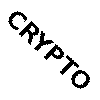
\includegraphics[width=\textwidth,frame]{./Illustrations/KeyReuse/Crypto.png}
    \caption{Second plaintext.}
  \end{subfigure}

  \begin{subfigure}[b]{.4\textwidth}
    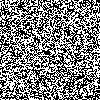
\includegraphics[width=\textwidth]{./Illustrations/KeyReuse/BrokenEncrypted.png}
    \caption{First ciphertext.}
  \end{subfigure}
  \begin{subfigure}[b]{.4\textwidth}
    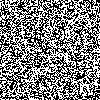
\includegraphics[width=\textwidth]{./Illustrations/KeyReuse/CryptoEncrypted.png}
    \caption{Second ciphertext.}
  \end{subfigure}

  \begin{subfigure}[b]{.4\textwidth}
    
\includegraphics[width=\textwidth]{./Illustrations/KeyReuse/Key.png}
    \caption{Reused key.}
  \end{subfigure}
  \begin{subfigure}[b]{.4\textwidth}
    
\includegraphics[width=\textwidth]{./Illustrations/KeyReuse/CiphertextsXOR.png}
    \caption{XOR of ciphertexts.}
  \end{subfigure}

  \caption{Two plaintexts, the re-used key, their respective
    ciphertexts, and the XOR of the ciphertexts. Information about the
    plaintexts clearly leaks through when we XOR the ciphertexts.}
  \label{fig:multitimepad}
\end{figure}
\subsection{Crib-dragging}
\label{sec-2-1-5-3}

A classical approach to breaking multi-time pad systems involves
\enquote{crib-dragging}, a process that uses small sequences that are expected
to occur with high probability. Those sequences are called \enquote{cribs}.
The name crib-dragging originated from the fact that these small
\enquote{cribs} are dragged from left to right across each ciphertext, and
from top to bottom across the ciphertexts, in the hope of finding a
match somewhere in. Those matches form the sites of the start, or
\enquote{crib}, if you will, of further decryption.

The idea is fairly simple. Suppose we have several encrypted messages
$C_i$ encrypted with the same \enquote{one-time} pad $K$.\footnote{We use capital
letters when referring to an entire message, as opposed to just bits
of a message.} If we could correctly guess the plaintext for one of
the messages, let's say $C_j$, we'd know $K$:

\begin{eqnarray*}
C_j \xor P_j
&=& (P_j \xor K) \xor P_j \\
&=& K \xor P_j \xor P_j \\
&=& K \xor 0 \\
&=& K
\end{eqnarray*}

Since $K$ is the shared secret, we can now use it to decrypt all of
the other messages, just as if we were the recipient:

\[
P_i = C_i \xor K \qquad \text{for all }i
\]

Since we usually can't guess an entire message, this doesn't actually
work. However, we might be able to guess parts of a message.

If we guess a few plaintext bits correctly for \emph{any} of the messages,
that would reveal the key bits at that position for \emph{all} of the
messages, since $k = c_i \xor p_i$. Hence, all of the plaintext bits
at that position are revealed: using that value for $k$, we can
compute the plaintext bits $p_i = c_i \xor k$ for all the other
messages.

Guessing parts of the plaintext is a lot easier than guessing the
entire plaintext. Suppose we know that the plaintext is in English.
There's some sequences that we know will occur very commonly, for
example (the \verb*| | symbol denotes a space):

\begin{itemize}
\item \verb*| the |, variants like \verb*|. The |
\item \verb*| of | and variants
\item \verb*| to | and variants
\item \verb*| and |(less common at the start of a sentence)
\item \verb*| a | and variants
\end{itemize}

If we know more about the plaintext, we can make even better guesses.
For example, if it's HTTP serving HTML, we would expect to see things
like \texttt{Content-Type}, \texttt{<a>}, and so on.

That only tells us which plaintext sequences are likely, giving us
likely guesses. How do we tell if any of those guesses are correct? If
our guess is correct, we know all the other plaintexts at that
position as well, using the technique described earlier. We could
simply look at those plaintexts and decide if they look correct. For
example, if they also contain English text, we'd expect to see a lot
of letters e, t, a, o, i, n. If we're seeing binary nonsense instead,
we know that the guess was probably incorrect, or perhaps that message
is actually binary data.

These small, highly probable sequences are called \enquote{cribs} because
they're the start of a larger decryption process. Suppose your crib,
\verb*| the |, was successful and found the five-letter sequence
\verb*|t thr| in another message. You can then use a dictionary to
find common words starting with \texttt{thr}, such as \texttt{through}. If that
guess were correct, it would reveal four more bytes in all of the
ciphertexts, which can be used to reveal even more. Similarly, you can
use the dictionary to find words ending in \texttt{t}.

This becomes even more effective for some plaintexts that we know more
about. If some HTTP data has the plaintext \texttt{ent-Len} in it, then we
can expand that to \verb*|Content-Length: |, revealing many more
bytes.

While this technique works as soon as two messages are encrypted with
the same key, it's clear that this becomes even easier with more
ciphertexts using the same key, since all of the steps become more
effective:

\begin{itemize}
\item We get more cribbing positions.
\item More plaintext bytes are revealed with each successful crib and
guess, leading to more guessing options elsewhere.
\item More ciphertexts are available for any given position, making guess
validation easier and sometimes more accurate.
\end{itemize}

These are just simple ideas for breaking multi-time pads. While
they're already quite effective, people have invented even more
effective methods by applying advanced, statistical models based on
natural language analysis. This only demonstrates further just how
broken multi-time pads are. \cite{mason:nltwotimepads}
\section{Remaining problems}
\label{sec-2-1-6}

Real one-time pads, implemented properly, have an extremely strong
security guarantee. It would appear, then, that cryptography is over:
encryption is a solved problem, and we can all go home. Obviously,
that's not the case.

One-time pads are impractical: the key is at least as large as all
information you'd like to transmit put together. Plus, you'd have to
exchange those keys securely, ahead of time, with all people you'd
like to communicate with. We'd like to communicate securely with
everyone on the Internet, and that's an impossibly large number of
people. Furthermore, since the keys have to consist of truly random
data for its security property to hold, key generation is fairly
difficult and time-consuming without specialized hardware.

One-time pads pose a trade off. It's an algorithm with a security
guarantee, but it also has extremely impractical key exchange
requirements. However, as we'll see throughout this book, secure
symmetric encryption algorithms aren't the problem. Cryptographers
have designed plenty of those, while practical key management remains
one of the toughest challenges facing modern cryptography. One-time
pads may solve a problem, but it's the wrong problem.

While they may have their uses, they're obviously not a panacea. We
need something with manageable key sizes while maintaining secrecy. We
need ways to negotiate keys over the Internet with people we've never
met before.
\chapter{Block ciphers}
\label{sec-2-2}

\begin{quotation}
Few false ideas have more firmly gripped the minds of so many intelligent men
than the one that, if they just tried, they could invent a cipher that no one
could break.
\sourceatright{David Kahn}
\end{quotation}

\section{Description}
\label{sec-2-2-1}
A \gls{block cipher} is an algorithm that allows us to encrypt blocks
of a fixed length. It provides an encryption function $E$, that takes
a key $k$ and a plaintext block $P$, and produces a ciphertext block
$C$:

\begin{equation}
C = E(k, P)
\end{equation}

The plaintext and ciphertext blocks are sequences of bytes. They are
always the same size as one another, and that size is fixed by the
block cipher: it's called the block cipher's \emph{block size}.

Once we've encrypted plaintext blocks into ciphertext blocks, they
later have to be decrypted again to recover the original plaintext
block. This is done using a decryption function $D$, which takes the
ciphertext block $C$ and the key $k$ (the same one used to encrypt the
block) as inputs, and produces the original plaintext block $P$.

\begin{equation}
P = D(k, C)
\end{equation}

Or, in blocks:

\includegraphics[width=.9\linewidth]{./Illustrations/BlockCipher/BlockCipher.pdf}

\newcommand{\permutationimg}[1] {
\begin{figure}[ht!]
  \centering
  \includegraphics[width=.3\linewidth]{./Illustrations/BlockCipher/Set#1.pdf}

  \includegraphics[width=.2\linewidth]{./Illustrations/BlockCipher/Arrow#1.pdf}
\end{figure}
}

A block cipher is a \emph{keyed permutation}. It's a \emph{permutation}, because
the block cipher maps every possible block to some other block. It's
also a \emph{keyed} permutation, because the key determines exactly which
blocks map to which.

We'll illustrate this by looking at a block cipher with a
impractically tiny 3-bit block size, so $2^3 = 8$ possible blocks.
Encryption would look like this:

\permutationimg{Ek}

The points $a, b, c\ldots$ are blocks. The arrows show which blocks
map to which blocks: that the block at the start of the arrow,
encrypted using $E$ under key $k$, is mapped to the block at the end
of the arrow. For example, $E(k, a) = b$.

When you're decrypting instead of encrypting, the block cipher just
computes the inverse permutation. We get the same illustrations, with
all the arrows going in the other direction:

\permutationimg{Dk}

The only way to know which block maps to which other block, is to know
the key. A different key will lead to a completely different set of
arrows, for example under $k^{\prime}$:

\permutationimg{Ekprime}

Knowing a bunch of (input, output) pairs shouldn't give you any
information about any other (input, output) pairs\footnote{The attentive
reader may have noticed that this breaks in the extremes: if you know
all but one of the pairs, then you know the last one by exclusion.}.
As long as we're talking about a hypothetical perfect block cipher,
there's no easier way to decrypt a block other than to \enquote{brute-force}
the key: i.e. just try every single one of them until you find the
right one.

Our toy illustration block cipher only has 3 bit blocks, or $2^3 = 8$
possibilities. Real, modern block ciphers have much larger block
sizes, such as 128 bits, or $2^{128}$ possible blocks. Mathematics
tells us that there are $n!$ (pronounced \emph{n factorial}) different
permutations of an $n$ element set. It's defined as the product of all
of the numbers from 1 up to and including $n$:

\[
n! = 1 \cdot 2 \cdot 3 \cdot \ldots \cdot (n - 1) \cdot n
\]

Factorials grow incredibly quickly. For example, $5! = 120$, $10! =
3628800$, and the rate continues to increase. The number of
permutations of the set of blocks of a cipher with a 128 bit block
size is $(2^{128})!$. Just $2^{128}$ is large already (it takes 38
digits to write it down), so $(2^{128})!$ is a mind-bogglingly huge
number, impossible to comprehend. Common key sizes are only in the
range of 128 to 256 bits, yielding $2^{128}$ to $2^{256}$
possibilities. That means that only a tiny fraction of all possible
permutations are possible. That's okay: that tiny fraction is still
more than large enough that it's impossible for an attacker to just
try them all.

Of course, a block cipher should be as easy to compute as possible,
as long as it doesn't sacrifice any of the above properties.
\section{\label{AES}AES}
\label{sec-2-2-2}

The most common block cipher in current use is \gls{AES}, the Advanced
Encryption Standard. Prior to being chosen as the Advanced Encryption
Standard, the algorithm was known as Rijndael. Rijndael defined a
family of block ciphers, with block sizes and key sizes that could be
any multiple of 32 bits between 128 bits and 256 bits.
\cite{daemen:aes} When Rijndael became \hyperref[AES]{AES} through the \gls{FIPS}
standardization process, the parameters were restricted to a block
size of 128 bits and keys sizes of 128, 192 and 256 bits.
\cite{fips:aes}

REVIEW: Show how \hyperref[AES]{AES} works internally?

There are no practical attacks known against \hyperref[AES]{AES}. While there have
been some developments in the last few years, most of them involve
related-key attacks \cite{cryptoeprint:2009:317}, some of them only on
reduced-round versions of \hyperref[AES]{AES} \cite{cryptoeprint:2009:374}.

A related key attack involves making some predictions about how \hyperref[AES]{AES}
will behave with two different keys with some specific mathematical
relation. Those predictions provide some information about what
identical (input, output) pairs will look like under those different
keys. Most of these attacks attempt to recover the key entirely,
completely breaking the encryption. While an ideal block cipher
wouldn't be vulnerable to a related key attack, no system in the real
world should ever end up with such related keys. If it does, things
have gone so completely wrong that all further bets are off.
\section{DES and 3DES}
\label{sec-2-2-3}

The \gls{DES} is one of the oldest block ciphers that saw widespread
use. It was published as an official \gls{FIPS} standard in 1977. It
is no longer considered secure, mainly due to its tiny key size of 56
bits. (The DES algorithm actually takes a 64 bit key input, but the
remaining 8 bits are only used for parity checking, and are discarded
immediately.) It shouldn't be used in new systems. On modern hardware,
DES can be brute forced in less
 than a day. \cite{sciengines:breakdes}

In an effort to extend the life of the DES algorithm, in a way that
allowed much of the spent hardware development effort to be reused,
people came up with 3DES: a scheme where input is first encrypted,
then decrypted, then encrypted again:

\begin{equation}
C = E_{DES}(k_1, D_{DES}(k_2, E_{DES}(k_3, p)))
\end{equation}

This scheme provides two improvements:

\begin{itemize}
\item By applying the algorithm three times, the cipher becomes harder to
attack directly through cryptanalysis.
\item By having the option of using many more total key bits, spread over
the three keys, the set of all possible keys becomes much larger,
making brute-forcing impractical.\footnote{The set of all keys is
   commonly called the keyspace.}
\end{itemize}

The three keys could all be chosen independently (yielding 168 key
bits), or $k_3 = k_1$ (yielding 112 key bits), or $k_1 = k_2 = k_3$,
which, of course, is just plain old DES (with 56 key bits). In the
last keying option, the middle decryption reverses the first
encryption, so you really only get the effect of the last encryption.
This is intended as a backwards compatibility mode for existing DES
systems. If 3DES had been defined as $E(k_1, E(k_2, E(k_3, p)))$, it
would've been impossible to use 3DES implementations for systems that
required compatibility with DES.

Some attacks on 3DES are known, reducing their effective security.
While breaking 3DES with the first keying option is currently
impractical, 3DES is a poor choice for any modern cryptosystem. The
security margin is already small, and continues to shrink as
cryptographic attacks improve and processing power grows.

Far better alternatives, such as \hyperref[AES]{AES}, are available. Not only are they
more secure than 3DES, they are also generally much, much faster. On
the same hardware and in the same \gls{mode of operation} (we'll
explain what that means in the next chapter), \hyperref[AES]{AES}-128 only takes 12.6
cycles per byte, while 3DES takes up to 134.5 cycles per byte.
\cite{cryptopp:bench} Despite being worse from a security point of
view, it is literally an order of magnitude slower.

While more iterations of DES might increase the security margin, they
aren't used in practice. First of all, the process has never been
standardized beyond three iterations. Also, the performance only
becomes worse as you add more iterations. Finally, increasing the key
bits has diminishing security returns, only increasing the security
level of the resulting algorithm by a smaller amount as the number of
key bits increases. While 3DES with keying option 1 has a key length
of 168 bits, the effective security level is estimated at only 112
bits.

Even though 3DES is significantly worse in terms of performance and
slightly worse in terms of security, 3DES is still the workhorse of
the financial industry. With a plethora of standards already in
existence and new ones continuing to be created, in such an extremely
technologically conservative industry where Fortran and Cobol still
reign supreme on massive mainframes, it will probably continue to be
used for many years to come, unless there are some large cryptanalytic
breakthroughs that threaten the security of 3DES.

TODO: Explain security levels? See also: explain entropy?
\section{Remaining problems}
\label{sec-2-2-4}
Even with block ciphers, there are still some unsolved problems.

For example, we can only send messages of a very limited length: the
block length of the block cipher. Obviously, we'd like to be able to
send much larger messages, or, ideally, streams of indeterminate size.
We'll address this problem with a \hyperref[sec-2-3]{stream cipher}.

Although we have reduced the key size drastically (from the total size
all data ever sent under a one-time pad scheme versus a few bytes for
most block ciphers), we still need to address the issue of agreeing on
those few key bytes, potentially over an insecure channel. We'll
address this problem in a later chapter with a \hyperref[sec-2-4]{key exchange protocol}.
\chapter{Stream ciphers}
\label{sec-2-3}
\section{Description}
\label{sec-2-3-1}
A stream cipher is a symmetric encryption algorithm that encrypts a
stream of bits. Ideally, that stream could be as long as we'd like;
real-world stream ciphers have limits, but they are normally
sufficiently large that they don't pose a practical problem.
\section{A naive attempt with block ciphers\label{ECB-mode}}
\label{sec-2-3-2}

Let's try to build a stream cipher using the tools we already have.
Since we already have block ciphers, we could simply divide an
incoming stream into different blocks, and encrypt each block:

\begin{equation}
\begin{matrix}
\underbrace{\mathtt{abcdefgh}} & \underbrace{\mathtt{ijklmno}} & \underbrace{\mathtt{pqrstuvw}} & ...\\
\downarrow & \downarrow & \downarrow & \\
\overbrace{\mathtt{APOHGMMW}} & \overbrace{\mathtt{PVMEHQOM}} & \overbrace{\mathtt{MEEZSNFM}} & ...
\end{matrix}
\end{equation}

This scheme is called \gls{ECB mode}, and it is one of the many ways
that block ciphers can be used to construct stream ciphers.
Unfortunately, while being very common in home-grown cryptosystems, it
poses very serious security flaws. For example, in ECB mode, identical
input blocks will always map to identical output blocks:

\begin{equation}
\begin{matrix}
\underbrace{\mathtt{abcdefgh}} & \underbrace{\mathtt{abcdefgh}} & \underbrace{\mathtt{abcdefgh}} & ...\\
\downarrow & \downarrow & \downarrow & \\
\overbrace{\mathtt{APOHGMMW}} & \overbrace{\mathtt{APOHGMMW}} & \overbrace{\mathtt{APOHGMMW}} & ...
\end{matrix}
\end{equation}

At first, this might not seem like a particularly serious problem.
Assuming the block cipher is secure, it doesn't look like an attacker
would be able to decrypt anything. By dividing the ciphertext stream
up into blocks, an attacker would only be able to see that a
ciphertext block, and therefore a plaintext block, was repeated.

We'll now illustrate the many flaws of ECB mode with two attacks.
First, we'll exploit the fact that repeating plaintext blocks result
in repeating ciphertext blocks, by visually inspecting an encrypted
image. Then, we'll demonstrate that attackers can often decrypt
messages encrypted in ECB mode by communicating with the person
performing the encryption.

\subsection{Visual inspection of an encrypted stream}
\label{sec-2-3-2-1}

To demonstrate that this is, in fact, a serious problem, we'll use a
simulated block cipher of various block sizes and apply it to an
image\footnote{This particular demonstration only works on uncompressed
bitmaps. For other media, the effect isn't significantly less damning:
it's just less visual.}. We'll then visually inspect the different
outputs.

\begin{figure}[p]
  \centering

  \begin{subfigure}[b]{.45\textwidth}
    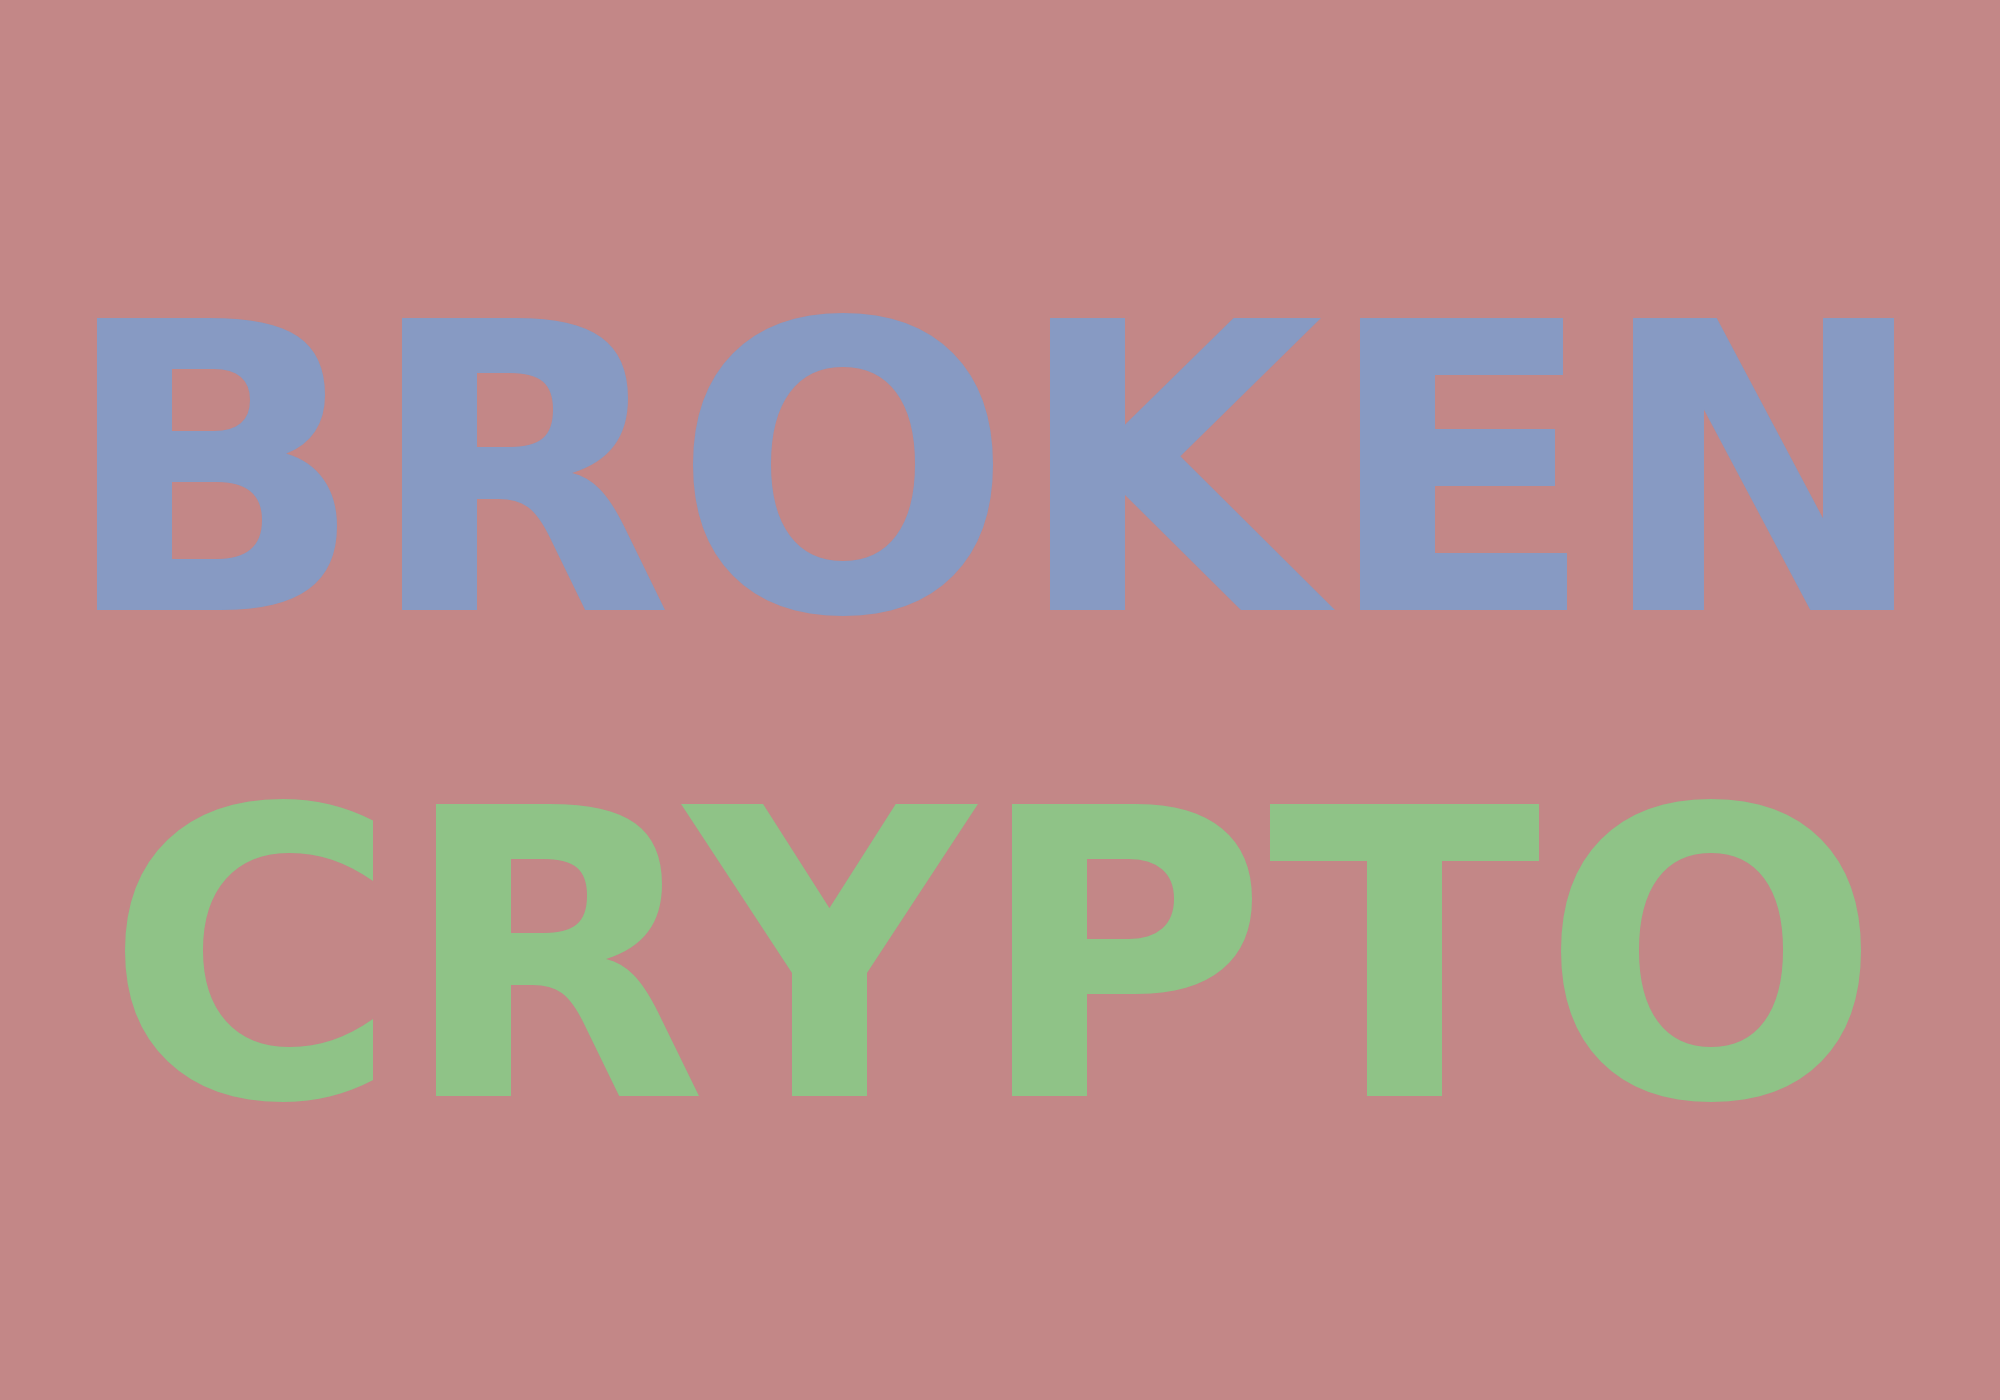
\includegraphics[width=\textwidth]{./Illustrations/ECB/Plaintext.png}
    \caption{Plaintext image, 2000 by 1400 pixels, 24 bit color depth.}
    \label{fig:ECBDemoPlaintext}
  \end{subfigure}
  \quad
  \begin{subfigure}[b]{.45\textwidth}
    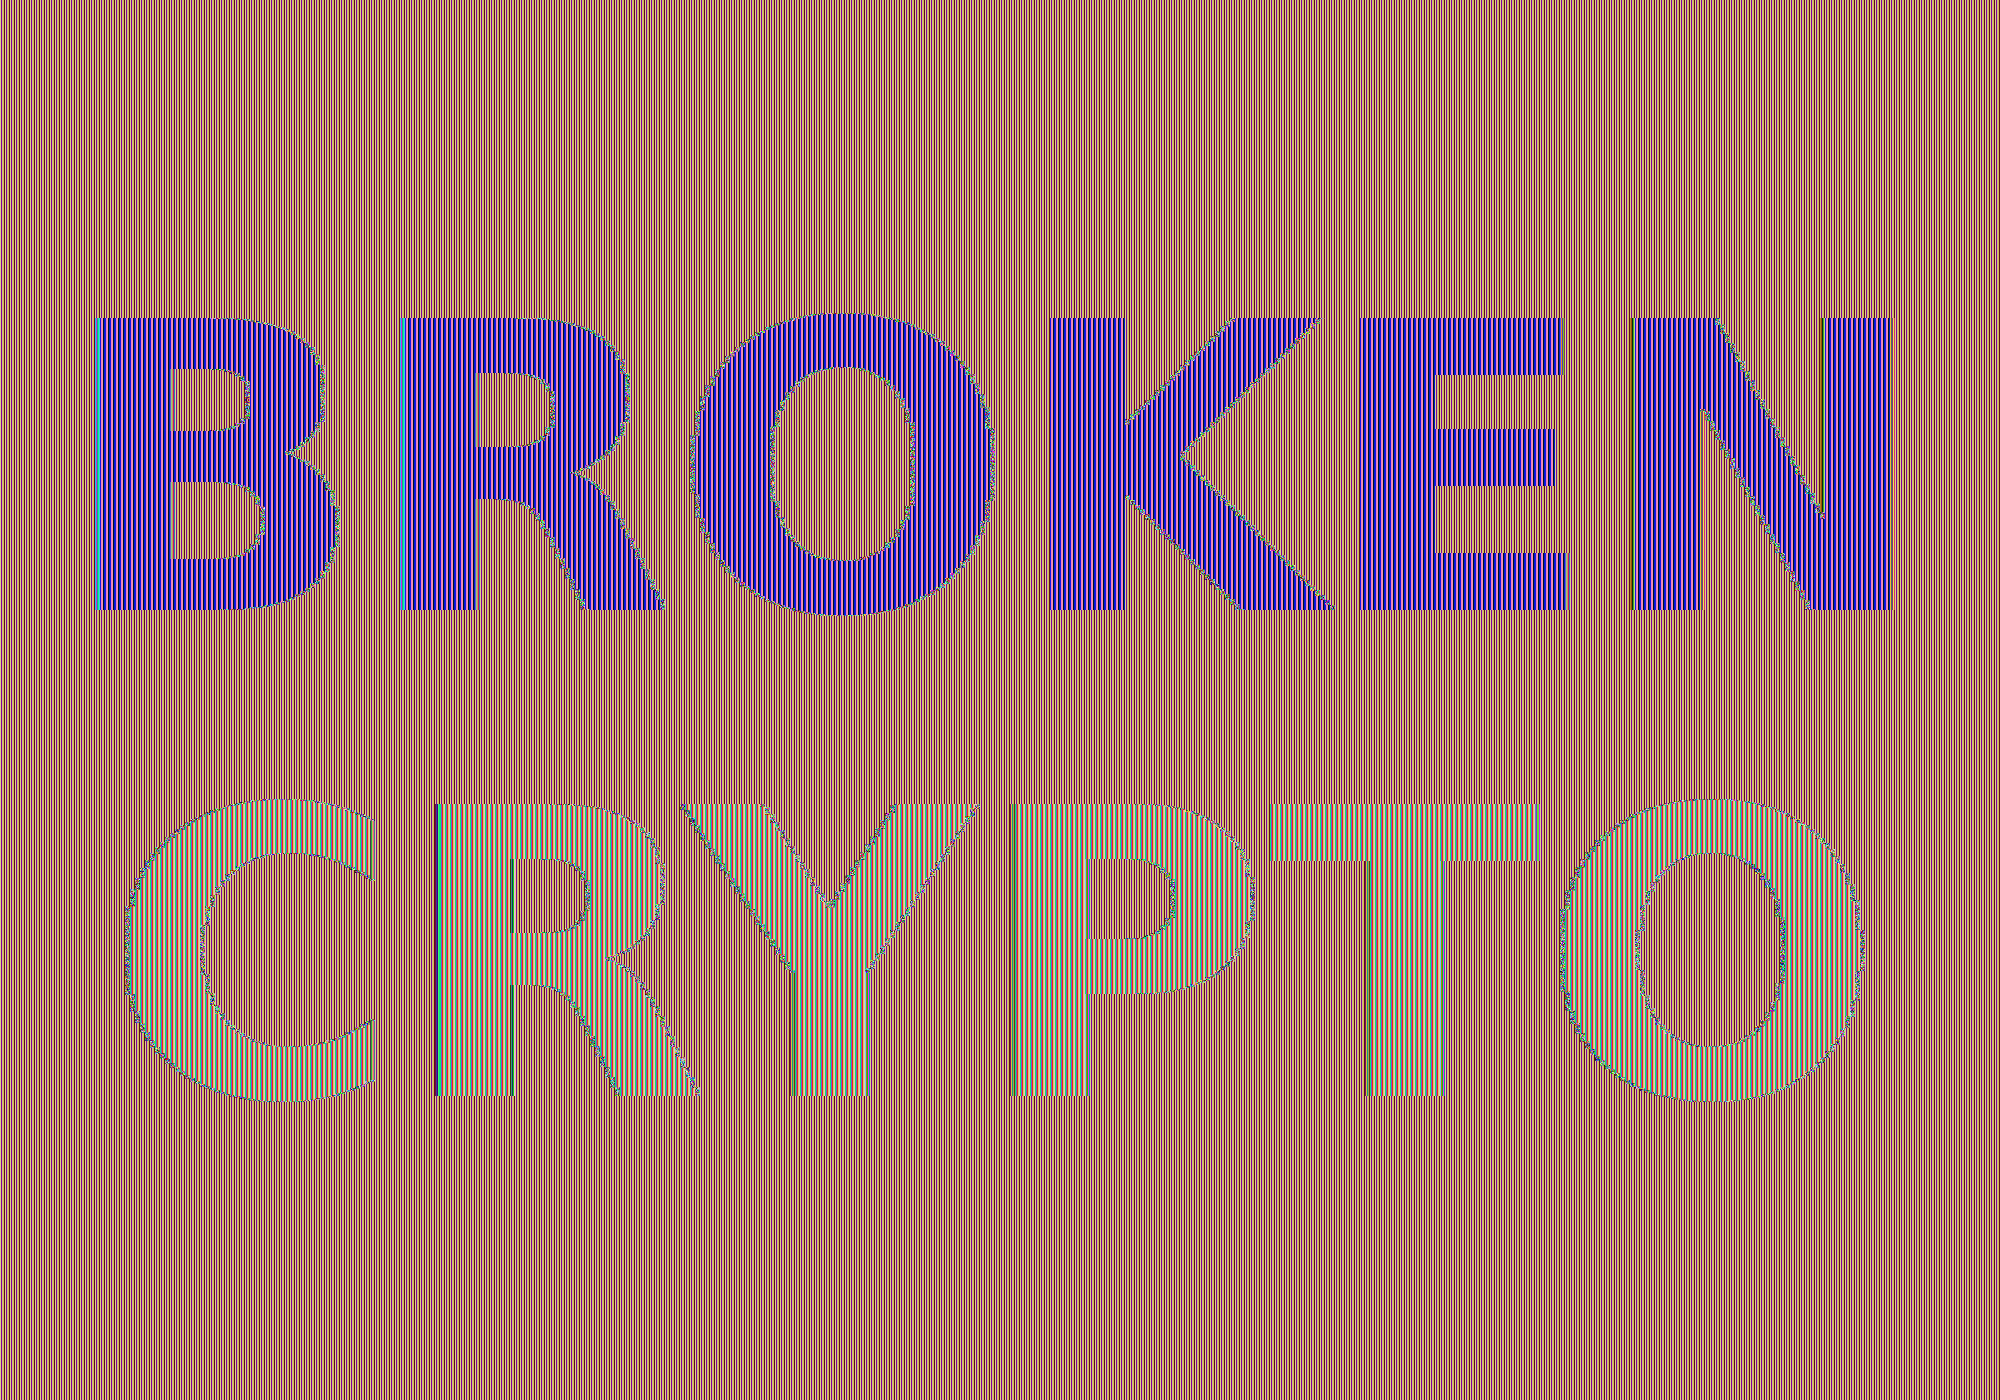
\includegraphics[width=\textwidth]{./Illustrations/ECB/Ciphertext5.png}
    \caption{ECB mode ciphertext, 5 pixel (120 bit) block size.}
    \label{fig:ECBDemo5px}
  \end{subfigure}

  \begin{subfigure}[b]{.45\textwidth}
    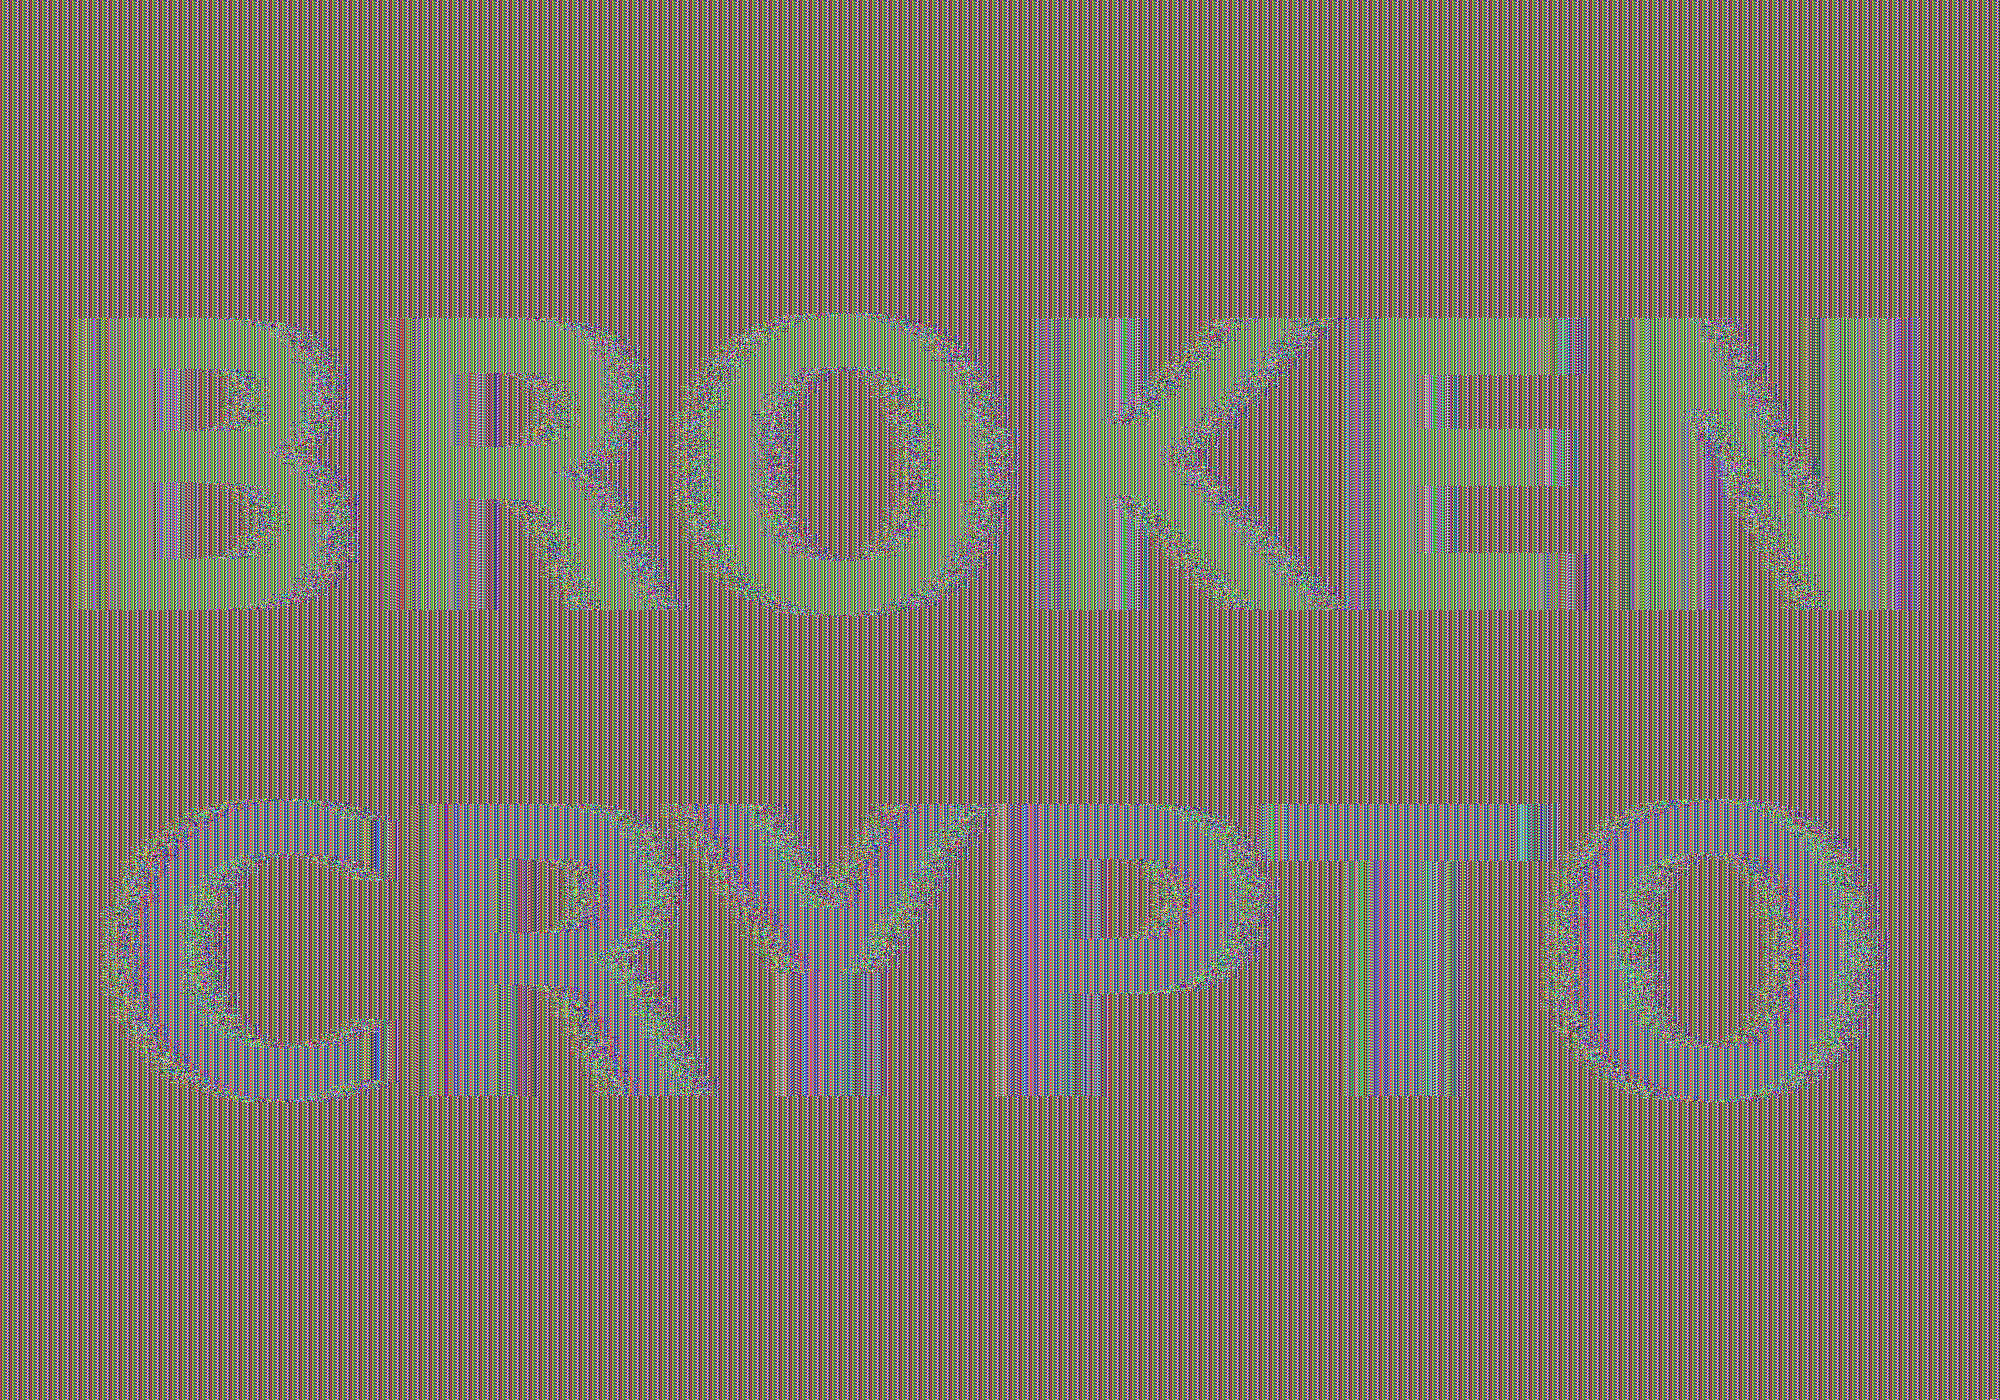
\includegraphics[width=\textwidth]{./Illustrations/ECB/Ciphertext30.png}
    \caption{ECB mode ciphertext, 30 pixel (720 bit) block size.}
  \end{subfigure}
  \quad
  \begin{subfigure}[b]{.45\textwidth}
    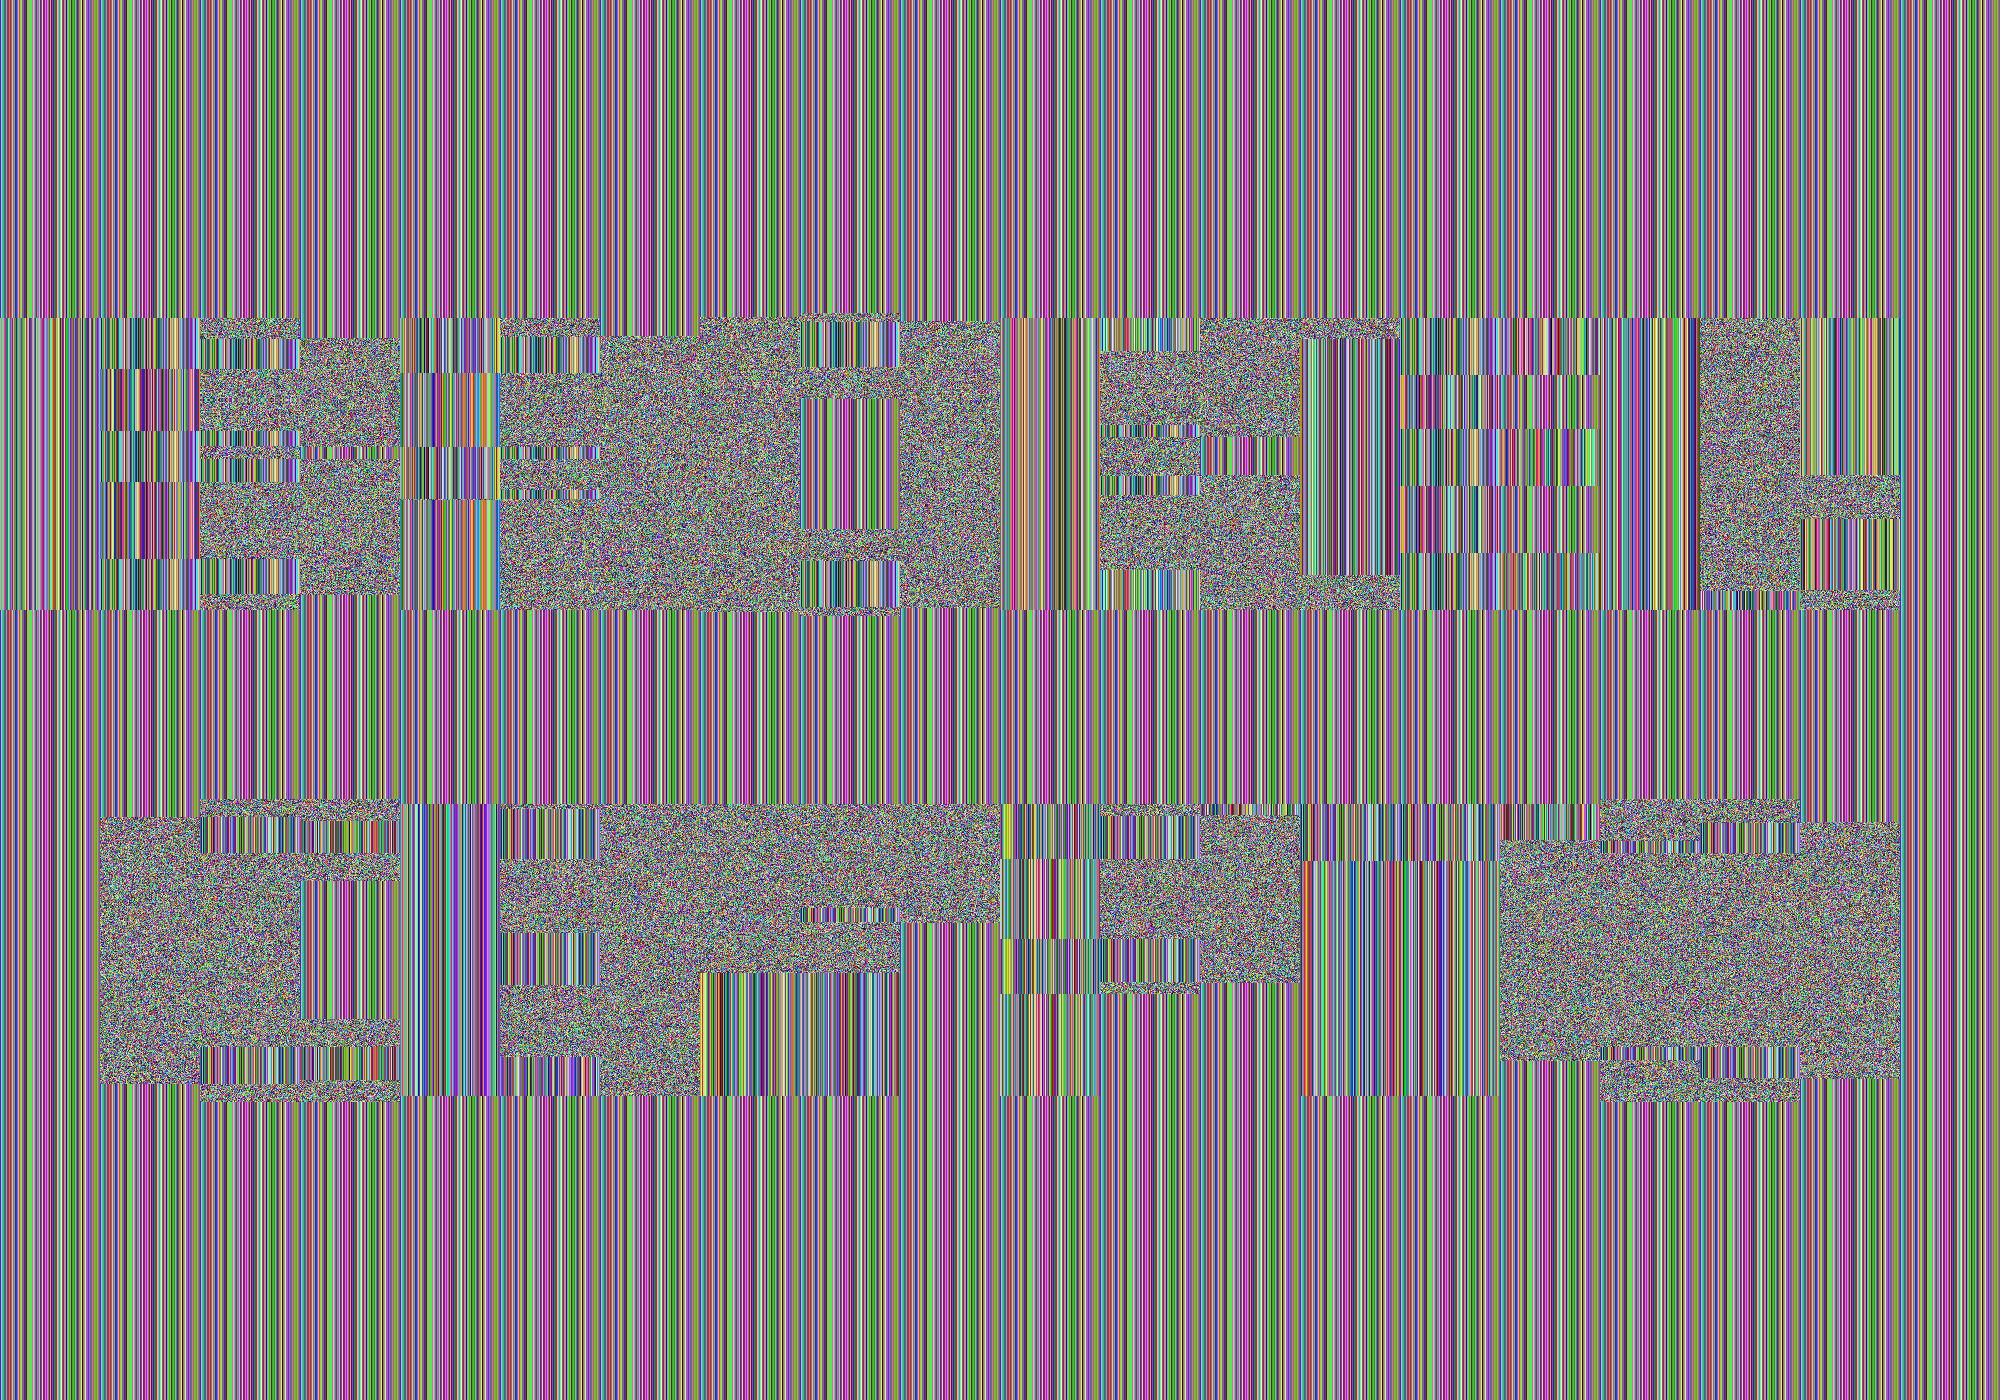
\includegraphics[width=\textwidth]{./Illustrations/ECB/Ciphertext100.png}
    \caption{ECB mode ciphertext, 100 pixel (2400 bit) block size.}
  \end{subfigure}

  \begin{subfigure}[b]{.45\textwidth}
    
\includegraphics[width=\textwidth]{./Illustrations/ECB/Ciphertext400.png}
    \caption{ECB mode ciphertext, 400 pixel (9600 bit) block size.}
  \end{subfigure}
  \quad
  \begin{subfigure}[b]{.45\textwidth}
    \includegraphics[width=\textwidth]{./Illustrations/ECB/Random.png}
    \caption{Ciphertext under idealized encryption.}
    \label{fig:ECBDemoIdealizedCiphertext}
  \end{subfigure}

  \caption{Plaintext image with ciphertext images under idealized
    encryption and ECB mode encryption with various block sizes.
    Information about the macro-structure of the image clearly leaks.
    This becomes less apparent as block sizes increase, but only at
    block sizes far larger than typical block ciphers. Only the first
    block size (figure \subref{fig:ECBDemo5px}, a block size of 5
    pixels or 120 bits) is realistic.}
\end{figure}

Because identical blocks of pixels in the plaintext will map to
identical blocks of pixels in the ciphertext, the global structure of
the image is largely preserved.

As you can see, the situation appears to get slightly better with
larger block sizes, but the fundamental problem still remains: the
macrostructure of the image remains visible in all but the most
extreme block sizes. Furthermore, all but the smallest of these block
sizes are unrealistically large. For an uncompressed bitmap with three
color channels of 8 bit depth, each pixel takes 24 bits to store.
Since the block size of \hyperref[AES]{AES} is only 128 bits, that would equate to
$5.\overline{3}$ pixels \footnote{The line over the $3$ in $5.\overline{3}$
means it repeats, so the value is $5.333\ldots$.} per block,
significantly less than the larger block sizes in the example. But \hyperref[AES]{AES}
is the workhorse of modern block ciphers---it can't be at fault,
certainly not because of an insufficient block size.

When we look at a picture of what would happen with an idealized
encryption scheme, we notice that it looks like random noise. Keep in
mind that \enquote{looking like random noise} doesn't mean something is
properly encrypted: it just means that we can't inspect it using
methods this trivial.
\subsection{Encryption oracle attack}
\label{sec-2-3-2-2}

In the previous section, we've focused on how an attacker can inspect
a ciphertext encrypted using \gls{ECB mode}. That's a \emph{passive},
ciphertext-only attack. It's passive because the attacker doesn't
really interfere in any communication; they're simply examining a
ciphertext. In this section, we'll study an \emph{active} attack, where the
attacker actively communicates with their target. We'll see how the
active attack can enable an attacker to decrypt ciphertexts encrypted
using ECB mode.

To do this, we'll introduce a new concept called an \gls{oracle}.
Formally defined oracles are used in the study of computer science,
but for our purposes it's sufficient to just say that an oracle is
something that will compute some particular function for you.

In our case, the oracle will perform a specific encryption for the
attacker, which is why it's called an \gls{encryption oracle}. Given
some data $A$ chosen by the attacker, the oracle will encrypt that
data, followed by a secret suffix $S$, in ECB mode. Or, in symbols:

\[
C = ECB(E_k, A \| S)
\]

You can see why the concept of an oracle is important here: the
attacker would not be able to compute $C$ themselves, since they do
not have access to the encryption key $k$ or the secret suffix $S$.
The goal of the oracle is for those values to remain secret, but we'll
see how an attacker can recover $S$ by inspecting the ciphertext $C$
for many carefully chosen values of the prefix $A$.
\subsection{Decrypting a block using the oracle}
\label{sec-2-3-2-3}

The attacker starts by sending in a plaintext $A$ that's just one byte
shorter than the block size. That means the block that's being
encrypted will consist of those bytes, plus the first byte of $S$,
which we'll call $s_0$. The attacker remembers the encrypted block.
They don't know the value of $s_0$ yet, but now they do know the value
of the first encrypted block: $E_k(A \| s_0)$. In the illustration,
this is block $C_{R1}$:

\newcommand{\ecbencoracleimg}[1]{
\begin{figure}[ht!]
\centering
\includegraphics[width=.60\linewidth]{./Illustrations/ECBEncryptionOracle/#1.pdf}
\end{figure}
}

\ecbencoracleimg{RememberFirst}

Then, the attacker tries a full-size block, trying all possible values
for the final byte. Eventually, they'll find the value of $s_0$; they
know the guess is correct because the resulting ciphertext block will
match the ciphertext block $C_{R1}$ they remembered earlier.

\ecbencoracleimg{GuessFirst}

The attacker can repeat this for the penultimate byte. They submit a
plaintext $A$ that's two bytes shorter than the block size. The oracle
will encrypt a first block consisting of that $A$ followed by the
first two bytes of the secret suffix, $s_0s_1$. The attacker remembers
that block.

\ecbencoracleimg{RememberSecond}

Since the attacker already knows $s_0$, they try $A \|
s_0$ followed by all possible values of $s_1$. Eventually they'll
guess correctly, which, again, they'll know because the ciphertext
blocks match:

\ecbencoracleimg{GuessSecond}

The attacker can rinse and repeat, eventually decrypting an entire
block. This allows them to brute-force a block in $p \cdot b$
attempts, where $p$ is the number of possible values for each byte
(so, for 8-bit bytes, that's $2^8 = 256$) and $b$ is the block size.
Normally, they'd have to try all of the possible combinations, which
would be:

\[
\underbrace{p \cdot p \ldots \cdot p}_{b \ \mathrm{positions}} = p^b
\]

For a typical block size of 16 bytes (or 128 bits), brute forcing
would mean trying $256^{16}$ combinations. That's a huge, 39-digit
number. It's so large that trying all of those combinations is
considered impossible. This attack allows an attacker to do it in at
most $256 \cdot 16 = 4096$ tries, a far more manageable number.
\subsection{Conclusion}
\label{sec-2-3-2-4}

In the real world, block ciphers are used in systems that encrypt
large amounts of data all the time. We've seen that when using
\gls{ECB mode}, an attacker can both analyze ciphertexts to recognize
repeating patterns, and even decrypt messages when given access to an
\gls{encryption oracle}.

Even when we use idealized block ciphers with unrealistic properties,
such as block sizes of more than a thousand bits, an attacker ends up
being able to decrypt the ciphertexts. Real world block ciphers only
have more limitations than our idealized examples, such as much
smaller block sizes.

We aren't even taking into account any potential weaknesses in the
block cipher. It's not \hyperref[AES]{AES} (or our test block ciphers) that cause this
problem, it's our ECB construction. Clearly, we need something better.
\section{Block cipher modes of operation}
\label{sec-2-3-3}

One of the more common ways of producing a \gls{stream cipher} is to
use a block cipher in a particular configuration. The compound system
behaves like a stream cipher. These configurations are commonly called
\glspl{mode of operation}. They aren't specific to a particular block
cipher.

\Gls{ECB mode}, which we've just seen, is the simplest such mode of
operation. The letters \verb~ECB~ stand for electronic code book\footnote{Traditionally, modes of operation seem to be referred to by a
three-letter acronym.}. For reasons we've already gone into, ECB mode
is very ineffective. Fortunately, there are plenty of other choices.
\section{\label{CBC-mode}CBC mode}
\label{sec-2-3-4}

\gls{CBC mode}, which stands for cipher block chaining, is a very
common \gls{mode of operation} where plaintext blocks are XORed with
the previous ciphertext block before being encrypted by the block
cipher.

Of course, this leaves us with a problem for the first plaintext
block: there is no previous ciphertext block to XOR it with. Instead,
we pick an \gls{IV}: a random number that takes the place of the
\enquote{first} ciphertext in this construction. \Glspl{initialization vector}
also appear in many other algorithms. An initialization vector should
be unpredictable; ideally, they will be cryptographically random. They
do not have to be secret: IVs are typically just added to ciphertext
messages in plaintext.

The following diagram demonstrates encryption in \hyperref[CBC mode]{CBC-mode}:

\includegraphics[width=.9\linewidth]{./Illustrations/CBC/Encryption.pdf}

Decryption is the inverse construction, with block ciphers in
decryption mode instead of encryption mode:

\includegraphics[width=.9\linewidth]{./Illustrations/CBC/Decryption.pdf}

While \hyperref[CBC mode]{CBC-mode} itself is not inherently insecure (unlike ECB mode),
its particular use in TLS 1.0 was. This eventually led to the
\gls{BEAST} attack, which we'll cover in more detail in the section on
SSL/TLS. The short version is that instead of using unpredictable
\glspl{initialization vector}, for example by choosing random ones,
the previous ciphertext block was used. Unfortunately, it turns out
that attackers figured out how to exploit that property.
\section{\label{CBC-bit-flipping-attacks}CBC bit flipping attacks}
\label{sec-2-3-5}

An interesting attack on \gls{CBC mode} is called a bit flipping
attack. Using a CBC bit flipping attack, attackers can modify
ciphertexts encrypted in \hyperref[CBC mode]{CBC-mode} so that it will have a predictable
effect on the plaintext.

Suppose we have a CBC encrypted ciphertext. This could be, for
example, a cookie. We take a particular ciphertext block, and we flip
some bits in it. What happens to the plaintext?

When we \enquote{flip some bits}, we do that by XORing with a sequence of
bits, which we'll call $X$. If the corresponding bit in $X$ is 1, the
bit will be flipped; otherwise, the bit will remain the same.

\begin{figure}[h!]
\centering
\includegraphics[width=.6\linewidth]{./Illustrations/CBC/BitFlipping.pdf}
\end{figure}

When we try to decrypt the ciphertext block with the flipped bits, we
will get indecipherable\footnote{Excuse the pun.} nonsense. Remember how
CBC decryption works: the output of the block cipher is XORed with the
previous ciphertext block to produce the plaintext block. Now that the
input ciphertext block $C_i$ has been modified, the output of the
block cipher will be some random unrelated block, and, statistically
speaking, nonsense. After being XORed with that previous ciphertext
block, it will still be nonsense. As a result, the produced plaintext
block is still just nonsense. In the illustration, this unintelligible
plaintext block is $P_i^{\prime}$.

However, in the block \emph{after} that, the bits we flipped in the
ciphertext will be flipped in the plaintext as well! This is because,
in CBC decryption, ciphertext blocks are decrypted by the block
cipher, and the result is XORed with the previous ciphertext block.
But since we modified the previous ciphertext block by XORing it with
$X$, the plaintext block $P_{i + 1}$ will also be XORed with $X$. As a
result, the attacker completely controls that ciphertext block, since
they can just flip the bits that aren't the value they want them to
be.

TODO: add previous illustration, but mark the path X takes to
influence P prime \{i + 1\} in red or something

This may not sound like a huge deal at first. If you don't know the
plaintext bytes of that next block, you have no idea which bits to
flip in order to get the plaintext you want.

To illustrate how attackers can turn this into a practical attack,
let's consider a website using cookies. When you register, your chosen
user name is put into a cookie. The website encrypts the cookie and
sends it to your browser. The next time your browser visits the
website, it will provide the encrypted cookie; the website decrypts it
and knows who you are.

An attacker can often control at least part of the plaintext being
encrypted. In this example, the user name is part of the plaintext of
the cookie. Of course, the website just lets you provide whatever
value for the user name you want at registration, so the attacker can
just add a very long string of \verb~Z~ bytes to their user name. The
server will happily encrypt such a cookie, giving the attacker an
encrypted ciphertext that matches a plaintext with many such \verb~Z~ bytes in
them. The plaintext getting modified will then probably be part of
that sequence of \verb~Z~ bytes.

An attacker may have some target bytes that he'd like to see in the
decrypted plaintext, for example, \verb*|;admin=1;|. In order to
figure out which bytes they should flip (so, the value of $X$ in the
illustration), they just XOR the filler bytes (\verb~ZZZ~ \ldots) with that
target. Because two XOR operations with the same value cancel each
other out, the two filler values (\verb~ZZZ~ \ldots) will cancel out, and
the attacker can expect to see \verb|;admin=1;| pop up in the next
ciphertext block:

\begin{eqnarray*}
P^{\prime}_{i + 1} & = & P_{i + 1} \xor X \\
& = & P_{i + 1}
  \xor \mathtt{ZZZZZZZZZ}
  \xor \mathtt{;admin=1;} \\
& = & \mathtt{ZZZZZZZZZ}
  \xor \mathtt{ZZZZZZZZZ}
  \xor \mathtt{;admin=1;} \\
& = &  \mathtt{;admin=1;} \\
\end{eqnarray*}

This attack is another demonstration of an important cryptographic
principle: encryption is not authentication! It's virtually never
sufficient to simply encrypt a message. It \emph{may} prevent an attacker
from reading it, but that's often not even necessary for the attacker
to be able to modify it to say whatever they want it to.
\section{Padding}
\label{sec-2-3-6}

So far, we've conveniently assumed that all messages just happened to
fit exactly in our system of block ciphers, be it CBC or ECB. That
means that all messages happen to be a multiple of the block size,
which, in a typical block cipher such as \hyperref[AES]{AES}, is 16 bytes. Of course,
real messages can be of arbitrary length. We need some scheme to make
them fit. That process is called padding.

\subsection{Padding with zeroes (or some other pad byte)}
\label{sec-2-3-6-1}

One way to pad would be to simply append a particular byte value until
the plaintext is of the appropriate length. To undo the padding, you
just remove those bytes. This scheme has an obvious flaw: you can't
send messages that end in that particular byte value, or you will be
unable to distinguish between padding and the actual message.
\subsection{\label{PKCS-5/PKCS-7-padding}PKCS\#5/PKCS\#7 padding}
\label{sec-2-3-6-2}

A better, and much more popular scheme, is \hyperref[PKCS\#5/PKCS\#7 padding]{PKCS-5/PKCS-7-padding}.

PKCS\#5, PKCS\#7 and later CMS padding are all more or less the same
idea\footnote{Technically, PKCS\#5 padding is only defined for 8 byte block
sizes, but the idea clearly generalizes easily, and it's also the most
commonly used term.}. Take the number of bytes you have to pad, and
pad them with that many times the byte with that value. For example,
if the block size is 8 bytes, and the last block has the three bytes
\texttt{12 34 45}, the block becomes \texttt{12 34 45 05 05 05 05 05} after padding.

If the plaintext happened to be exactly a multiple of the block size,
an entire block of padding is used. Otherwise, the recipient would
look at the last byte of the plaintext, treat it as a padding length,
and almost certainly conclude the message was improperly padded.

This scheme is described in \cite{cms:padding}.
\section{CBC padding attacks}
\label{sec-2-3-7}

We can refine \hyperref[CBC bit flipping attacks]{CBC-bit-flipping-attacks} to trick a recipient into
decrypting arbitrary messages!

As we've just discussed, \gls{CBC mode} requires padding the message
to a multiple of the block size. If the padding is incorrect, the
recipient typically rejects the message, saying that the padding was
invalid. We can use that tiny bit of information about the padding of
the plaintext to iteratively decrypt the entire message.

The attacker will do this, one ciphertext block at a time, by trying
to get an entire plaintext block worth of valid padding. We'll see
that this tells them the decryption of their target ciphertext block,
under the block cipher. We'll also see that you can do this
efficiently and iteratively, just from that little leak of information
about the padding being valid or not.

It may be helpful to keep in mind that a CBC padding attack does not
actually attack the padding for a given message; instead the attacker
will be \emph{constructing} paddings to decrypt a message.

To mount this attack, an attacker only needs two things:

\begin{enumerate}
\item A target ciphertext to decrypt
\item A \emph{padding oracle}: a function that takes ciphertexts and tells
the attacker if the padding was correct
\end{enumerate}

In this chapter, we'll assume that \hyperref[PKCS\#5/PKCS\#7 padding]{PKCS-5/PKCS-7-padding} is being
used, since that's the most popular option. The attack is general
enough to work on other kinds of padding, with minor modifications.

\subsection{Decrypting the first byte}
\label{sec-2-3-7-1}

The attacker fills a block with arbitrary bytes $R = r_1, r_2\ldots
r_b$. They also pick a target block $C_i$ from the ciphertext that
they'd like to decrypt. The attacker asks the padding oracle if $R \|
C_i$ has valid padding. Statistically speaking, such a random
plaintext block probably won't have valid padding: the odds are in the
half-a-percent ballpark. If by pure chance the message happens to
already have valid padding, they can simply skip the next step.

\begin{figure}[ht!]
\centering
\includegraphics[width=.8\linewidth]{./Illustrations/CBC/PaddingAttack.pdf}
\end{figure}

Next, the attacker tries to modify the message so that it does have
valid padding. They can do that by playing with the last byte of the
plaintext: eventually that byte will be \verb~01~, which is always valid
padding. In order to modify the last byte of a plaintext block, the
attacker modifies the last byte of the \emph{previous} ciphertext block.
This works exactly like it did with \hyperref[CBC bit flipping attacks]{CBC-bit-flipping-attacks}. That
previous ciphertext block is the block $R$, so the byte being modified
is the last byte of $R$, $r_b$.

One way to try all values for that last byte of $R$ is to XOR it with
all values up to 256, since a byte has 256 possible values.
Eventually, the padding oracle will report that for some ciphertext
block $R$, the decrypted plaintext of $R \| C_i$ has valid padding.
\subsection{Discovering the padding length}
\label{sec-2-3-7-2}

The oracle has just told the attacker that for our chosen value of
$R$, the plaintext of $R \| C_i$ has valid padding. Since we're
working with PKCS\#5 padding, that means that the plaintext block $P_i$
ends in one of the following byte sequences:

\begin{itemize}
\item \verb~01~
\item \verb~02 02~
\item \verb~03 03 03~
\item \ldots
\end{itemize}

The first option (\verb~01~) is much more likely than the others, since it
only requires one byte to have a particular value. The attacker is
modifying that byte to take \emph{every} possible value, so it is quite
likely that they happened to stumble upon \verb~01~. All of the other valid
padding options not only require that byte to have some particular
value, but also one or more other bytes. For an attacker to end up
with a valid \verb~01~ padding, they just have to try every possible byte;
for an attacker to end up with a valid \verb~02 02~ padding, they have to
try every possible byte \emph{and} happen to have picked a block that has a
\verb~02~ in the second-to-last position.

In order to successfully decrypt the message, we still need to figure
out which one of those options is the actual value of the padding. To
do that, we try to discover the length of the padding by modifying
bytes starting at the left-hand side of $P_i$ until the padding
becomes invalid again. As with everything else in this attack, we
modify those bytes in $P_i$ by modifying the equivalent bytes in our
chosen block $R$. As soon as padding breaks, you know that the last
byte you modified was part of the valid padding, which tells you how
many padding bytes there are. Since we're using PKCS\#5 padding, that
also tells you what their value is.

Let's illustrate this with an example. Suppose we've successfully
found some block $R$ so that $R \| C_i$ has valid padding. Let's say
that padding is \verb~03 03 03~. Normally, you wouldn't know this; the
point of this procedure is to discover what that padding is. Suppose
the block size is 8 bytes. So, we know that $P_i$ is currently:

\begin{equation}
p_0 p_1 p_2 p_3 p_4 p_5 \mathtt{03} \mathtt{03} \mathtt{03}
\end{equation}

Where $p_0$ \ldots are some bytes of the plaintext. Their actual value
doesn't matter: the only thing that matters is that they're not part
of the padding. When we modify the first byte of $R$, we'll cause a
change in the first byte of $P_i$, so that $p_0$ becomes some other
byte $p^{\prime}_0$:

\begin{equation}
p^{\prime}_0 p_1 p_2 p_3 p_4 p_5 \mathtt{03} \mathtt{03} \mathtt{03}
\end{equation}

As you can see, this doesn't affect the validity of the padding. The
same goes for $p_1$, $p_2$, $p_3$, $p_4$ and $p_5$. However, when we
modify the byte after that (say, we turn that first \verb~03~ into a \verb~02~),
$P_i$ looks like this:

\begin{equation}
p^{\prime}_0 p^{\prime}_1 p^{\prime}_2 p^{\prime}_3 p^{\prime}_4 p^{\prime}_5 \mathtt{02} \mathtt{03} \mathtt{03}
\end{equation}

Since \verb~02 03 03~ isn't valid PKCS\#5 padding, the server will reject
the message. At that point, we know that once we modify six bytes, the
padding breaks. That means the sixth byte is the first byte of the
padding. Since the block is 8 bytes long, we know that the padding
consists of bytes 6, 7 and 8, which means that the padding is three
bytes long, and, in PKCS\#5, equal to \verb~03 03 03~.

For the next section, we'll assume that it was just \verb~01~, since that
is the most common case. The attack doesn't really change depending on
the length of the padding. If you guess more bytes of padding
correctly, that just means that there are fewer remaining bytes you
will have to guess manually. (This will become clear once you
understand the rest of the attack.)
\subsection{Decrypting one byte}
\label{sec-2-3-7-3}

At this point, we've actually already successfully decrypted the last
byte of the target block of ciphertext! (Actually, we've decrypted as
many bytes as we have valid padding; we're just assuming the worst
case scenario that that's only a single byte.) Since we know that the
last byte of the decrypted ciphertext block $C_i$ (we'll call that
byte $D(C_i)[b]$), XORed with our iteratively found value $r_b$, is
\verb|01|:

\[
D(C_i)[b] \xor r_b = \mathtt{01}
\]

We can just move the XOR operation to the other side, and we get:

\[
D(C_i)[b] = \mathtt{01} \xor r_b
\]

The attacker has now tricked the receiver into decrypting the last
byte of the block $C_i$.
\subsection{Decrypting subsequent bytes}
\label{sec-2-3-7-4}

Next, the attacker tricks the receiver into decrypting the next byte.
Remember the previous equation, where we reasoned that the last byte
of the plaintext was \verb~01~:

\[
D(C_i)[b] \xor r_b = \mathtt{01}
\]

Now, we'd like to get that byte to say \verb~02~, to produce an \emph{almost}
valid padding: the last byte would be correct for a 2-byte PKCS\#5
padding (\verb~02 02~), but that second-to-last byte probably isn't \verb~02~
yet. To do that, we XOR with \verb~01~ to cancel the \verb~01~ that's already
there (since two XORs with the same value cancel each other out), and
then we XOR with \verb~02~ to get \verb~02~:

\begin{eqnarray*}
D(C_i)[b] \xor r_b \xor \mathtt{01} \xor \mathtt{02} & = & \mathtt{01} \xor \mathtt{01} \xor \mathtt{02} \\
& = & \mathtt{02}
\end{eqnarray*}

The attacker uses that value for the last byte. Then, they try all
possible values for the second-to-last byte (index $b - 1$).
Eventually, one of them will cause the message to have valid padding.
Since we modified the random block so that the final byte of the
plaintext will be \verb|02|, the only byte in the second-to-last
position that can cause valid padding is \verb|02| as well. Using the
same math as above, the attacker has recovered the second-to-last
byte.

Then, it's just rinse and repeat. The last two bytes are modified to
create an almost-valid padding of \verb|03 03|, then the third byte
from the right is modified until the padding is valid, and so on.
Repeating this for all the bytes in the block means the attacker can
decrypt the entire block; repeating it for different blocks means the
attacker can read the entire message.

This attack has proven to be very subtle and hard to fix. First of
all, messages should be authenticated, as well as encrypted. That
would cause modified messages to be rejected. However, many systems
decrypted (and removed padding) before authenticating the message; so
the information about the padding being valid already leaked.

You might consider just getting rid of the \enquote{invalid padding} message;
declaring the message invalid without specifying \emph{why} it was invalid.
That turns out to only be a partial solution for systems that decrypt
before authenticating. Those systems would typically reject messages
with an invalid padding \emph{slightly faster} than messages with a valid
padding. After all, they didn't have to do the authentication step: if
the padding is invalid, the message can't possibly be valid.

That discrepancy was commonly exploited as well. By measuring how long
it takes the recipient to reject the message, the attacker can tell if
the recipient performed the authentication step. That tells them if
the padding was correct or not, providing the padding oracle to
complete the attack.

TODO: Remove TODO about Vaudenay's padding attack later, refer to this
\section{Native stream ciphers}
\label{sec-2-3-8}

In addition to block ciphers being used in a particular mode of
operation, there are also \enquote{native} \glspl{stream cipher} algorithms
that are designed from the ground up to be a stream cipher.

The most common type of stream cipher is called a \emph{synchronous} stream
cipher. These algorithms produce a long stream of pseudorandom bits
from a secret symmetric key. This stream, called the keystream, is
then XORed with the plaintext to produce the ciphertext. Decryption is
the identical operation as encryption, just repeated: the keystream is
produced from the key, and is XORed with the ciphertext to produce the
plaintext.

\includegraphics[width=.9\linewidth]{./Illustrations/StreamCipher/Synchronous.pdf}

TODO: Explain parallel with one-time pads

Historically, native stream ciphers have had their issues. For
example, the NESSIE competition, an international competition for new
cryptographic primitives, did not result in any new stream ciphers:
all of the participants were broken before the competition ended. \hyperref[RC4]{RC4},
one of the most popular stream ciphers, has had serious known issues
for years. By comparison, some of the constructions using block
ciphers seem bulletproof.

Fortunately, more recently, several new cipher algorithms provide new
hope that we can get practical, secure and performant stream ciphers.
\section{\label{RC4}RC4}
\label{sec-2-3-9}

By far the most common \gls{stream cipher} in common use on desktop
and mobile devices is \hyperref[RC4]{RC4}.

\hyperref[RC4]{RC4} is sometimes also called ARCFOUR or ARC4, which stands for
\emph{alleged} \hyperref[RC4]{RC4}. While its source code has been leaked and its
implementation is now well-known, \hyperref[RSA]{RSA} Security, where \hyperref[RC4]{RC4} originated
and who still hold the trademark on the name, has never acknowledged
that it is the real algorithm.

It quickly came popular because it's very simple and very fast. It's
not just extremely simple to implement, it's also extremely simple to
apply. Being a synchronous stream cipher, there's little that can go
wrong; with a block cipher, you'd have to worry about things like
modes of operation and padding. Clocking in at around 13.9 cycles per
byte, it's comparable to \hyperref[AES]{AES}-128 in CTR (12.6 cycles per byte) or CBC
(16.0 cycles per byte) modes. \hyperref[AES]{AES} came out a few years after \hyperref[RC4]{RC4}; when
\hyperref[RC4]{RC4} was designed, the state of the art was 3DES, which was
excruciatingly slow by comparison (134.5 cycles per byte in \hyperref[CTR mode]{CTR-mode}).
\cite{cryptopp:bench}

This algorithm is, unfortunately, quite broken. To better understand
just how broken, we'll take a look at how \hyperref[RC4]{RC4} works. The description
requires understanding modular addition; if you aren't familiar with
it, you may want to review \texttt{the appendix section on modular addition}.

Everything in \hyperref[RC4]{RC4} revolves around a state array and two indexes into
that array. The array consists of 256 bytes forming a \emph{permutation}:
that is, all possible index values occur exactly once as a value in
the array. That means it maps every possible byte value to every
possible byte value: usually different, but sometimes the same one. We
know that it's a permutation because $S$ starts as one, and all
operations that modify $S$ always swap values, which obviously keeps
it a permutation.

\hyperref[RC4]{RC4} consists of two major components that work on these indexes $i, j$
and the state array $S$:

\begin{itemize}
\item The key scheduling algorithm, which produces an initial state array
$S$ for a given key.
\item The pseudorandom generator, which produces pseudorandom bytes from
the state array $S$, modifying it as it goes along.
\end{itemize}

\subsection{The key scheduling algorithm}
\label{sec-2-3-9-1}

The key scheduling algorithm starts with the \emph{identity permutation}.
That means that each byte is mapped to itself.

\includegraphics[width=.9\linewidth]{./Illustrations/RC4/IdentityPermutation.pdf}

Then, the key is mixed in with the state. This is done by iterating
over every element of the state. The $j$ index is found by adding the
current value of $j$ (starting at 0) with the next byte of the key,
and the current state element:

\includegraphics[width=.9\linewidth]{./Illustrations/RC4/FindIndex.pdf}

Once $j$ has been found, $S[i]$ and $S[j]$ are swapped:

\includegraphics[width=.9\linewidth]{./Illustrations/RC4/Swap.pdf}

This process is repeated for all the elements of $S$. If you run out
of key bytes, you just wrap around on the key. This explains why \hyperref[RC4]{RC4}
accepts keys from anywhere between 1 and 256 bytes long. Usually, 128
bit (16 byte) keys are used, which means that each byte in the key is
used 16 times.

Or, in Python:

\begin{verbatim}
from itertools import cycle

def key_schedule(key):
    s = range(256)
    key_bytes = cycle(ord(x) for x in key)

    j = 0
    for i in xrange(256):
	j = (j + s[i] + next(key_bytes)) % 256
	s[i], s[j] = s[j], s[i]

    return s
\end{verbatim}
\subsection{The pseudorandom generator}
\label{sec-2-3-9-2}

The pseudorandom generator is responsible for producing pseudorandom
bytes from the state $S$. For each index $i$, it computes $j = j +
S[i]$ ($j$ starts at 0). Then, $S[i]$ and $S[j]$ are swapped:

\includegraphics[width=.9\linewidth]{./Illustrations/RC4/Swap.pdf}

To produce the output byte, $S[i]$ and $S[j]$ are added together.
Their sum is used as an index into $S$; the value at $S[S[i] + S[j]]$
is the keystream byte $K_i$:

\includegraphics[width=.9\linewidth]{./Illustrations/RC4/PRNGOutput.pdf}

We can express this in Python:

\begin{verbatim}
def pseudorandom_generator(s):
    j = 0
    for i in cycle(range(256)):
	j = (j + s[i]) % 256
	s[i], s[j] = s[j], s[i]

	k = (s[i] + s[j]) % 256
	yield s[k]
\end{verbatim}
\subsection{Attacks}
\label{sec-2-3-9-3}

There are many attacks on \hyperref[RC4]{RC4}-using cryptosystems where \hyperref[RC4]{RC4} isn't
really the issue, but are caused by things like key reuse or failing
to authenticate the message. We won't discuss these in this section.
Right now, we're only talking about issues specific to the \hyperref[RC4]{RC4}
algorithm itself.

Intuitively, we can understand how an ideal stream cipher would
produce a stream of random bits. After all, if that's what it did,
we'd end up in a situation quite similar to that of a one-time pad.

\includegraphics[width=.9\linewidth]{./Illustrations/XOR/OTP.pdf}

\includegraphics[width=.9\linewidth]{./Illustrations/StreamCipher/Synchronous.pdf}

The stream cipher is ideal if the best way we have to attack it is to
try all of the keys, a process called brute-forcing the key. If
there's an easier way, such as through a bias in the output bytes,
that's a flaw of the stream cipher.

Throughout the history of \hyperref[RC4]{RC4}, people have found many such biases. In
the mid-nineties, Andrew Roos noticed two such flaws:

\begin{itemize}
\item The first three bytes of the key is correlated with the first byte
of the keystream.
\item The first few bytes of the state are related to the key with a
simple (linear) relation.
\end{itemize}

For an ideal stream cipher, the first byte of the keystream should
tell me nothing about the key. In \hyperref[RC4]{RC4}, it gives me some information
about the first three bytes of the key. The latter seems less serious:
after all, the attacker isn't supposed to know the state of the
cipher.

As always, attacks never get worse. They only get better.

Adi Shamir and Itsik Mantin showed that the second byte produced by
the cipher is \emph{twice} as likely to be zero as it should be. Other
researchers showed similar biases in the first few bytes of the
keystream. This sparked further research by Mantin, Shamir and
Fluhrer\cite{fms:rc4}, showing large biases in the first bytes of the
keystream. They also showed that knowing even small parts of the key
would allow attackers to make strong predictions about the state and
outputs of the cipher.

Most modern stream ciphers provide a way to combine a long-term key
with a \gls{nonce}, to produce multiple different keystreams from the
same long-term key. \hyperref[RC4]{RC4}, by itself, doesn't do that. The most common
approach was also the simplest concatenate the long-term key $k$ and
the nonce $n$: $k \| n$, taking advantage of RC4's flexible key length
requirements. This scheme meant attackers knew some bits of the key,
allowing them to slowly recover the long-term key from a large amount
of messages (around $2^{24}$ to $2^{26}$).

WEP, a standard for protecting wireless networks that was popular at
the time, was heavily affected by this attack, since it used this
simplistic nonce combination scheme. A scheme where the long-term key
and the nonce are combined using a cryptographic hash function
wouldn't have this weakness; TLS and other standards were therefore
not affected.

Again, attacks only get better. Andreas Klein showed more extensive
correlation between the key and the keystream\cite{klein:rc4}. Instead
of tens of millions of messages with the Fluhrer, Mantin, Shamir
attacks, attackers now only needed several tens of thousands messages
to make the attack practical. This was applied against WEP with great
effect.

In 2013, a team of researchers at Royal Holloway in London produced a
combination of devastating practical attacks\cite{rhul:rc4}. They
demonstrated two attacks.

The first attack is based on single-byte biases in the first 256 bytes
of the keystream. By performing statistical analysis on the keystreams
produced by a large number of keys, they were able to analyze the
already well-known biases in the early keystream bytes of \hyperref[RC4]{RC4} in very
greater detail.

TODO: illustrate: \url{http://www.isg.rhul.ac.uk/tls/RC4_keystream_dist_2_45.txt}

The second attack is based on double byte biases anywhere in the
keystream. It turns out that adjacent bytes of the keystream have an
exploitable relation, whereas in an ideal stream cipher you would
expect them to be completely independent.

\begin{center}
\begin{tabular}{lll}
Byte pair & Byte position (mod 256) $i$ & Probability\\
\hline
$(0, 0)$ & $i = 1$ & $2^{-16} (1 + 2^{-9})$\\
$(0, 0)$ & $i \not \in \{{1, 255}\}$ & $2^{-16} (1 + 2^{-8})$\\
$(0, 1)$ & $i \not \in \{{0, 1}\}$ & $2^{-16} (1 + 2^{-8})$\\
$(0, i + 1)$ & $i \not \in \{{0, 255}\}$ & $2^{-16} (1 + 2^{-8})$\\
$(i + 1, 255)$ & $i \ne 254$ & $2^{-16} (1 + 2^{-8})$\\
$(255, i + 1)$ & $i \not \in \{{1, 254}\}$ & $2^{-16} (1 + 2^{-8})$\\
$(255, i + 2)$ & $i \not \in \{{0, 253, 254, 255}\}$ & $2^{-16} (1 + 2^{-8})$\\
$(255, 0)$ & $i = 254$ & $2^{-16} (1 + 2^{-8})$\\
$(255, 1)$ & $i = 255$ & $2^{-16} (1 + 2^{-8})$\\
$(255, 2)$ & $i \in \{{0, 1}\}$ & $2^{-16} (1 + 2^{-8})$\\
$(255, 255)$ & $i \ne 254$ & $2^{-16} (1 + 2^{-8})$\\
$(129, 129)$ & $i = 2$ & $2^{-16} (1 + 2^{-8})$\\
\end{tabular}
\end{center}

This table may seem a bit daunting at first. The probability
expression in the rightmost column may look a bit complex, but there's
a reason it's expressed that way. Suppose that \hyperref[RC4]{RC4} was a good stream
cipher, and all values occurred with equal probability. Then you'd
expect the probability for any given byte value to be $2^{-8}$ since
there are $2^8$ different byte values. If \hyperref[RC4]{RC4} was a good stream
cipher, two adjacent bytes would both each have probability $2^{-8}$,
so any given pair of two bytes would have probability $2^{-8} \cdot
2^{-8} = 2^{-16}$. However, \hyperref[RC4]{RC4} isn't an ideal stream cipher, so these
properties aren't true. By writing the probability in the $2^{-16} (1 +
2^{-k})$ form, it's easier to see how much \hyperref[RC4]{RC4} deviates from what
you'd expect from an ideal stream cipher.

So, let's try to read the first line of the table. It says that when
the first byte $i = 1$ of any 256-byte chunk from the cipher is $0$,
then the byte following it is slightly more likely ($(1 + 2^{-9}$
times as likely, to be exact) to be 0 than for it to be any other
number. We can also see that when one of the keystream bytes is $255$,
you can make many predictions about the next byte, depending on where
it occurs in the keystream. It's more likely to be $0, 1, 2, 255$, or
the position in the keystream plus one or two.

TODO: demonstrate attack success

Again, attacks only get better. These attacks have primarily focused
on the cipher itself, and haven't been fully optimized for practical
attacks on, say, web services. The attacks can be greatly improved
with some extra information about the plaintext you're attempting to
recover. For example, HTTP cookies are often base-64 or hex encoded.
\section{\label{Salsa20}Salsa20}
\label{sec-2-3-10}

\hyperref[Salsa20]{Salsa20} is a newer \gls{stream cipher} designed by Dan Bernstein.
Bernstein is well-known for writing a lot of open source (public
domain) software, a lot of which is either directly security related
or built with computer security very much in mind.

There are two minor variants of \hyperref[Salsa20]{Salsa20}, called \hyperref[Salsa20]{Salsa20}/12 and
\hyperref[Salsa20]{Salsa20}/8, which are simply the same algorithm except with 12 and 8
rounds\footnote{Rounds are repetitions of an internal function. Typically a
number of rounds are required to make a algorithm effective work;
attacks often start on reduced-round versions of an algorithm.}
respectively, down from the original 20. ChaCha is another, orthogonal
tweak of the \hyperref[Salsa20]{Salsa20} cipher, which tries to increase the amount of
diffusion per round while maintaining or improving performance. ChaCha
doesn't have a \enquote{20} after it; specific algorithms do have a number
after them (ChaCha8, ChaCha12, ChaCha20), but that refers to the
number of rounds.

This block cipher is among the state of the art of modern stream
ciphers. As of time of writing, there are no publicly known attacks
against \hyperref[Salsa20]{Salsa20}, ChaCha20, nor against the recommended reduced-round
variants, that break their practical security. It is also pretty fast.
For long streams, it takes about 4 cycles per byte for the full-round
version, about 3 cycles per byte for the 12-round version and about 2
cycles per byte for the 8-round version, on modern Intel processors
\cite{salsa20:speed} and modern AMD processors \cite{cryptopp:bench}.
To put that into comparison, that's more than three times faster than
\hyperref[RC4]{RC4} \footnote{The quoted bencmarks don't mention RC4 but MARC4, which
stands for \enquote{modified alleged RC4}. The RC4 section explains why it's
\enquote{alleged}, and modified means it throws away the first 256 bytes
because of a weakness in RC4.}, approximately three times faster than
\hyperref[AES]{AES}-CTR with a 128 bit key at 12.6 cycles per byte, and roughly in the
ballpark of \hyperref[AES]{AES} \hyperref[GCM mode]{GCM-mode}\footnote{GCM mode is an authenticated encryption
mode, which we will see in more detail in a later chapter.} with
specialized hardware instructions.

\label{keystream-jump}
\hyperref[Salsa20]{Salsa20} has a two particularly interesting properties. Firstly, It's
possible to \enquote{jump} to a particular point in the keystream without
computing all previous bits. This can be useful, for example, if a
large file is encrypted, and you'd like to be able to do random reads
in the middle of the file. While many encryption schemes require the
entire file to be decrypted, with \hyperref[Salsa20]{Salsa20}, you can just select the
portion you need. Another construction that has this property is a
mode of operation called \gls{CTR mode}, which we'll talk about later.

This ability to \enquote{jump} also means that blocks from \hyperref[Salsa20]{Salsa20} can be
computed independently of one another, allowing for encryption or
decryption to work in parallel, which can increase performance on
multi-core CPUs.

Secondly, it is resistant to many side-channel attacks. This is
done by ensuring that no key material is ever used choose between
different code paths in the cipher, and that every round is made up
of a fixed-number of constant-time operations. The result is that
every block is produced with exactly the same number of operations,
regardless of what the key is.
\section{Native stream ciphers versus modes of operation}
\label{sec-2-3-11}

Some texts only consider native \glspl{stream cipher} to be stream
ciphers. This book emphasizes what the functionality of the algorithm
is. Since both block ciphers in a \gls{mode of operation} and a native
stream cipher take a secret key and can be used to encrypt a stream,
and the two can usually replace each other in a cryptosystem, we just
call both of them stream ciphers and be done with it.

We will further emphasize the tight link between the two with \texttt{CTR
mode}, a mode of operation which produces a synchronous stream
cipher. While there are also modes of operation (like OFB and CFB)
that can produce self-synchronizing stream ciphers, these are far
less common, and not discussed here.
\section{\label{CTR-mode}CTR mode}
\label{sec-2-3-12}

\gls{CTR mode}, short for counter mode, is a \gls{mode of operation}
that works by concatenating a \gls{nonce} (which stands for a \emph{n/umber
used /once}) and a counter. The counter is incremented with each
block, and padded with zeroes so that the whole is as long as the
block size. The resulting concatenated string is run through a block
cipher. The outputs of the block cipher are then used as the
keystream.

\includegraphics[width=.9\linewidth]{./Illustrations/CTR/CTR.pdf}

This illustration shows a single input block $N \| 00 \ldots \| i$,
consisting of nonce $N$, current counter value $i$ and padding, being
ran though block cipher $E$ using key $k$ to produce keystream block
$S_i$, which is then XORed with the plaintext block $P_i$ to produce
ciphertext block $C_i$.

Obviously, to decrypt, you do the exact same thing again, since XORing
a bit with the same value twice always produces the original bit: $p_i
\xor s_i \xor s_i = p_i$. As a consequence, CTR encryption and
decryption is the same thing: in both cases you produce the keystream,
and you XOR either the plaintext or the ciphertext with it in order to
get the other one.

For \hyperref[CTR mode]{CTR-mode} to be secure, it is critical that \glspl{nonce} aren't
reused. If they are, the entire keystream will be repeated, allowing
an attacker to mount multi-time pad attacks.

This is different from an \gls{initialization vector} such as the one
used by CBC. An \gls{IV} has to be unpredictable. An attacker being
able to predict a CTR \gls{nonce} doesn't really matter: without the
secret key, he has no idea what the output of the block cipher (the
sequence in the keystream) would be.

Like \texttt{Salsa20}, \hyperref[CTR mode]{CTR-mode} has the interesting property that you can jump
to any point in the keystream easily: just increment the counter to
that point. \hyperref[keystream-jump]{The Salsa20 paragraph on this topic} explains why that
might be useful.

Another interesting property is that since none of the computations
depend on any previous computations, both encryption and decryption
are trivial to compute in parallel.
\section{Stream cipher bit flipping attacks}
\label{sec-2-3-13}

Stream ciphers, such as native stream ciphers or a block cipher in
\gls{CTR mode}, are also vulnerable to a bit flipping attack. It's
similar to \hyperref[CBC bit flipping attacks]{CBC-bit-flipping-attacks} in the sense that an attacker
flips several bits in the ciphertext, and that causes some bits to be
flipped in the plaintext.

This attack is actually much simpler to perform on stream ciphers than
it is on \gls{CBC mode}. First of all, the bits flipped affect the
exact same bit in the ciphertext, not a bit in the following block. It
only affects that bit; in the \hyperref[CBC bit flipping attacks]{CBC-bit-flipping-attacks}, the plaintext
of the modified block is scrambled. Since the attacker is modifying a
sequence of bytes and not a sequence of blocks, they're not limited to
a block size.

TODO illustrate

This is yet another example of why authentication has to go hand in
hand with encryption. If the message is properly authenticated, the
recipient can simply reject the modified messages, and the attack is
foiled.
\section{Authenticating modes of operation}
\label{sec-2-3-14}

There are other modes of operation that provide authentication as
well as encryption at the same time. Since we haven't discussed
authentication at all yet, we'll handle these later.
\section{Remaining problem}
\label{sec-2-3-15}

We now have tools that will encrypt large streams of data using a
small key. However, we haven't actually discussed how we're going to
agree on that key. As noted in a previous chapter, to communicate
between $n$ people, we need $n^2$ key exchanges. While the key to be
exchanged is a lot smaller now, the fundamental problem of the
impossibly large number of key exchanges hasn't been solved yet. Next,
we'll look at key exchange protocols, protocols that allow us to
agree on a secret key over an insecure medium.

Additionally, we've seen that encryption isn't enough to provide
security: without authentication, it's easy for attackers to modify
the message, and in many flawed systems even decrypt messages. In a
future chapter, we'll discuss how to \emph{authenticate} messages, to
prevent attackers from modifying them.
\chapter{Key exchange}
\label{sec-2-4}
\section{Description}
\label{sec-2-4-1}

Key exchange protocols attempt to solve a problem that, at first
glance, seems impossible. Alice and Bob, who've never met before, have
to agree on a secret value. The channel they use to communicate is
insecure: we're assuming that everything they send across the channel
is being eavesdropped on.

We'll demonstrate such a protocol here. Alice and Bob will end up
having a shared secret, only communicating over the insecure channel.
Despite Eve having literally all of the information Alice and Bob send
to each other, she can't use any of that information to figure out
their shared secret.

That protocol is called Diffie-Hellman, named after Whitfield Diffie
and Martin Hellman, the two cryptographic pioneers who discovered it.
They suggest calling the protocol Diffie-Hellman-Merkle key exchange,
to honor the contributions of Ralph Merkle. While his contributions
certainly deserve honoring, that term hasn't really caught on much.
For the benefit of the reader we'll use the more common term.

Practical implementations of Diffie-Hellman rely on mathematical
problems that are believed to be very complex to solve in the \enquote{wrong}
direction, but easy to compute in the \enquote{right} direction. Understanding
the mathematical implementation isn't necessary to understand the
principle behind the protocol. Most people also find it a lot easier
to understand without the mathematical complexity. So, we'll explain
Diffie-Hellman in the abstract first, without any mathematical
constructs. Afterwards, we'll look at two practical implementations.
\section{Abstract Diffie-Hellman\label{Diffie-Hellman}}
\label{sec-2-4-2}

In order to describe Diffie-Hellman, we'll use an analogy based on
mixing colors. We can mix colors according to the following rules:

\begin{itemize}
\item It's very easy to mix two colors into a third color.
\item Mixing two or more colors in different order results in the same
color.
\item Mixing colors is \emph{one-way}. It's impossible to determine if, let
alone which, multiple colors were used to produce a given color.
Even if you know it was mixed, and even if you know some of the
colors used to produce it, you have no idea what the remaining
color(s) were.
\end{itemize}

We'll demonstrate that with a mixing function like this one, we can
produce a secret color only known by Alice and Bob. Later, we'll
simply have to describe the concrete implementation of those
functions to get a concrete key exchange scheme.

To illustrate why this remains secure in the face of eavesdroppers,
we'll walk through an entire exchange with Eve, the eavesdropper, in
the middle. Eve is listening to all of the messages sent across the
network. We'll keep track of everything she knows and what she can
compute, and end up seeing \emph{why} Eve can't compute Alice and Bob's
shared secret.

\newcommand{\dhimg}[1] {
\raisebox{-0.5\height}{\includegraphics[width=.1\linewidth]{./Illustrations/DiffieHellman/#1.pdf}}
}

\newcommand{\dhmix}[4] {
\begin{figure}[ht!]
\centering
\dhimg{#1}
\dhimg{#2}
\dhimg{Plus}
\dhimg{#3}
\dhimg{Equals}
\dhimg{#4}
\end{figure}
}

\newcommand{\dhknows}[2]{
\begin{figure}[ht!]
\centering
\dhimg{#1}
\foreach \i in {#2}{
\dhimg{\i}
}
\end{figure}}

\newcommand{\dhsendmixedsecret}[2]{
\begin{figure}[ht!]
\centering
\dhimg{#1}
\dhimg{#1MixedSecret}
\dhimg{Arrow}
\dhimg{#2}
\end{figure}
}

To start the protocol, Alice and Bob have to agree on a base color.
They can communicate that across the network: it's okay if Eve hears.
Typically, this base color is a fixed part of the protocol; Alice and
Bob don't need to communicate it. After this step, Alice, Bob and Eve
all have the same information: the base color.

\dhknows{Alice}{Base}
\dhknows{Bob}{Base}
\dhknows{Eve}{Base}

Alice and Bob both pick a random color, and they mix it with the base
color.

\dhmix{Alice}{Base}{AliceSecret}{AliceMixedSecret}
\dhmix{Bob}{Base}{BobSecret}{BobMixedSecret}

At the end of this step, Alice and Bob know their respective secret
color, the mix of the secret color and the base color, and the base
color itself. Everyone, including Eve, knows the base color.

\dhknows{Alice}{Base,AliceSecret,AliceMixedSecret}
\dhknows{Bob}{Base,BobSecret,BobMixedSecret}
\dhknows{Eve}{Base}

They then send both of their mixed colors over the network. Eve sees
both mixed colors: but she can't figure out what either of Alice and
Bob's \emph{secret} colors are. Even though she knows the base, she can't
\enquote{un-mix} the colors sent over the network. \footnote{While this might seem
like an easy operation with black-and-white approximations of color
mixing, keep in mind that this is just a failure of the illustration:
our assumption was that this was hard.}

\dhsendmixedsecret{Alice}{Bob}
\dhsendmixedsecret{Bob}{Alice}

At the end of this step, Alice and Bob know the base, their respective
secrets, their respective mixed colors, and each other's mixed colors.
Eve knows the base color and both mixed colors.

\dhknows{Alice}{Base,AliceSecret,AliceMixedSecret,BobMixedSecret}
\dhknows{Bob}{Base,BobSecret,BobMixedSecret, AliceMixedSecret}
\dhknows{Eve}{Base,AliceMixedSecret,BobMixedSecret}

Once Alice and Bob receive each other's mixed color, they add their
own secret color to it. Since the order of the computation doesn't
matter, they'll both end up with the same secret.

\dhmix{Alice}{BobMixedSecret}{AliceSecret}{SharedSecret}
\dhmix{Bob}{AliceMixedSecret}{BobSecret}{SharedSecret}

Eve can't perform that computation. She could using either secret,
since she has both the mixed secrets, but she has neither.
\section{Diffie-Hellman with discrete logarithms}
\label{sec-2-4-3}

This section describes a practical implementation of the abstract
Diffie-Hellman algorithm, based on the discrete logarithm problem. It
is intended to provide some mathematical background, and requires
modular arithmetic to understand. If you are unfamiliar with modular
arithmetic, you can either skip this chapter, or first read the
\hyperref[Modular-arithmetic]{mathematical background appendix}.

Discrete log Diffie-Hellman is based on the idea that computing $y$ in
the following equation is easy (at least for a computer):

\begin{equation}
y \equiv g^x \pmod{p}
\end{equation}

However, computing $x$ given $y$, $g$ and $p$ is believed to be very
hard. This is called the discrete logarithm problem, because a similar
operation without the modular arithmetic is called a logarithm.

This is just a concrete implementation of the abstract Diffie-Hellman
process we discussed earlier. The common base color is a large prime
$p$ and the base $g$. The \enquote{color mixing} operation is the equation
given above, where $x$ is the input value and $y$ is the resulting
mixed value.

When Alice or Bob select their random numbers $r_A$ and $r_B$, they
mix them with the base to produce the mixed numbers $m_A$ and $m_B$:

\begin{equation}
m_A = g^{r_A} \pmod{p}
\end{equation}
\begin{equation}
m_B = g^{r_B} \pmod{p}
\end{equation}

These numbers are sent across the network where Eve can see them. The
premise of the discrete logarithm problem is that that's okay, because
figuring out $r$ in $m = g^r \pmod{p}$ is supposedly very hard.

Once Alice and Bob have each other's mixed numbers, they add their own
secret number to it. For example, Bob would compute:

\begin{equation}
s = (g^{r_A})^{r_B} \pmod{p}
\end{equation}

While Alice's computation looks different, they get the same result,
because $(g^{r_A})^{r_B} = (g^{r_B})^{r_A} \pmod{p}$. This is the
shared secret.

Because Eve doesn't have $r_A$ or $r_B$, she can not perform the
equivalent computation: she only has the base number $g$ and mixed
numbers $m_A = g^{r_A} \pmod{p}$ and $m_B = g^{r_B} \pmod{p}$ , which
are useless to her. She needs either $r_A$ or $r_B$ (or both) to
make the computation Alice and Bob do.

TODO: Say something about active MITM attacks where the attacker
picks smooth values to produce weak secrets?
\section{Diffie-Hellman with elliptic curves}
\label{sec-2-4-4}

This section describes a practical implementation of the abstract
Diffie-Hellman algorithm, based on the elliptic curve discrete
logarithm problem. It is intended to provide some mathematical
background, and requires a (very basic) understanding of the
mathematics behind elliptic curve cryptography. If you are unfamiliar
with elliptic curves, you can either skip this chapter, or first read
the \hyperref[Elliptic-curves]{mathematical background appendix}.

One of the benefits of the elliptic curve Diffie-Hellman variant is
that the required key size is much, much smaller than the variant
based on the discrete log problem. This is because the fastest
algorithms for breaking the discrete log problem have a larger
asymptotic complexity than their elliptic curve variants. For example,
one of the fastest algorithms for attacking discrete log
Diffie-Hellman, the function field sieve, has complexity:

\[
O\left(\exp\left(\left(\frac{64}{9} \log n\right)^{\frac{1}{3}} (\log \log n)^{\frac{2}{3}}\right)\right)
\]

On the other hand, the fastest algorithms that could be used to break
the elliptic curve discrete log problem all have complexity:

\[
O(\sqrt{n})
\]

Relatively speaking, that means that it's much harder to solve the
elliptic curve problem than it is to solve the regular discrete log
problem, using state of the art algorithms for both. The flip side of
that is that for equivalent security levels, the elliptic curve
algorithm needs much smaller key
sizes\cite{rsa:keysizes}\cite{nist:keymanagement}\footnote{These figures are
actually for the RSA problem versus the equivalent EC problem, but
their security levels are sufficiently close to give you an idea.}:

\begin{center}
\begin{tabular}{rrr}
Security level in bits & Discrete log key bits & ECC key bits\\
\hline
56 & 512 & 112\\
80 & 1024 & 160\\
112 & 2048 & 224\\
128 & 3072 & 256\\
256 & 15360 & 512\\
 &  & \\
\end{tabular}
\end{center}
\section{Remaining problems}
\label{sec-2-4-5}

Using Diffie-Hellman, we can agree on shared secrets across an
insecure Internet, safe from eavesdroppers. However, while an attacker
may not be able to simply get the secret from eavesdropping, an active
attacker can still break the system. If an attacker (Mallory) is in
between Alice and Bob, they can still perform the Diffie-Hellman
protocol twice: once with Alice, where the attacker pretends to be
Bob, and once with Bob, where the attacker pretends to be Alice.

\includegraphics[width=.9\linewidth]{./Illustrations/DiffieHellman/MITM.pdf}

Alice and Bob will have a shared secret, but the secret is shared with
Mallory. The attacker can then simply take all the messages they get
from one person and send them to the other, they can look at the
plaintext messages, remove messages, and they can also modify them in
any way they choose.

To make matters worse, even if one of the two participants was somehow
aware that this was going on, they would have no way to get the other
party to believe them. After all: the attacker is the one with the
shared secrets that check out, not the intended participant.

While Diffie-Hellman successfully produced a shared secret between
sender and receiver, there's clearly some pieces of the puzzle still
missing. We need tools that help us authenticate Alice to Bob and vice
versa, and we need tools that help guarantee message integrity: that
the messages the recipient receives are in fact the messages the
sender intended to send.
\chapter{Public-key encryption}
\label{sec-2-5}
\section{Description}
\label{sec-2-5-1}

So far, we have only done \gls{secret-key encryption}. Suppose, that
you could have a cryptosystem that didn't involve a single secret key,
but instead had a key pair: one public key, which you freely
distribute, and a private one, which you keep to yourself. This is
called \gls{public-key encryption}. People can encrypt information to
you by using your public key. The information is then impossible to
decipher without your private key.

For a long time, people thought this was impossible. However, starting
in the 1970s, such algorithms started appearing. The first publicly
available encryption scheme was produced by three cryptographers from
MIT: Ron Rivest, Adi Shamir and Leonard Adleman. The algorithm they
published is still the one most common one today, and carries the
first letters of their last names: \hyperref[RSA]{RSA}.

\Glspl{public-key algorithm} aren't limited to encryption. In fact,
you've already seen a public-key algorithm in this book that isn't
directly used for encryption. There are actually three related classes
of public-key algorithms:

\begin{enumerate}
\item Key exchange algorithms, such as Diffie-Hellman, which allow you
to agree on a shared secret across an insecure medium.
\item Encryption algorithms, such as the ones we'll discuss in this
chapter, which allow people to encrypt without having to agree on
a shared secret.
\item Signature algorithms, which we'll discuss in a later chapter, which
allow you to sign any piece of information using your private key
in a way that allows anyone else to easily verify it using your
public key.
\end{enumerate}
\section{Why not use public-key encryption for everything?}
\label{sec-2-5-2}

At face value, it seems that the existence of
\gls{public-key encryption} algorithms obsoletes all our previous
\gls{secret-key encryption} algorithms. We could just use public
key encryption for everything, avoiding all the added complexity
of having to do key agreement for our symmetric algorithms.

By far the most important reason for this is performance. Compared to
our speedy stream ciphers (native or otherwise), public-key encryption
mechanisms are extremely slow. A single 2048-bit \hyperref[RSA]{RSA} encryption takes
0.29 megacycles, decryption takes a whopping 11.12 megacycles.
\cite{cryptopp:bench} To put this into comparison, symmetric key
algorithms work in order of magnitude 10 or so cycles per byte in
either direction. In order to encrypt or decrypt 2048 bytes, that
means approximately 20 kilocycles. The state of the art in secure
symmetric ciphers is even faster: \hyperref[AES]{AES}-GCM with hardware acceleration
or \hyperref[Salsa20]{Salsa20}/ChaCha20 only need about 2 to 4 cycles per byte, making the
difference even larger.

There are a few other problems with most practical cryptosystems. For
example, \hyperref[RSA]{RSA} can't encrypt anything larger than its modulus, which is
generally less than or equal 4096 bits, far smaller than the largest
messages we'd like to send. Still, the most important reason is the
speed argument given above.
\section{\label{RSA}RSA}
\label{sec-2-5-3}

As we already mentioned, \hyperref[RSA]{RSA} is one of the first practical
\gls{public-key encryption} schemes. It remains the most common one
to this day.

\subsection{Encryption and decryption}
\label{sec-2-5-3-1}

\hyperref[RSA]{RSA} encryption and decryption relies on modular arithmetic. You may
want to review the \hyperref[Modular-arithmetic]{modular arithmetic primer} before continuing.

In order to generate a key, you pick two large prime numbers $p$ and
$q$. These numbers have to be picked at random, and in secret. You
multiply them together to produce the modulus $N$, which is public.
Then, you pick an \emph{encryption exponent} $e$, which is also public.
Usually, this value is either 3 or 65537; because those numbers have
few \verb~1~ numbers in their binary expansion, you can compute the
exponentiation more efficiently. Put together, $(N, e)$ is the public
key. Anyone can use the public key to encrypt a message $M$ into a
ciphertext $C$:

\[
C \equiv M^e \pmod{N}
\]

The next problem is decryption. It turns out that there is a value
$d$, the \emph{decryption exponent}, that can turn $C$ back into $M$. That
value is fairly easy to compute assuming that you know $p$ and $q$,
which we do. Using $d$, you can decrypt the message like so:

\[
M \equiv C^d \pmod{N}
\]
\subsection{Breaking RSA}
\label{sec-2-5-3-2}

Like many cryptosystems, \hyperref[RSA]{RSA} relies on the presumed difficulty of a
particular mathematical problem. For \hyperref[RSA]{RSA}, this is the \hyperref[RSA]{RSA} problem,
specifically: to find the plaintext message $M$, given a ciphertext
$C$, and public key $(N, e)$ in the equation:

\begin{equation}
C \equiv M^e \pmod{N}
\end{equation}

The easiest way we know how to do that is to factor $N$ back into $p
\cdot q$. Given $p$ and $q$, you could just repeat the process that
the legitimate owner of the key does during key generation in order to
compute the private exponent $d$, and then you've won.

Fortunately, we don't have an algorithm that can factor such large
numbers in reasonable time. Unfortunately, we also haven't proven it
doesn't exist. Even more unfortunate, is that we have a theoretical
algorithm, called Shor's algorithm, that \emph{would} be able to factor
such a number in reasonable time, on a quantum computer. Right now,
quantum computers are far from practical, but it does appear that if
someone in the future manages to build one that's sufficiently large,
\hyperref[RSA]{RSA} becomes ineffective.
\subsection{Implementation pitfalls}
\label{sec-2-5-3-3}

While right now there are no known practical complete breaks against
\hyperref[RSA]{RSA}. That's not to say that systems employing \hyperref[RSA]{RSA} aren't routinely
broken. Like with most broken cryptosystems, there's plenty of cases
where sound components, improperly applied, result in a useless
system. For a more complete overview of the things that can go wrong
with \hyperref[RSA]{RSA} implementations, please refer to \cite{boneh:twentyyears} and
\cite{anderson:mindingyourpsandqs}. In this book, we'll just highlight
a few interesting ones.

\subsubsection{PKCSv1.5 padding}
\label{sec-2-5-3-3-1}

\subsubsection{Salt}
\label{sec-2-5-3-3-2}

Salt\footnote{So, there's Salt the provisioning system, salts the things
used in broken password stores, NaCl pronounced \enquote{salt} the
cryptography library, and NaCl which runs native code in some
browsers, and probably a bunch I'm forgetting. Can we stop naming
things after it?} is a provisioning system written in Python. In the
author's opinion, it has one major flaw. It has a module named
\texttt{crypto}.

Instead of reusing existing complete cryptosystems\footnote{For a variety
of reasons, which, even if they were sensible, are secondary to the
tenet of not implementing your own cryptography.}, it implements its
own, using \hyperref[RSA]{RSA} and \hyperref[AES]{AES} provided by a third party package.

For a long time, Salt used a public exponent of 1, which meant the
encryption phase didn't actually do anything. While this issue has
now been fixed, this only goes to show once again that you probably
shouldn't implement your own cryptography.


\subsection{\label{OAEP}OAEP}
\label{sec-2-5-3-4}

\hyperref[OAEP]{OAEP}, short for optimal asymmetric encryption padding, is the state of
the art in \hyperref[RSA]{RSA} padding. It was introduced by Mihir Bellare and Phillip
Rogaway in 1995. \cite{bellarerogaway:oaep}. Its structure looks like
this:

\includegraphics[width=.9\linewidth]{./Illustrations/OAEP/Diagram.pdf}

The thing that eventually gets encrypted is $X \| Y$, which is $n$
bits long, where $n$ is the number of bits of $N$, the \hyperref[RSA]{RSA} modulus. It
takes a random block $R$ that's $k$ bits long, a constant specified by
the standard. The message is first padded with zeroes to be $n - k$
bits long. If you look at the above \enquote{ladder}, everything on the left
half is $n - k$ bits long, and everything on the right half is $k$
bits long. The random block $R$ and zero-padded message $M \|
000\ldots$ are combined using two \enquote{trapdoor} functions, $G$ and $H$. A
trapdoor function is a function that's very easy to compute in one
direction and very hard to reverse. In practice, these are
cryptographic hash functions; we'll see more about those later.

As you can tell from the diagram, $G$ takes $k$ bits and turns them
into $n - k$ bits, and $H$ is the other way around, taking $n - k$
bits and turning them into $k$ bits.

The resulting blocks $X$ and $Y$ are concatenated, and the result is
encrypted using the standard \hyperref[RSA]{RSA} encryption primitive, to produce the
ciphertext.

To see how decryption works, we reverse all the steps. The recipient
gets $X \| Y$ when decrypting the message. They know $k$, since it is a
fixed parameter of the protocol. so they can split up $X \| Y$ into
$X$ (the first $n$ bits) and $Y$ (the first $n - k$ bits).

In the previous diagram, the directions are for padding being applied.
Reverse the arrows on the side of the ladder, and you can see how to
revert the padding:

TODO: reverse arrows

We want to get to $M$, which is in $M \| 000\ldots$. There's only one
way to compute that, which is:

\[
M \| 000\ldots = X \xor G(R)
\]

Computing $G(R)$ is a little harder:

\[
G(R) = H(X) \xor Y
\]

As you can see, at least for some definitions of the functions $H$ and
$G$, we need all of $X$ and all of $Y$ (and hence the entire encrypted
message) in order to learn anything about $M$. There are many
functions that would be a good choice for $H$ and $G$; based on
cryptographic hash functions, which we'll discuss in more detail later
in the book.
\section{Elliptic curve cryptography}
\label{sec-2-5-4}

TODO: This
\section{Remaining problem: unauthenticated encryption}
\label{sec-2-5-5}

Most \gls{public-key encryption} schemes can only encrypt small chunks
of data at a time, much smaller than the messages we want to be able
to send. They are also generally quite slow, much slower than their
symmetric counterparts. Therefore public-key cryptosystems are almost
always used in conjunction with secret-key cryptosystems.

When we discussed stream ciphers, one of the remaining issues that we
were facing was that we still had to exchange secret keys with a large
number of people. With public-key cryptosystems such as public
encryption and key exchange protocols, we've now seen two ways that we
can solve that problem. That means that we can now communicate with
anyone, using only public information, completely secure from
eavesdroppers.

So far we've only been talking about encryption without any form of
authentication. That means that while we can encrypt and decrypt
messages, we cannot verify that the message is what the sender
actually sent.

While unauthenticated encryption may provide secrecy, we've already
seen that without authentication an active attacker can generally
modify valid encrypted messages successfully, despite the fact that
they don't necessarily know the corresponding plaintext. Accepting
these messages can often lead to secret information being leaked, so
that not even the secrecy property is satisfied.

As a result it has become evident that we need ways to authenticate as
well as encrypt our secret communications. This is done by adding
extra information to the message, that only the sender could have
computed. Just like encryption, authentication comes in both
private-key (symmetric) and public-key forms. Symmetric authentication
schemes are typically called message authentication codes. Public-key
authentication is typically called a signature.

First, we will introduce a new cryptographic primitive: hash
functions. These can be used to produce both signature schemes as well
as message authentication schemes. Unfortunately, they are also very
often abused to produce entirely insecure systems.
\chapter{Hash functions}
\label{sec-2-6}
\section{Description}
\label{sec-2-6-1}

Hash functions are functions that take an input of indeterminate
length and produce a fixed-length value, also known as a \enquote{digest}.

Simple hash functions have many applications. Hash tables, a common
data structure, rely on them. The really only guarantee one thing: for
two identical inputs, they'll produce an identical output.
Importantly, there's no guarantee that two identical outputs imply
that the inputs were the same\footnote{That would be impossible: there's
only a finite amount of digests, since they're fixed size, but there's
an infinite amount of inputs.}. A good hash function is also quick to
compute.

Since this is a book on cryptography, we're particularly interested
in \emph{cryptographic} hash functions. Those are hash functions with much
stronger properties. For a cryptographic hash function, we want it to
be impossibly hard to:

\begin{enumerate}
\item modify a message without changing the hash.
\item generate a message that has a given hash.
\item find two different messages with the same hash.
\end{enumerate}

The first property implies that cryptographic hash functions will
exhibit something known as the \enquote{avalanche effect}. Changing even a
single bit in the input will produce an avalanche of changes through
the entire digest: each bit of the ciphertext will have a 50\% chance
of flipping.

The second property, which states that it should be difficult to find
a message $m$ that has a given hash value $h$, is called \emph{pre-image
resistance}. This makes a hash function a one-way function: it's very
easy to compute a hash for a given message, but it's very hard to
compute a message for a given hash.

The third property talks about finding messages with the same hash
value, comes in two flavors. In the first one, there's a given message
$m$, and it should be difficult to find another message $m^{\prime}$
with the same hash value: that's called \emph{second pre-image resistance}.
The second one is stronger, stating that it should be hard to find any
two messages $m, m^{\prime}$ that have the same hash value. This is
called \emph{collision resistance}. Because collision resistance is a
stronger form of second pre-image resistance, they're sometimes also
called weak and strong collision resistance.

TODO: Maybe link to
\url{http://www.cs.ucdavis.edu/~rogaway/papers/relates.pdf} for further reading
\section{MD5}
\label{sec-2-6-2}

TODO: Explain MD5
\section{SHA-1}
\label{sec-2-6-3}

TODO: Explain SHA-1
\section{SHA-2}
\label{sec-2-6-4}

TODO: Explain SHA-2
\section{Keccak and SHA-3}
\label{sec-2-6-5}

TODO: Explain Keccak

TODO: Explain the parameter change debacle in SHA-3
\section{BLAKE and BLAKE2}
\label{sec-2-6-6}

TODO: Explain BLAKE, BLAKE2
\section{Password storage\label{password-storage}}
\label{sec-2-6-7}

One of the most common use cases for cryptographic hash functions,
and unfortunately one which is also completely and utterly broken, is
password storage.

Suppose you have a service where people log in using a username and a
password. You'd have to store the password somewhere, so that next
time the user logs in, you can verify the password they supplied.

Storing the password directly has several issues. Besides an obvious
timing attack in the string comparison, if the password database were
to be compromised, an attacker would be able to just go ahead and read
all of the passwords. Since many users re-use passwords, that's a
catastrophic failure. Most user databases also contain their e-mail
addresses, so it would be very easy to hi-jack a bunch of your user's
accounts that are unrelated to this service.

\subsection{Hash functions to the rescue}
\label{sec-2-6-7-1}

An obvious approach would be to hash the password using a
cryptographically secure hash function. Since the hash function is
easy to compute, whenever the user provides their password, you can
just compute the hash value of that, and compare that to what you
stored in the database.

If an attacker were to steal the user database, they could only see
the hash values, and not the actual passwords. Since the hash function
is impossible for an attacker to inverse, they wouldn't be able to
turn those back into the original passwords. Or so people thought.
\subsection{Rainbow tables}
\label{sec-2-6-7-2}

It turns out that this reasoning is flawed. The amount of passwords
that people actually use is very limited. Even with very good
password practices, they're strings somewhere between 10 and 20
characters, consisting mostly of things that you can type on common
keyboards. In practice though, people use even worse passwords:
things based on real words (\texttt{password}, \texttt{swordfish}), consisting of
few symbols and few symbol types (\texttt{1234}), or with predictable
modifications of the above (\texttt{passw0rd}).

To make matters worse, hash functions are the same everywhere. If a
user re-uses the same password on two sites, and both of them hash the
password using MD5, the values in the password database will be the
same. It doesn't even have to be per-user: many passwords are
extremely common (\texttt{password}), so many users will use the same one.

Keep in mind that a hash function is easy to evaluate. What if we
simply try many of those passwords, creating huge tables mapping
passwords to their hash values?

That's exactly what some people did, and the tables were just as
effective as you'd expect them to be, completely breaking any
vulnerable password store. Such tables are called \emph{rainbow tables}.
This is because they're essentially sorted lists of hash function
outputs. Those outputs will be more or less randomly distributed. When
written down in hexadecimal formats, this reminded some people of
color specifications like the ones used in HTML, e.g. \texttt{\#52f211}, which
is lime green.
\subsection{Salts}
\label{sec-2-6-7-3}

The reason rainbow tables were so incredibly effective was because
everyone was using one of a handful of hash functions. The same
password would result in the same hash everywhere.

This problem was generally solved by using \glspl{salt}. By mixing
(appending or prepending) the password with some random value before
hashing it, you could produce completely different hash values out of
the same hash function. It effectively turns a hash function into a
whole family of related hash functions, with virtually identical
security and performance properties, except with completely different
output values.

The salt value is stored next to the password hash in the database.
When the user authenticates using the password, you just compute the
salt with the password, hash it, and compare it against the stored
hash.

If you pick a random value that's large enough (say, $2^{160}$),
you've completely defeated ahead-of-time attacks like rainbow tables.
In order to successfully mount a rainbow table attack, an attacker
would have to have a separate table for each of those salt values.
Since even a single table was usually quite large, storing a large
amount of them would be impossible. Even if an attacker would be able
to store all that data, he'd still have to compute it. Computing a
single table took a decent amount of time; computing $2^{160}$ of them
is impossible.

Many systems used a single salt for all users. While that prevented a
rainbow table attack, it still allowed attackers to attack all
passwords at once. Marginally more advanced (but still fundamentally
broken) systems used a different salt for each user, which meant
attackers could only attack one password at a time.

Perhaps the biggest problem with salts is that many programmers were
suddenly convinced they were doing the right thing. They'd heard of
broken password storage schemes, and they \enquote{knew} how to do it
properly, so they ignored all talk about how a password database could
be compromised. They weren't the ones storing passwords in plaintext,
or forgetting to salt their hashes, or re-using salts for different
users. It was all of those other people that didn't know what they
were doing that had those problems. Unfortunately, that's not true.
Perhaps that's why broken password storage schemes are still the norm.
\subsection{Modern attacks on weak password systems}
\label{sec-2-6-7-4}

To a modern attack, salts quite simply don't matter. Modern attacks
take advantage of the fact that the hash function being used is easy
to compute. Using faster hardware, in particular video cards, we can
simply enumerate all of the passwords, regardless of salt.

TODO: more concrete performance numbers about GPUs

Salts may make precomputed attacks impossible, but they do very little
against an attacker that actually knows the salt.
\subsection{So where do we go from here?}
\label{sec-2-6-7-5}

In order to protect passwords, you don't need a hash function, but a
\hyperref[key-derivation-function]{key derivation function}. We'll deal with those in a following chapter.
\section{Length extension attacks}
\label{sec-2-6-8}

In many hash functions, particularly the previous generations, the
internal state kept by the hash function was used as the digest value.
In some poorly engineered systems, that causes a critical flaw: if an
attacker knows $H(M_1)$, it's very simple to compute $H(M_1 \| M_2)$,
without actually knowing the value of $M_1$. Since you know $H(M_1)$,
you know the state of the hash function after it's hashed $M_1$. You
can use that to reconstruct the hash function, and ask it to hash more
bytes. Setting the hash function's internal state to a known state
you got from somewhere else (such as $H(M_1)$) is called \emph{fixation}.

For most real-world hash functions, it's a little bit more complicated
than that. They commonly have a padding step that an attacker needs to
recreate. MD5 and SHA-1 have the same padding step. It's fairly
simple, so we'll go through it:

\begin{enumerate}
\item Add a 1 bit to the message.
\item Add zero bits until the length is $448 \pmod {512}$.
\item Take the total length of the message, before padding, and add it
as a 64-bit integer.
\end{enumerate}

For the attacker to be able to compute $H(M_1 \| M_2)$ given
$H(M_1)$, the attacker needs to fake that padding, as well. The
attacker will actually compute $H(M_1 \| G \| M_2)$, where $G$ is the
\emph{glue padding}, called that way because it \emph{glues} the two messages
together. The hard part is knowing the length of the message $M_1$.

In many systems, the attacker can actually make fairly educated
guesses about the length of $M_1$, though. As an example, consider
the common (broken) example of a secret-prefix authentication code.
People send messages $M_i$, authenticated using $A_i = H(S \| M_i)$,
where $S$ is a shared secret.

It's very easy for the recipient to compute the same function, and
verify the code is correct. Any change to the message $M_i$ will
change the value of $A_i$ drastically, thanks to the avalanche effect.
Unfortunately, it's quite easy for attackers to forge messages. Since
the authentication codes are usually sent together with the original
message, the attacker knows the length of the original message. Then,
the attacker only has to guess at the length of the secret, which
he'll probably get in a hundred or so tries. Contrast this with
guessing the secret itself, which is impossible for any reasonably
chosen secret.

There are secure authentication codes that can be designed using
cryptographic hash functions: this one just isn't it. We'll see
better ones in a later chapter.

Some hash functions, particularly newer ones such as SHA-3 competition
finalists, do not exhibit this property. The digest is computed from
the internal state, instead of using the internal state directly.

This makes the SHA-3-era hash functions not only a bit more
fool-proof, but also enables them to produce simpler schemes for
message authentication. (We'll elaborate on those in a later chapter.)
While length extension attacks only affected systems where
cryptographic hash functions were being abused in the first place,
there's something to be said for preventing them anyway. People will
end up making mistakes, we might as well mitigate where we can.

TODO: say why this prevents meet in the middle attacks?
\section{Hash trees}
\label{sec-2-6-9}

Hash trees are trees\footnote{Directed graphs, where each node except the
root has exactly one ancestor.} where each node is identified by a
hash value, consisting of its contents and the hash value of its
ancestor. The root node, not having an ancestor, simply hashes its own
contents.

TODO: illustrate

This definition is very wide practical hash trees are often more
restricted. They might be binary trees\footnote{Each non-leaf node has no
more than two children}, or perhaps only leaf nodes carry data of
their own, and parent nodes only carry derivative data. Particularly
these restricted kinds are often called Merkle trees.

Systems like these or their variants are used by many systems,
particularly distributed systems. Examples include distributed version
control systems such as Git, digital currencies such as Bitcoin,
distributed peer-to-peer networks like Bittorrent, and distributed
databases such as Cassandra.
\section{Remaining issues}
\label{sec-2-6-10}

We've already illustrated that hash functions, by themselves, can't
authenticate messages. Also, we've illustrated that hash functions
can't be used to secure passwords. We'll tackle both of these
problems in the following chapters.

While this chapter has focused heavily on what hash functions \emph{can't}
do, it can't be stressed enough that they are still incredibly
important cryptographic primitives. They just happen to be commonly
\emph{abused} cryptographic primitives.
\chapter{Message authentication codes}
\label{sec-2-7}
\section{Description}
\label{sec-2-7-1}

A \Gls{MAC} is a small bit of information that can be used to check
the authenticity and the integrity of a message. These codes are often
called \enquote{tags}. A MAC algorithm takes a message of arbitrary length and
a secret key of fixed length, and produces the tag. The MAC algorithm
also comes with a verification algorithm that takes a message, the key
and a tag, and tells you if the tag was valid or not. (It is not
always sufficient to just recompute a tag and check if they are the
same; many secure MAC algorithms are randomized, and will produce
different tags every time you apply them.)

Note that we say \enquote{message} here instead of \enquote{plaintext} or
\enquote{ciphertext}. This ambiguity is intentional. In this book we're mostly
interested in MACs as a way to achieve authenticated encryption, so
the message will always be a ciphertext. That said, there's nothing
wrong with a MAC being applied to a plaintext message. In fact, we
will be seeing examples of secure authenticated encryption schemes
that explicitly allow for authenticated (but not encrypted)
information to be sent along with the authenticated ciphertext.

Often, when you just want to talk about the authenticity and integrity
of a particular plaintext message, it may be more practical to use a
\emph{signing algorithm}, which we'll talk about in a later chapter.

\subsection{Secure MACs}
\label{sec-2-7-1-1}

We haven't quite defined yet exactly which properties we want from a
secure MAC.

We will be defending against an active attacker. The attacker will be
performing a \emph{chosen message attack}. That means that an attacker will
ask us the tag for any number of messages $m_i$, and we'll answer
truthfully with the appropriate tag $t_i$.

An attacker will then attempt to produce an \emph{existential forgery}, a
fancy way of saying that they will produce some new valid combination
of $(m, t)$. The obvious target for the attacker is the ability to
produce valid tags $t^{\prime}$ for new messages $m^{\prime}$ of their
choosing. We will also consider the MAC insecure if an attacker can
compute a new, different valid tag $t^{\prime}$ for a message $m_i$
that we previously gave them a valid tag for.
\subsection{Why does a MAC take a secret key?}
\label{sec-2-7-1-2}

If you've had to deal with verifying the integrity of a message
before, you may have used checksums (like CRC32 or Adler32) or even
cryptographic hashes (like the SHA family) in order to compute a
checksum for the message (depending on the algorithm and who you're
talking to, they may have called it \enquote{hash} or \enquote{digest}, too).

Let's say that you're distributing a software package. You have some
tarballs with source code in them, and maybe some binary packages for
popular operating systems. Then you put some (cryptographically
secure!) hashes right next to them, so that anyone who downloads them
can verify the hashes and be confident that they downloaded what they
think they downloaded.

Of course, this scheme is actually totally broken. Computing those
hashes is something everyone can do. You're even relying on that fact
for your user to be able to verify their download. That also means
that an attacker that modified any of the downloads can just compute
the hash again for the modified download, and save that value. A user
downloading the modified file will compute its hash and compare it
against the modified hash, and conclude that the download worked. The
scheme provided no help whatsoever against an attacker modifying the
download, either as stored, or in transit.

In order to do this securely, you would either apply signing
algorithms to the binaries directly, or by signing the digests, as
long as the hash function used to produce the digest is secure against
second-preimage attacks. The important difference is that producing a
signature (using either a pre-shared key with your users, or,
preferably, a public-key signing algorithm) is \emph{not} something that an
attacker can do. Only someone who has the secret keys can do that.
\section{Combining MAC and message}
\label{sec-2-7-2}

As we've mentioned before, unauthenticated encryption is bad. That's
why we introduced MACs. Of course, for a MAC to be useful, it has to
make it to the recipient. Since we're explictly talking about
authenticating encryption, now, we'll stop using the word \enquote{message}
and instead use the less ambiguous \enquote{plaintext} and \enquote{ciphertext}.

There's three common ways to combine a ciphertext with a MAC.

\begin{enumerate}
\item Authenticate and encrypt. You authenticate the plaintext, encrypt
the plaintext, and concatenate the two. This is how SSH does it. In
symbols: $E(K_{C}, P) \| MAC(K_{M}, P)$.
\item Authenticate, then encrypt. You take the plaintext, concatenate the
MAC of the plaintext, and encrypt the whole. This is how TLS does
it (usually). $E(K_C, P \| MAC(K_M, P))$.
\item Encrypt, then authenticate. You encrypt the plaintext, compute the
MAC of that ciphertext, and concatenate the two. This is how IPSec
does it. $E(K_C, P) \| MAC(K_M, E(K_C, P))$.
\end{enumerate}

These were studied in depth in the landmark paper
\cite{krawczyk:order}. Out of all of these, encrypt-then-authenticate
is unequivocally the best option. It's so unequivocally the best
option that Moxie Marlinspike, a well-respected information security
researcher, has a principle called \enquote{The Cryptographic Doom Principle}
for any system that does \emph{not} follow this pattern \cite{moxie:doom}.
(More accurately, Moxie claims that any system that does anything
before checking the MAC is doomed. Both the first and the second
options require you to decrypt something before you can verify the
authentication.)

\subsection{Authenticate-then-encrypt}
\label{sec-2-7-2-1}

Authenticate-then-encrypt is a poor choice, but it's a subtle poor
choice. It's still provably secure\cite{krawczyk:order}, but only
under certain conditions.

At first sight, this scheme appears to work. Sure, you have to
decrypt before you can do anything, but to many cryptographers,
including the designers of TLS, this did not appear to pose a
problem.

TODO: Explain Vaudenay CBC attack \cite{vaudenay:cbcpadding}
\subsection{Authenticate-and-encrypt}
\label{sec-2-7-2-2}

Authenticate-and-encrypt has obvious problems. For example, since the
plaintext is authenticated, and that MAC is part of the transmitted
message, an attacker will be able to recognize two identical messages
sent independently using the same MAC key are in fact the same,
essentially leading to a similar problem to what we saw with
\gls{ECB mode}.

TODO: Explain how this works in SSH (see Moxie's Doom article)

\section{A naive attempt with hash functions}
\label{sec-2-7-3}

Many ways of constructing MACs involve hash functions. Perhaps one of
the simplest ways you could imagine doing that is to just prefix the
message with the secret key and hash the whole thing:

\[
t = H(k \| m)
\]

This scheme is most commonly called \enquote{Prefix-MAC}, because it is a MAC
algorithm that works by using the secret key as a prefix.

The cryptographically secure hash function $H$ guarantees a few things
that are important to us here:

\begin{itemize}
\item The tag $t$ will be easy to compute; the hash function $H$ itself
is typically very fast. In many cases we can compute the common
key part ahead of time, so we only have to hash the message itself.
\item Given any number of tags, there is no way for an attacker to
\enquote{invert} the hash function to recover $k$, which would allow them
to forge arbitrary messages.
\item Given any number of tags, there is no way for an attacker to
\enquote{rewind} the hash function to recover $H(k)$, which may allow them
to forge \emph{almost} arbitrary messages.
\end{itemize}

One small caveat: we're assuming that the secret key $k$ has enough
entropy. Otherwise, we have the same issue that we had for password
storage using hash functions: an attacker could just try every single
$k$ until one of them matches. Once they've done that, they've almost
certainly found the correct $k$. That's not really a failure of the
MAC though: if your secret key contains so little entropy that it's
feasible for an attacker to try all of them, you've already lost, no
matter which MAC algorithm you pick.

\subsection{Breaking prefix-MAC}
\label{sec-2-7-3-1}

Despite being quite common, this MAC is actually completely insecure
for most (cryptographically secure!) hash functions $H$, including
SHA-2.

As we saw in the chapter on hash functions, many hash functions such
as MD5, SHA-0, SHA-1, SHA-2\ldots{} all pad the message with a predictable
padding before producing the output digest. The output digest is the
same thing as the internal state of the hash function. That's a
problem: the attacker can use those properties to forge messages.

First, they use the digest as the internal state of the hash function.
That state matches the state you get when you hash $k \| m \| p$,
where $k$ is the secret key, $m$ is the message, and $p$ is that
predictable padding. Now, the attacker gets the hash function to
consume some new bytes: the attacker's chosen message $m^{\prime}$.
The internal state of the hash function is now what you get when you
feed it $k \| m \| p \| m^{\prime}$. The attacker tells the hash
function to produce a digest. Again, the hash function appends a
padding, so we're now at $k \| m \| p \| m^{\prime} \| p^{\prime}$.
The attacker outputs that digest as the tag. That is \emph{exactly} the
same thing as what happens when you try to compute the tag for the
message $m \| p \| m^{\prime}$ under the secret key $k$. So, the
attacker has successfully forged a tag for a new message, and, by our
definition, the MAC is insecure.

This attack is called a length extension attack, because you are
extending a valid message. The padding in the middle $p$, which
started out as the padding for the original message but has become
just some data in the middle, is called \emph{glue padding}, because it
glues the original message $m$ and the attacker's message $m^{\prime}$
together.

This attack might sound a little academic, and far from a practical
problem. We may have proven that the MAC is insecure by our
definition, but the only signatures the attacker can successfully
forge are for modifications of messages that we sent and signed;
specifically, the message we sent, followed by some binary junk,
followed by something the attacker chooses. It turns out that for many
systems, this is plenty to result in real breaks. Consider the
following Python code that parses a sequence of key-value pairs that
look like \verb~k1=v1&k2=v2&...~:\footnote{I realize there are briefer ways to
write that function. I am trying to make it comprehensible to most
programmers; not pleasing to advanced Pythonistas.}

\begin{verbatim}
def parse(s):
    pairs = s.split("&")
    parsed = {}
    for pair in pairs:
	key, value = pair.split("=")
	parsed[key] = value
    return parsed
\end{verbatim}

Since the parsing function only remembers the last value for a given
key (previous values in the dictionary are overwritten), an attacker
can effectively control the parsed data entirely.

If you're thinking that that code has many issues; sure, it does. For
example, it doesn't handle escaping correctly. But even if it did;
that wouldn't really fix the length extension attack problem. Most
parsing functions will perfectly happily live with that binary junk in
the middle. Hopefully it convinces you that there is in fact a pretty
good chance that an attacker can produce messages with valid tags that
say something entirely different from what you intended.

This construction is actually secure in current (SHA-3-era) hash
functions, such as Keccak and BLAKE(2). The specifications for these
algorithms even recommend it as a secure and fast MAC. They use
various techniques to foil length extension attacks: for example,
BLAKE keeps track of the number of bits that have been hashed so far,
while BLAKE2 has a finalization flag that marks a specific block as
the last.
\subsection{Variants}
\label{sec-2-7-3-2}

Issues with prefix-MAC has tempted people to come up with all sorts of
clever variations. For example, why not add the key to the end instead
of the beginning ($t = H(m \| k)$, or \enquote{suffix-MAC}, if you will)? Or
maybe we should append the key to both ends for good measure ($t = H(k
\| m \| k)$, \enquote{sandwich-MAC} perhaps?)?

For what it's worth, both of these are at least better than
prefix-MAC, but both of these have serious issues. For example, a
suffix-MAC system is more vulnerable to weaknesses in the underlying
hash function; a successful collision attack breaks the MAC.
Sandwich-MAC has other, more complex issues.

Cryptography has produced much stronger MACs, which we'll see in the
next few sections. There are no good reasons not to use them.
\section{\label{HMAC}HMAC}
\label{sec-2-7-4}

\hyperref[HMAC]{HMAC} is a standard to produce a MAC with a cryptographic hash function
as a parameter. It was introduced in 1996 in a paper by Bellare,
Canetti and Krawczyk. Many protocols at the time implemented their own
attempt at message authentication using hash functions. Most of these
attempts failed. The goal of that paper specifically was to produce a
provably secure MAC that didn't require anything beyond a secret key
and a hash function.

One of the nice features of \hyperref[HMAC]{HMAC} is that it has a fairly strong
security proof. As long as the underlying hash function is a
pseudorandom function, \hyperref[HMAC]{HMAC} itself is also a pseudorandom function.
The underlying hash function doesn't even have to be collision
resistant for \hyperref[HMAC]{HMAC} to be a secure MAC. \cite{hmac:proof2} This proof
was introduced after \hyperref[HMAC]{HMAC} itself, and matched real-world observations:
even though MD5 and to a lesser extent SHA-0 had serious collision
attacks, \hyperref[HMAC]{HMAC} constructions built from those hash functions still
appeared to be entirely secure.

The biggest difference between \hyperref[HMAC]{HMAC} and prefix-MAC or its variants is
that the message passes through a hash function twice, and is combined
with the key before each pass. Visually, \hyperref[HMAC]{HMAC} looks like this:

\illustration{HMAC/HMAC}[.4]

The only surprising thing here perhaps are the two constants $p_i$
(the inner padding, one hash function's block length worth of \verb~0x36~
bytes) and $p_0$ (the outer padding, one block length worth of \verb~0x5x~
bytes). These are necessary for the security proof of \hyperref[HMAC]{HMAC} to work;
their particular values aren't very important, as long as the two
constants are different.

The two pads are XORed with the key before use. The result is either
prepended to the original message (for the inner padding $p_i$) or the
intermediate hash output (for the outer padding $p_o$). Because
they're prepended, they can be computed ahead of time, shaving a few
cycles off the MAC computation time.
\section{\label{One-time-MACs}One-time MACs}
\label{sec-2-7-5}

So far, we've always assumed that MAC functions can be used with a
single key to produce secure MACs for a very large number of messages.
By contrast, \hyperref[One-time MACs]{one-time-MACs} are MAC functions that can only securely be
used once with a single key. That might sound like a silly idea, since
we've already talked about regular secure MACs. An algorithm that only
works once just seems objectively worse. However, they have several big
advantages:

\begin{itemize}
\item They can be incredibly fast to evaluate, even for very large
messages.
\item They have a compelling security proof based on the information
content of the tag.
\item A construction exists to turn a one-time MAC into a secure
multiple-use MAC, removing the principal problem.
\end{itemize}

A typical simple example of such \hyperref[One-time MACs]{one-time-MACs} consists of a simple
multiplication and addition modulo some large prime $p$. In this case,
the secret key consists of two truly random numbers $a$ and $b$, both
between 1 and $p$.

\[
t = m \cdot a + b \pmod p
\]

This simple example only works for one-block messages $m$, and some
prime $p$ slightly bigger than the biggest $m$. It can be extended to
support bigger messages $M$ consisting of blocks $m_i$ by using a
message-specific polynomial $P$:

\[
t = \underbrace{(m_i \cdot a^i + \cdots + m_1 \cdot a)}_{P(M, a)} + b \pmod p
\]

In many ways, a one-time MAC is to authentication what a one-time pad
is to encryption. The security argument is similar: because an
attacker learns no information about the key or the message, because
they are being mixed irreversibly. This demonstrates that the MAC is
secure against attackers trying to produce existential forgeries, even
when that attacker has infinite computational power.

Also like a one-time pad, the security argument relies on two very
important properties about the keys $a, b$:

\begin{itemize}
\item They have to be truly random.
\item They have to be used at most once.
\end{itemize}

\subsection{Re-using $a$ and $b$}
\label{sec-2-7-5-1}

We'll illustrate that our example MAC is insecure if used to authenticate
two messages $m_1, m_2$ with the same key $(a, b)$:

\begin{align*}
t_1 &= m_1 \cdot a + b \pmod p \\
t_2 &= m_2 \cdot a + b \pmod p
\end{align*}

An attacker can reconstruct $a, b$ with some simple arithmetic,
starting by subtracting the two equations:

\begin{align*}
  t_1 - t_2 &= (m_1 \cdot a + b) - (m_2 \cdot a + b) \pmod p \\
  &\Downarrow \text{(remove parentheses)} \\
  t_1 - t_2 &= m_1 \cdot a + b - m_2 \cdot a - b \pmod p \\
  &\Downarrow \text{($b$ and $-b$ cancel out)} \\
  t_1 - t_2 &= m_1 \cdot a + m_2 \cdot a \pmod p \\
  &\Downarrow \text{(factor out $a$)} \\
  t_1 - t_2 &= a \cdot (m_1 + m_2) \pmod p \\
  &\Downarrow \text{(flip sides, multiply by inverse of $(m_1 + m_2)$)} \\
  a &= (t_1 - t_2)(m_1 + m_2)^{-1} \pmod p
\end{align*}

The attacker has a direct way of computing $a$, allowing them to plug
it into either the equation for $t_1$ or $t_2$ to get $b$:

\begin{align*}
t_1 &= m_1 \cdot a + b \pmod p \\
&\Downarrow \text{(reorder terms)}\\
b &= t_1 - m_1 \cdot a \pmod p
\end{align*}

As you can see, as with one-time pads, re-using the key even once
leads to a complete failure of the cryptosystem to preserve privacy or
integrity, as the case may be. As a result, \hyperref[One-time MACs]{one-time-MACs} are a bit
dangerous to use directly; but we'll see that with the appropriate
construction, that issue can be remedied.
\section{\label{Carter-Wegman-MAC}Carter-Wegman MAC}
\label{sec-2-7-6}

As we've already stated, the obvious problem with \hyperref[One-time MACs]{one-time-MACs} is
their limited practicality. Fortunately, it turns out that there is a
construction, called a \gls{Carter-Wegman MAC}, that turns any secure
one-time MAC into a secure many-time MAC while preserving most of the
performance benefit.

The idea behind a \gls{Carter-Wegman MAC} is that you can use a
one-time MAC $O$ to produce a tag for the bulk of the data, and then
encrypt a nonce $n$ with a pseudorandom function $F$, such as a block
cipher, to protect that one-time tag:

\[
CW((k_1, k_2), n, M) = F(k_1, n) \xor O(k_2, M)
\]

Keep in mind that while Carter-Wegman MACs take two distinct keys $k1$
and $k2$, and that Carter-Wegman MACs are related to \hyperref[One-time MACs]{one-time-MACs}
which also take two distinct keys, these keys are unrelated. The
Carter-Wegman MAC's $k_2$ is the only input here to the fast one-time
MAC $O$. If that fast one-time MAC is our earlier example that takes
two keys, that $k_2$ would have to get split up into those two keys.

You can tell how a \hyperref[Carter-Wegman MAC]{Carter-Wegman-MAC} exploits the benefits of both
kinds of MACs by considering the two terms of the equation separately.
In $F(k_1, n)$, $F$ is just a regular pseudorandom function, such as a
block cipher. It is quite slow by comparison to the one-time MAC.
However, its input, the nonce, is very small. The unpredictable output
of the block cipher masks the output of the one-time MAC. In the
second term, $O(k_2, M)$, the large input message $M$ is only handled
by the very fast one-time MAC $O$.

These constructions, in particular Poly1305-\hyperref[AES]{AES}, currently represent
some of the state of the art in MAC functions. The paper (\cite{umac})
and RFC (\cite{rfc4418}) for an older, related MAC function called
UMAC may also be good sources of extra background information, since
they go into extensive details of the hows and whys of a practical
\hyperref[Carter-Wegman MAC]{Carter-Wegman-MAC}.
\section{Authenticated encryption modes}
\label{sec-2-7-7}

So far, we've always clearly distinguished encryption from
authentication, and explained the need for both. The majority of
secure connections that are set up every day have that distinction as
well: they treat encryption and authentication as fundamentally
different steps.

Alternatively, we could make authentication a fundamental part of the
mode of operation. After all, we've already seen that unauthenticated
encryption is virtually never what you want; it is, at best, something
you occasionally have to live with. It makes sense to use
constructions that not only guarantee the privacy of an arbitrary
stream, but also its integrity.

As we've already seen, many of the methods of composing authentication
and encryption are inherently insecure. By doing that in a fixed,
secure way such as a properly designed authenticated encryption mode,
an application developer no longer has to make that choice, which
means they also can't inadvertently make the \emph{wrong} choice.

\subsection{\Gls{AEAD}}
\label{sec-2-7-7-1}

\Gls{AEAD} is a feature of certain modes of authenticated encryption.
Such modes of operation are called \glspl{AEAD mode}. It starts with
the premise that many messages actually consist of two parts:

\begin{itemize}
\item The actual content itself
\item Metadata: data \emph{about} the content
\end{itemize}

In many cases the metadata should be plaintext, but the content itself
should be encrypted. The entire message should be authenticated: it
should not be possible for an attacker to mess with the metadata and
have the resulting message still be considered valid.

Consider an e-mail alternative as an example cryptosystem. The
metadata about the content might contain the intended recipient. We
definitely want to encrypt and authenticate the content itself, so
that only the recipient can read it. The metadata, however, has to be
in plaintext: the e-mail servers performing the message delivery have
to know which recipient to send the message to.

Many systems would leave this metadata unauthenticated, allowing
attackers to modify it. In our case, that looks like it may just lead
to messages being delivered to the wrong inbox. That also means that
an attacker can force e-mail to be delivered to the wrong person, or
not delivered at all.

\Gls{AEAD} modes address this issue by providing a specified way to
add metadata to encrypted content, so that the whole of the encrypted
content and the metadata is authenticated, and not the two pieces
separately:

\illustration{AEAD/AEAD}[.6]
\section{\label{OCB-mode}OCB mode}
\label{sec-2-7-8}

\hyperref[OCB mode]{OCB-mode} is an \gls{AEAD} mode of operation. It is one of the earliest
developed \glspl{AEAD mode}.

\illustration{OCB/Encryption}[.7]

As you can see, most of this scheme looks quite similar to \texttt{ECB mode}.
The name \gls{OCB} is quite similar to electronic codebook, as well.
OCB does not share the security issues ECB mode has, of course; there
are several important differences, such as the offsets $\Delta_i$
introduced in each individual block encryption. Additionally, there is
an authentication tag $t$, built from $x$, a simple checksum over the
plaintext as well as $t_a$, which authenticates the \gls{AEAD}
associated data. That associated data tag $t_a$ is computed as
follows:

\illustration{OCB/Auth}[.5]

This design has a number of interesting properties. For example, it is
very fast: only requiring roughly one block cipher operation per
encrypted or associate data block, as well as one additional block
cipher operation for the final tag. The offsets ($\Delta_i$) are also
extremely easy to compute. The checksum $x$ is just all of the
plaintext blocks $p_i$ XOR'ed together. Finally, \hyperref[OCB mode]{OCB-mode} is easy to
compute in parallel; only the final authentication tag is dependent on
all the preceding information.

\hyperref[OCB mode]{OCB-mode} also comes with a built-in padding scheme: it behaves
slightly differently when the plaintexts or authentication text is not
exactly a multiple of the block size. This means that, unlike with
\hyperref[PKCS\#5/PKCS\#7 padding]{PKCS-5/PKCS-7-padding}, there isn't an entire block of \enquote{wasted} padding
if the plaintext happens to be a multiple of the block size.

Despite having several interesting properties going for it, \hyperref[OCB mode]{OCB-mode}
has not received as much attention as some of the alternatives; one of
the main reasons being that it is patent encumbered. Even though a
number of patent licenses are available\cite{ocb:license}, including a
free-of-charge one for open source software, this does not appear to
have significantly impacted how much \hyperref[OCB mode]{OCB-mode} is used in the field.
\section{\label{GCM-mode}GCM mode}
\label{sec-2-7-9}

\hyperref[GCM mode]{GCM-mode} is an \gls{AEAD mode} with an unfortunate case of RAS
syndrome (redundant acronym syndrome): GCM itself stands for \enquote{Galois
Counter Mode}. It is formalized in a NIST Special
Publication\cite{gcm} and roughly boils down to a combination of
classical \hyperref[CTR mode]{CTR-mode} with a \gls{Carter-Wegman MAC}. That MAC can be
used by itself as well, which is called \gls{GMAC}.

\subsection{Authentication}
\label{sec-2-7-9-1}

\hyperref[GCM mode]{GCM-mode} (and by extension GMAC)
\chapter{Signature algorithms}
\label{sec-2-8}
\section{Description}
\label{sec-2-8-1}

A signature algorithm is the public-key equivalent of a message
authentication code. It consists of three parts:

\begin{enumerate}
\item a key generation algorithm, which can be shared with other
public-key algorithms
\item a signature generation algorithm
\item a signature verification algorithm
\end{enumerate}

Signature algorithms can be built using encryption algorithms. Using
the private key, we produce a value based on the message, usually
using a cryptographic hash function. Anyone can use the private key to
retrieve that value, compute what the value should be from the
message, and compare the two to verify. The obvious difference between
this and \gls{public-key encryption} is that the private key is used
to produce the signature and the public one to retrieve the original,
which is the opposite of how it usually works.

The above explanation glosses over many important details. We'll
discuss real schemes in more detail below.

\section{RSA-based signatures}
\label{sec-2-8-2}
\subsection{PKCS\#1 v1.5}
\label{sec-2-8-2-1}

TODO (see \#48)
\subsection{PSS}
\label{sec-2-8-2-2}

TODO (see \#49)
\section{DSA}
\label{sec-2-8-3}

TODO: intro (see \#50)

\subsection{Parameter generation}
\label{sec-2-8-3-1}

TODO: explain parameter generation (see \#51)
\subsection{Signing a message}
\label{sec-2-8-3-2}

In order to sign a message, the signer picks a random $k$ between 0
and $q$. Picking that $k$ turns out to be a fairly sensitive and
involved process; but we'll go into more detail on that later. With
$k$ chosen, They then compute the two parts of the signature $r, s$
of the message $m$:

\[
r = g^k \pmod q
\]

\[
s = k^{-1} (H(m) + xr) \pmod q
\]

If either of these happen to be 0 (a rare event, with 1 in $q$ odds,
and $q$ being a pretty large number), pick a different $k$.

TODO: Talk about k$^{\text{-1}}$, the modular inverse (see \#52)
\subsection{Verifying a signature}
\label{sec-2-8-3-3}

Verifying the signature is a lot more complex. Given the message $m$
and signature $(r, s)$:

\[
w = s^{-1} \pmod q
\]
\[
u_1 = wH(m) \pmod q
\]
\[
u_2 = wr \pmod q
\]
\[
v = (g^{u_1}y^{u_2} \pmod p) \pmod q
\]

If the signature is valid that final result $v$ will be equal to $r$,
the second part of the signature.
\subsection{The trouble with $k$}
\label{sec-2-8-3-4}

While there is nothing wrong with DSA done right, it's very easy to
get it wrong. Furthermore, DSA is quite sensitive: even a small
implementation mistake results in a broken scheme.

In particular, the choice of the signature parameter $k$ is critical.
The requirements for this number are among the strictest of all random
numbers in cryptographic algorithms. For example, many algorithms
require a \gls{nonce}. A nonce just has to be unique: you can use it
once, and then you can never use it again. It doesn't have to be
secret. It doesn't even have to be unpredictable. A nonce can be
implemented by a simple counter, or a monotonic clock. Many other
algorithms, such as \hyperref[CBC mode]{CBC-mode}, use an initialization vector. It doesn't
have to be unique: it only has to be unpredictable. It also doesn't
have to be secret: initialization vectors are typically tacked on to
the ciphertext. DSA's requirements for the $k$ value are a combination
of all of these:

\begin{itemize}
\item It has to be unique.
\item It has to be unpredictable.
\item It has to be secret.
\end{itemize}

Muddle with any of these properties, and an attacker can probably
retrieve your secret key, even with a modest amount of signatures. For
example, an attacker can recover the secret key knowing only knows a
few bits of $k$, plus a large amount of valid signatures.
\cite{nguyen:dsa}

It turns out that many implementations of DSA don't even get the
uniqueness part right, happily reusing $k$ values. That allows a
direct recovery of the secret key using basic arithmetic. Since this
attack is much simpler to understand, very commonly applicable, and
equally devastating, we'll discuss it in detail.

Suppose that an attacker sees multiple signatures $(r_i, s_i)$, for
different messages $m_i$, all with the same $k$. The attacker picks
any two signatures $(r_1, s_1)$ and $(r_2, s_2)$ of messages $m_1$ and
$m_2$ respectively. Writing down the equations for $s_1$ and $s_2$:

\[
s_1 = k^{-1} (H(m_1) + xr_1) \pmod q
\]
\[
s_2 = k^{-1} (H(m_2) + xr_2) \pmod q
\]

The attacker can simplify this further: $r_1$ and $r_2$ are equal.
Following the definition:

\[
r_i = g^k \pmod q
\]

Since the signer is reusing $k$, and the value of $r$ only depends on
$k$, all $r_i$ will be equal. Since the signer is using the same key,
$x$ is equal in the two equations as well.

Subtract the two $s_i$ equations from each other, followed by some
other arithmetic manipulations:

\begin{eqnarray*}
s_1 - s_2 & = & k^{-1} (H(m_1) + xr) - k^{-1} (H(m_2) + xr) \pmod q \\
& = & k^{-1} \left( (H(m_1) + xr) - (H(m_2) + xr) \right) \pmod q \\
& = & k^{-1} (H(m_1) + xr - H(m_2) - xr) \pmod q \\
& = & k^{-1} (H(m_1) - H(m_2)) \pmod q
\end{eqnarray*}

Giving us the simple, direct solution for $k$:

\[
k = \frac{H(m_1) - H(m_2)}{s_1 - s_2} \pmod q
\]

The hash values $H(m_1)$ and $H(m_2)$ are easy to compute. They're not
secret: the messages being signed are public. The two values $s_1$ and
$s_2$ are part of the signatures the attacker saw. So, the attacker
can compute $k$. That doesn't give him the private key $x$ yet,
though, or the ability to forge signatures.

Let's write the equation for $s$ down again, but this time thinking of
$k$ as something we know, and $x$ as the variable we're trying to
solve for:

\[
s = k^{-1} (H(m) + xr) \pmod q
\]

All $(r, s)$ that are valid signatures satisfy this equation, so we
can just take any signature we saw. Solve for $x$ with some algebra:

\[
sk = H(m) + xr \pmod q
\]
\[
sk - H(m) = xr \pmod q
\]
\[
r^{-1}(sk - H(m)) = x \pmod q
\]

Again, $H(m)$ is public, plus the attacker needed it to compute $k$,
anyway. They've already computed $k$, and $s$ is plucked straight from
the signature. That just leaves us with $r^{-1} \pmod q$ (read as:
\enquote{the modular inverse of $r$ modulo $q$}), but that can be computed
efficiently as well. (For more information, see the appendix on
modular arithmetic; keep in mind that $q$ is prime, so the modular
inverse can be computed directly.) That means that the attacker, once
they've discovered the $k$ of any signature, can recover the private
key directly.

So far, we've assumed that the broken signer would always use the same
$k$. To make matters worse, a signer only has to re-use $k$ \emph{once} in
any two signatures that the attacker can see for the attack to work.
As we've seen, if $k$ is repeated, the $r_i$ values repeat as well.
Since $r_i$ is a part of the signature, it's very easy to see when the
signer has made this mistake. So, even if reusing $k$ is something the
attacker only does rarely (because their random number generator is
broken, for example), doing it once is enough for the attacker to
break the DSA scheme.

In short, reusing the $k$ parameter of a DSA signing operation means
an attacker recovers the private key.

TODO: Debian \url{http://rdist.root.org/2009/05/17/the-debian-pgp-disaster-that-almost-was/}
\section{ECDSA}
\label{sec-2-8-4}

TODO: explain (see \#53)

As with regular DSA, the choice of $k$ is extremely critical. There
are attacks that manage to recover the signing key using a few
thousand signatures when only a few bits of the nonce leak.
\cite{demulder:ecdsa}
\section{Repudiable authenticators}
\label{sec-2-8-5}

Signatures like the ones we described above provide a property called
\emph{non-repudiation}. In short, it means that you can't later deny being
the sender of the signed message. Anyone can verify that the signature
was made using your private key, something only you could do.

That may not always be a useful feature; it may be more prudent to
have a scheme where only the intended recipient can verify the
signature. An obvious way to design such a scheme would be to make
sure that the recipient (or, in fact, anyone else) could have
computed an identical value.

Such messages can be repudiated; such a scheme is often called
\enquote{deniable authentication}. While it authenticates the sender to the
intended recipient, the sender can later deny (to third parties)
having sent the message. Equivalently, the recipient can't convince
anyone else that the sender sent that particular message.
\chapter{Key derivation functions\label{key-derivation-function}}
\label{sec-2-9}

\section{Description}
\label{sec-2-9-1}

A key derivation function is a function that derives one or more
secret values (the \emph{keys}) from one secret value.

Many key derivation functions can also take a (usually optional)
\gls{salt} parameter. This parameter causes the key derivation
function to not always return the same output keys for the same input
secret. As with other cryptosystems, salts are fundamentally different
from the secret input: salts generally do not have to be secret, and
can be re-used.

Key derivation functions can be useful, for example, when a
cryptographic protocol starts with a single secret value, such as a
shared password or a secret derived using Diffie-Hellman key exchange,
but requires multiple secret values to operate, such as encryption and
MAC keys. Another use case of key derivation functions is in
cryptographically secure random number generators, which we'll see in
more detail in a following chapter, where they are used to extract
randomness with high entropy density from many sources that each have
low entropy density.

There are two main categories of key derivation function, depending on
the entropy content of the secret value, which determines how many
different possible values the secret value can take.

If the secret value is a user-supplied password, for example, it
typically contains very little entropy. There are very few values the
password will take. As we've already established in \hyperref[password-storage]{a previous section
on password storage}, that means it is necessary that the key
derivation function is hard to compute. That means it requires a
non-trivial amount of computing resources, such as CPU cycles or
memory. If the key derivation function were easy to compute, an
attacker could simply enumerate all possible values of the shared
secret, since there are few possibilities, and then compute the key
derivation function for all of them. As we've seen in that previous
section on password storage, this is how most modern attacks on
password stores work. Using an appropriate key derivation function,
such as \hyperref[scrypt]{scrypt}, would prevent these attacks. In this chapter, we'll
see \hyperref[scrypt]{scrypt}, as well as other key derivation functions in this
category.

On the other hand, the secret value could also have a high entropy
content. For example, it could be a shared secret derived from a
Diffie-Hellman key agreement protocol, or an API key consisting of
cryptographically random bytes (we'll discuss cryptographically secure
random number generation in the next chapter). In that case, it isn't
necessary to have a key derivation function that's hard to compute:
even if the key derivation function is trivial to compute, there are
too many possible values the secret can take, so an attacker would not
be able to enumerate them all. We'll see the best-of-breed of this
kind of key derivation function, \hyperref[HKDF]{HKDF}, in this chapter.
\section{Password strength}
\label{sec-2-9-2}

TODO: NIST Special Publication 800-63
\section{\label{PBKDF2}PBKDF2}
\label{sec-2-9-3}

\section{\label{bcrypt}bcrypt}
\label{sec-2-9-4}

\section{\label{scrypt}scrypt}
\label{sec-2-9-5}

\section{\label{HKDF}HKDF}
\label{sec-2-9-6}

The \gls{HKDF}, defined in RFC 5869\cite{rfc5869} and explained in
detail in a related paper\cite{hkdf}, is a key derivation function
designed for high entropy inputs, such as shared secrets from a
Diffie-Hellman key exchange. It is specifically \emph{not} designed to be
secure for low-entropy inputs such as passwords.

\hyperref[HKDF]{HKDF} exists to give people an appropriate, off-the-shelf key
derivation function. Previously, key derivation was often something
that was done ad hoc for a particular standard. Usually these ad hoc
solutions did not have the extra provisions \hyperref[HKDF]{HKDF} does, such as
\glspl{salt} or the optional info parameter (which we'll discuss later
in this section); and that's only in the best case scenario where the
KDF wasn't fundamentally broken to begin with.

\hyperref[HKDF]{HKDF} is based on \hyperref[HMAC]{HMAC}. Like \hyperref[HMAC]{HMAC}, it is a generic construction that
uses hash functions, and can be built using any cryptographically
secure hash function you want.

\hyperref[HKDF]{HKDF} consists of two phases. In the first phase, called the
\emph{extraction phase}, a fixed-length key is extracted from the input
entropy. In the second phase, called the \emph{expansion phase}, that key
is used to produce a number of pseudorandom keys.

\subsection{The extraction phase}
\label{sec-2-9-6-1}

The extraction phase is responsible for extracting a small amount of
data with a high entropy content from a potentially large amount of
data with a smaller entropy density.

The extraction phase just uses \hyperref[HMAC]{HMAC} with a salt:

\begin{verbatim}
def extract(salt, data):
    return hmac(salt, data)
\end{verbatim}

The salt value is optional. If the \gls{salt} is not specified, a
string of zeroes equal to the length of the hash function's output is
used. While the salt is technically optional, the designers stress its
importance, because it makes the independent uses of the KDF (for
example, in different applications, or with different users) produce
independent results. Even a fairly low-entropy salt can already
contribute significantly to the security of the KDF. \cite{rfc5869}
\cite{hkdf}

The extraction phase explains why \hyperref[HKDF]{HKDF} is not suitable for deriving
keys from passwords. While the extraction phase is very good at
\emph{concentrating} entropy, it is not capable of \emph{amplifying} entropy. It
is designed for compacting a small amount of entropy spread out over a
large amount of data into the same amount of entropy in a small amount
of data, but is not designed for creating a set of keys that are
difficult to compute in the face of a small amount of available
entropy. There are also no provisions for making this phase
computationally intensive. \cite{rfc5869}

In some cases, it is possible to skip the extraction phase, if the
shared secret already has all the right properties. For example, if it
is a pseudorandom string of sufficient length, and with sufficient
entropy. However, sometimes this should not be done at all, for
example when dealing with a Diffie-Hellman shared secret. The RFC goes
into slightly more detail on the topic of whether or not to skip this
step; but it is generally inadvisable. \cite{rfc5869}
\subsection{The expansion phase}
\label{sec-2-9-6-2}

In the expansion phase, the random data extracted from the inputs in
the extraction phase is expanded into as much data as is required.

The expansion step is also quite simple: chunks of data are produced
using \hyperref[HMAC]{HMAC}, this time with the extracted secret, not with the public
salt, until enough bytes are produced. The data being HMACed is the
previous output (starting with an empty string), an \enquote{info} parameter
(by default also the empty string), and a counter byte that counts
which block is currently being produced.

\begin{verbatim}
def expand(key, info=""):
    """Expands the key, with optional info.

    """
    output = ""
    for byte in map(chr, range(256)):
	output = hmac(key, output + info + byte)
	yield output

def get_output(desired_length, key, info=""):
    """Collects output from the expansion step until enough
    has been collected; then returns the collected output.

    """
    outputs, current_length = [], 0
    for output in expand(key, info):
	outputs.append(output)
	current_length += len(output)

	if current_length >= desired_length:
	    break
    else:
	raise RuntimeError("Desired length too long")

    return "".join(outputs)[:desired_length]
\end{verbatim}

Like the salt in the extraction phase, the \enquote{info} parameter is
entirely optional, but can actually greatly increase the security of
the application. The \enquote{info} parameter is intended to contain some
application-specific context in which the key derivation function is
being used. Like the salt, it will cause the key derivation function
to produce different values in different contexts, further increasing
its security. For example, the info parameter may contain information
about the user being dealt with, the part of the protocol the KDF is
being executed for\ldots{} \cite{rfc5869}
\chapter{Random number generators}
\label{sec-2-10}

\begin{quotation}
The generation of random numbers is too important to be left to chance.
\sourceatright{Robert R. Coveyou}
\end{quotation}

\section{Introduction}
\label{sec-2-10-1}

Many cryptographic systems require random numbers. So far, we've just
assumed that they're available and waved our hands vigorously around
those parts. In this chapter, we'll go more in depth about the
importance and mechanics of random numbers in cryptographic systems.

Producing random numbers is a fairly intricate process. What's worse,
is that like so many cryptographic systems gone wrong, that to the
untrained eye, getting it wrong looks exactly like getting it right.

There's three categories of random number generation that we'll
consider separately:

\begin{itemize}
\item True random number generators
\item Cryptographically secure pseudorandom number generators
\item Pseudorandom number generators
\end{itemize}
\section{True random number generators}
\label{sec-2-10-2}

\begin{quotation}
Any one who considers arithmetical methods of producing random digits
is, of course, in a state of sin.
\sourceatright{John von Neumann}
\end{quotation}

John von Neumann, father of the modern model of computing, made an
obvious point. We can't expect to produce random numbers using
predictable, deterministic arithmetic. We need a source of randomness
that isn't a consequence of deterministic rules.

True random number generators get their randomness from physical
processes. Historically, many systems have been used for producing
such numbers. Systems like dice are still in common use today.
However, for the amount of randomness we need for practical
cryptographic algorithms, these are typically far too slow, and often
quite unreliable.

We've since come up with more speedy and reliable sources of
randomness. There are several categories of physical processes that
are used for hardware random number generation:

\begin{itemize}
\item Quantum processes
\item Thermal processes
\item Oscillator drift
\item Timing events
\end{itemize}

Keep in mind that not all of these options necessarily generate
high-quality, truly random numbers. We'll elaborate further on how
they can be applied successfully anyway.

\subsection{Radioactive decay}
\label{sec-2-10-2-1}

One example of a quantum physical process used to produce random
numbers is radioactive decay. We know that radioactive substances will
slowly decay over time. It's impossible to know when the next atom
will decay; that process is entirely random. Detecting when such a
decay has occurred, however, is fairly easy. By measuring the time
between individual decays, we can produce random numbers.
\subsection{Shot noise}
\label{sec-2-10-2-2}

Shot noise is another quantum physical process used to produce random
numbers. Shot noise is based on the fact that light and electricity
are caused by the movement of indivisible little packets: photons in
the case of light, and electrons in the case of electricity.
\subsection{Nyquist noise}
\label{sec-2-10-2-3}

An example of a thermal process used to produce random numbers is
Nyquist noise. Nyquist noise is the noise that occurs from charge
carriers (typically electrons) traveling through a medium with a
certain resistance. That causes a tiny current to flow through the
resistor (or, alternatively put, causes a tiny voltage difference
across the resistor).

\[
i = \sqrt{\frac{4 k_B T \Delta f}{R}}
\]

\[
v = 4 k_B T \Delta f R
\]

These formulas may seem a little scary to those who haven't seen the
physics behind them before, but don't worry too much: understanding
them isn't really necessary to go along with the reasoning. These
formulas are for the the \emph{root mean square}. If you've never heard
that term before, you can roughly pretend that means \enquote{average}.
$\Delta f$ is the bandwidth, $T$ is the temperature of the system in
Kelvins, $k_B$ is Boltzmann's constant.

As you can see from the formula, Nyquist noise is \emph{thermal}, or
temperature-dependent. Fortunately, an attacker generally can't use
that property to break the generator: the temperature at which it
would become ineffective is so low that the system using it has
probably already failed at that point.

By evaluating the formula, we can see that Nyquist noise is quite
small. At room temperature with reasonable assumptions (10 kHz
bandwidth and a 1k$\Omega$ resistor), the Nyquist voltage is in the
order of several hundred nanovolts. Even if you round up liberally to
a microvolt (a thousand nanovolts), that's still a thousandth of a
thousandth of a volt, and even a tiny AA battery produces 1.5V.

While the formulas describe the root mean square, the value you can
measure will be randomly distributed. By repeatedly measuring it, we
can produce high-quality random numbers. For most practical
applications, thermal noise numbers are quite high quality and
relatively unbiased.

TODO: we've never actually explained the word entropy! \enquote{resistance an
attacker perceives} is necessary in a good definition!

TODO: explain synchronous stream ciphers as CSPRNGs
\section{Yarrow}
\label{sec-2-10-3}

The Yarrow algorithm is a cryptographically secure pseudorandom number
generator.

TODO: actually explain Yarrow

This algorithm is used as the CSPRNG for FreeBSD, and was inherited by
Mac OS X. On both of these operating systems, it's used to implement
\verb|/dev/random|. Unlike on Linux, \verb|/dev/urandom| is just an
alias for \verb|/dev/random|.
\section{Blum Blum Shub}
\label{sec-2-10-4}

TODO: explain this, and why it's good (provable), but why we don't use
it (slow)
\section{\texttt{Dual\_EC\_DRBG}}
\label{sec-2-10-5}

\texttt{Dual\_EC\_DRBG} is a NIST standard for a cryptographically secure
pseudorandom bit generator. It sparked a large amount of controversy:
despite being put forth as an official, federal cryptographic
standard, it quickly became evident that it wasn't very good.

Cryptanalysis eventually demonstrated that the standard could contain
a back door hidden in the constants specified by the standard,
potentially allowing an unspecified attacker to completely break the
random number generator.

Several years afterwards, leaked documents suggested a backdoor in an
unnamed NIST standard released in the same year as \verb~Dual_EC_DRBG~,
fueling the suspicions further. This lead to an official
recommendation from the standards body to stop using the standard,
which was previously unheard of under such circumstances.

\subsection{Background}
\label{sec-2-10-5-1}

For a long time, the official standards produced by NIST lacked good,
modern cryptographically secure pseudorandom number generators. It had
a meager choice, and the ones that had been standardized had several
serious flaws.

NIST hoped to address this issue with a new publication called SP
800-90, that contained several new cryptographically secure
pseudorandom number generators. This document specified a number of
algorithms, based on different cryptographic primitives:

\begin{enumerate}
\item Cryptographic hash functions
\item \hyperref[HMAC]{HMAC}
\item Block ciphers
\item Elliptic curves
\end{enumerate}

Right off the bat, that last one jumps out. Using elliptic curves for
random number generation was unusual. Standards like these are
expected to be state-of-the-art, while still staying conservative.
Elliptic curves had been considered before in an academic context, but
that was a far cry from being suggested as a standard for common use.

There is a second reason elliptic curves seem strange. \hyperref[HMAC]{HMAC} and block
ciphers are obviously symmetric algorithms. Hash functions have their
applications in asymmetric algorithms such as digital signatures, but
aren't themselves asymmetric. Elliptic curves, on the other hand, are
exclusively used for asymmetric algorithms: signatures, key exchange,
encryption.

That said, the choice didn't come entirely out of the blue. A choice
for a cryptographically secure pseudorandom number generator with a
strong number-theoretical basis isn't unheard of: \ref{sec-2-10-4} is a
perfect example. Those generators are typically much slower than the
alternatives. \verb~Dual_EC_DRBG~, for example, is three orders of
magnitude slower than its peers presented in the same standard. The
idea is that the extra confidence inspired by the stronger
mathematical guarantees is worth the performance penalty. For example,
we're fairly confident that factoring numbers is hard, but we're a lot
less sure about our hash functions and ciphers. \hyperref[RSA]{RSA} came out in 1977
and has stood the test of time quite well since then. \gls{DES} came
out two years later, and is now considered completely broken. MD4 and
MD5 came out over a decade later, and are completely broken as well.

The problem is though, that the standard didn't actually provide the
security proof. The standard specifies the generator but then merely
suggests that it would be at least as hard as solving the elliptic
curve discrete log problem. Blum Blum Shub, by contrast, has a proof
that shows that breaking it is at least as hard as solving the
quadratic residuosity problem. The best algorithm we have for that is
factoring numbers, which we're fairly sure is pretty hard.

The omission of the proof is a bit silly, because there's no reason
you'd use a pseudorandom number generator as slow as \verb~Dual_EC_DRBG~
unless you had proof that you were getting something in return for the
performance hit.

Cryptographers then later did the homework that NIST should have
provided in the specification\cite{ecdrbg1}\cite{ecdrbg2}. Those
analyses quickly highlighted a few issues.
\subsection{A quick overview of the algorithm}
\label{sec-2-10-5-2}

The algorithm consists of two parts:

\begin{enumerate}
\item Generating pseudorandom points on the elliptic curve, which are
turned into the internal state of the generator;
\item Turning those points into pseudorandom bits.
\end{enumerate}

We'll illustrate this graphically, with an illustration based on the
work by Shumow and Ferguson, two cryptographers who highlighted some
of the major issues with this algorithm:

\begin{figure}
\centering
\includegraphics[width=.8\linewidth]{./Illustrations/Dual_EC_DRBG/Diagram.pdf}
\end{figure}

Throughout the algorithm, $\phi$ is a function that takes a curve
point and turns it into an integer. The algorithm needs two given
points on the curve: $P$ and $Q$. These are fixed, and defined in the
specification. The algorithm has an internal state $s$. When producing
a new block of bits, the algorithm turns $s$ into a different value
$r$ using the $\phi$ function and elliptic curve scalar multiplication
with $P$:

\[
r = \phi(sP)
\]

That value, $r$, is used both for producing the output bits and
updating the internal state of the generator. In order to produce the
output bits, a different elliptic curve point, $Q$, is used. The
output bits are produced by multiplying $r$ with $Q$, and running the
result through a transformation $\theta$:

\[
o = \theta(\phi(rQ))
\]

In order to perform the state update, $r$ is multiplied with $P$
again, and the result is converted to an integer. That integer is used
as the new state $s$.

\[
s = \phi(rP)
\]
\subsection{Issues and question marks}
\label{sec-2-10-5-3}

First of all, $\phi$ is extremely simple: it just takes the
$x$-coordinate of the curve point, and discards the $y$ coordinate.
That means that it's quite easy for an attacker who sees the output
value of $\phi$ to find points that could have produced that value. In
itself, that's not necessarily a big deal; but, as we'll see, it's one
factor that contributes to the possibility of a backdoor.

Another flaw was shown where points were turned into pseudorandom
bits. The $\theta$ function simply discards the 16 most significant
bits. Previous designs discarded significantly more: for 256-bit
curves such as these, they discarded somewhere in the range of 120 and
175 bits.

Failing to discard sufficient bits gave the generator a small bias.
The next-bit property was violated, giving attackers a better than 50\%
chance of guessing the next bit correctly. Granted, that chance was
only about one in a thousand better than 50\%; but that's still
unacceptable for what's supposed to be the state-of-the-art in
cryptographically secure pseudorandom number generators.

Discarding only those 16 bits has another consequence. Because only 16
bits were discarded, we only have to guess $2^{16}$ possibilities to
find possible values of $\phi(rQ)$ that produced the output. That is a
very small number: we can simply enumerate all of them. Those values
are the outputs of $\phi$, which as we saw just returns the $x$
coordinate of a point. Since we know it came from a point on the
curve, we just have to check if our guess is a solution for the curve
equation:

\[
y^2 \equiv x^3 + ax + b \pmod p
\]

The constants $a, b, p$ are specified by the curve. We've just guessed
a value for $x$, leaving only one unknown, $y$. We can solve that
quite efficiently. We compute the right hand side and see if it's a
perfect square: $y^2 = q = \sqrt{x^3 + ax + b} \pmod p$. If it is, $A
= (x, sqrt(q)) = (x, y)$ is a point on the curve. This gives us a
number of possible points $A$, one of which is $rQ$ used to produce
the output.

This isn't a big deal at face value. To find the state of the
algorithm, an attacker needs to find $r$, so they can compute $s$.
They still need to solve the elliptic curve discrete log problem to
find $r$ from $rQ$, given $Q$. We're assuming that that's hard.

Keep in mind that elliptic curves are primitives used for asymmetric
encryption. That problem is expected to be hard to solve in general,
but what if we have some extra information? What if there's a secret
value $e$ so that $eQ=P$?

Let's put ourselves in the shoes of an attacker knowing $e$. We repeat
our math from earlier. One of those points $A$ we just found is the
$rQ$ we're looking for. We can compute:

\[
\phi(eA) = \phi(erQ) = \phi(rP) \pmod p
\]

That last step is a consequence of the special relationship between
$e, P, Q$. That's pretty interesting, because $\phi(rP)$ is exactly
the computation the algorithm does to compute $s$, the new state of
the algorithm! That means that an attacker that knows $e$ can, quite
efficiently, compute the new state $s$ from any output $o$, allowing
them to predict all future values of the generator!

This assumes that the attacker knows which $A$ is the \emph{right} $A$.
Because only 16 bits were discarded there are only 16 bits left for us
to guess. That gives us $2^{16}$ candidate $x$ coordinates.
Experimentally, we find that roughly half of the possible $x$
coordinates correspond to points on the curve, leaving us with
$2^{15}$ possible curve points $A$, one of which is $rQ$. That's a
pretty small number for a bit of computer-aided arithmetic: plenty
small for us to try all options. We can therefore say that an attacker
that does know the secret value $e$ most definitely can break the
generator.

So, we've now shown that if there is a magical $e$ for which $eQ=P$,
and you can pick $P$ and $Q$ (and you don't have to explain where you
got them from), that you could break the generator. How do you pick
such values?

To demonstrate just how possible it is, the researchers started from
the NIST curve's $P$ and $p$ values, but came up with their own $Q'$.
They did this by starting with $P$, picking a random $d$ (keeping it
secret), and setting $Q' = dP$. The trick is that there's an efficient
algorithm for computing $e$ in $eQ' = P$ if you know the $d$ in $Q' =
dP$. This is the $e$ we need for our earlier attack. When they tried
this out, they discovered that in all cases (that is, for many random
$d$), seeing 32 bytes of output was enough to determine the state $s$.

All of this, of course, only demonstrates that it is possible for the
specified values of $P$ and $Q$ to be special values with a secret
back door. It doesn't provide any evidence that the \emph{actual} values
have a backdoor in them. However, given that the standard never
actually explains \emph{how} they got the magical value for $Q$, it doesn't
really inspire a lot of confidence. Typically, cryptographic standards
use \enquote{nothing-up-my-sleeve} numbers, such as the value of some constant
such as $\pi$ or the natural logarithm base, $e$.

If someone does know the backdoor, the consequences are obviously
devastating. We've already argued for the necessity of
cryptographically secure pseudorandom number generators: having a
broken one essentially means that all cryptosystems that use this
generator are completely and utterly defeated.

There are two suggested ways of fixing this particular algorithm:

\begin{itemize}
\item Make the $\theta$ function more complex to invert, rather than just
discarding 16 bits. This makes it harder to find candidate points,
and hence, harder to perform the attack. One obvious way would be to
discard more bits. Another option would be to use a
cryptographically secure hash, or a combination of both.
\item Generate random $Q$ every time you start the algorithm, possibly by
picking a random $d$ and setting $Q = dP$. Of course, $d$ has to be
sufficiently large and truly random: if $\theta$ is unchanged, and
there's only few values $d$ can have, the attacker can just perform
the above attack for all values of $d$.
\end{itemize}
\subsection{Aftermath}
\label{sec-2-10-5-4}

TODO: Talk about \hyperref[RSA]{RSA} guy's comments + snowden leaks
\section{Mersenne Twister}
\label{sec-2-10-6}

Mersenne Twister is a very common pseudorandom number generator. It
has many nice properties, such as high performance, a huge
period\footnote{The period of a pseudorandom number generator is how many
random numbers it produces before the entire sequence repeats.} of
$2^{19937} - 1$, and it passes all but the most demanding randomness
tests. Despite all of these, it is \emph{not} cryptographically secure. To
demonstrate this, we'll take a look at how the algorithm works.
Fortunately, it's not very complex.

\subsection{Internal structure}
\label{sec-2-10-6-1}

The standard Mersenne Twister algorithm operates on an internal state
array $S$ consisting of 624 unsigned 32-bit integers, and an index $i$
pointing to the current integer. It consists of three steps:

\begin{enumerate}
\item An optional initialization function, which produces an initial
state from a small random value called a \emph{seed}.
\item An state generation function, which produces a new state from the
old state.
\item An extraction function, also called the \emph{tempering} function, that
produces a random number from the current element of the state (the
element pointed at by the index $i$).
\end{enumerate}

Whenever the extraction function is called, the index to the current
integer is incremented. When all of the current elements of the state
have been used to produce a number, the state initialization function
is called again. The state initialization function is also called
right before the first number is extracted.

So, to recap: the state is regenerated, then the extraction function
goes over each of the elements in the state, until it runs out. This
process repeats indefinitely.

TODO: illustrate

We'll look at each of the parts briefly. The exact workings of them is
outside the scope of this book, but we'll look at them just long
enough to get some insight into why Mersenne Twister is unsuitable as
a cryptographically secure random number generator.
\subsection{The initialization function}
\label{sec-2-10-6-2}

The initialization function creates an instance of Mersenne Twister's
state array, from a small initial random number called a \emph{seed}.

The array starts with the seed itself. Then, each next element is
produced from a constant, the previous element, and the index of the
new element. Elements are produced until there are 624 of them.

Here's the Python source code:

\begin{verbatim}
def initialize_state(seed):
    state = [seed]

    for i in xrange(1, 624):
	prev = state[-1]
	elem = 0x6c078965 * (prev ^ (prev >> 30)) + i
	state.append(uint32(elem))

    return state
\end{verbatim}

For those of you who haven't worked with Python or its bitwise
operators:

\begin{itemize}
\item \verb~>>~ and \verb~<<~ are right-shift and left-shift
\item \verb~&~ is binary AND: $0 \& 0 = 0 \& 1 = 1 \& 0 = 0$, and $1 \& 1 =
   1$.
\item \verb~^~ is binary XOR, \verb~^=~ XORs and assigns the result to
the name on the left-hand side, so \verb~x ^= k~ is the same
thing as \verb~x = x ^ k~.
\end{itemize}

REVIEW: Bitwise arithmetic appendix?
\subsection{The state regeneration function}
\label{sec-2-10-6-3}

The state regeneration function takes the current state and produces a
new state. It is called right before the first number is extracted,
and every time all 624 elements of the state have been used up.

The Python source code for this function is fairly simple. Note that
it modifies the state array in place, instead of returning a new one.

\begin{verbatim}
def regenerate(s):
    for i in xrange(624):
	y = s[i] & 0x80000000
	y += s[(i + 1) % 624] & 0x7fffffff

	z = s[(i + 397) % 624]
	s[i] = z ^ (y >> 1)

	if y % 2:
	    s[i] ^= 0x9908b0df
\end{verbatim}

The \verb~%~ in an expression like \verb~s[(i + n) % 624]~ means that a next
element of the state is looked at, wrapping around to the start of the
state array if there is no next element.
\subsection{The tempering function}
\label{sec-2-10-6-4}

The tempering function is applied to the current element of the state
before returning it as the produced random number. It's easier to just
show the code instead of explaining how it works:

\begin{verbatim}
_TEMPER_MASK_1 = 0x9d2c5680
_TEMPER_MASK_2 = 0xefc60000

def temper(y):
    y ^= uint32(y >> 11)
    y ^= uint32((y << 7) & _TEMPER_MASK_1)
    y ^= uint32((y << 15) & _TEMPER_MASK_2)
    y ^= uint32(y >> 18)
    return y
\end{verbatim}

It may not be obvious, especially if you're not used to binary
arithmetic, but this function is \emph{bijective} or \emph{one-to-one}: each 32
bit integer input maps to exactly one output, and vice versa: for each
32 bit integer we get as an output there was exactly one 32 bit
integer it could have come from.

Because the tempering function is one-to-one, there is an inverse
function: a function that gives you the untempered equivalent of a
number. It may not be obvious to you how to construct that function
unless you're a bitwise arithmetic wizard, but that's okay; in the
worst case scenario we could still brute-force it. Suppose we just try
every single 32 bit integer, and remember the result in a table. Then,
when we get a result, we look it up in the table, and find the
original. That table would have to be at least $2^{32} \cdot 32$ bits
in length, or about 17.18 GB; big, but not impossibly so.

Fortunately, there's a much simpler method to compute the inverse of
the temper function. We'll see why that's interesting when we evaluate
the cryptographic security of the Mersenne Twister in the next
section. For those interested in the result, the untempering function
looks like this:

\begin{verbatim}
def untemper(y):
    y ^= y >> 18
    y ^= ((y << 15) & _TEMPER_MASK_2)

    y = _undo_shift_2(y)
    y = _undo_shift_1(y)

    return y

def _undo_shift_2(y):
    t = y

    for _ in xrange(5):
	t <<= 7
	t = y ^ (t & _TEMPER_MASK_1)

    return t

def _undo_shift_1(y):
    t = y

    for _ in xrange(2):
	t >>= 11
	t ^= y

    return t
\end{verbatim}
\subsection{Cryptographic security}
\label{sec-2-10-6-5}

Remember that for cryptographic security, it has to be impossible to
predict future outputs or recover past outputs given present outputs.
The Mersenne Twister doesn't have that property.

It's clear that psuedorandom number generators, both those
cryptographically secure and those that aren't, are entirely defined
by their internal state. After all, they are deterministic algorithms:
they're just trying very hard to pretend not to be. Therefore, you
could say that the principal difference between cryptographically
secure and ordinary pseudorandom number generators is that the
cryptographically secure ones shouldn't leak information about their
internal state, whereas it doesn't matter for regular ones.

Remember that in Mersenne Twister, a random number is produced by
taking the current element of the state, applying the tempering
function, and returning the result. We've also seen that the tempering
function has an inverse function. So, if I can see the output of the
algorithm and apply the inverse of the tempering function, I've
recovered one element out of the 624 in the state.

Suppose that I happen to be the only person seeing the outputs of the
algorithm, and you begin at the start of the state, such as with a
fresh instance of the algorithm, that means that I can clone the state
by just having it produce 624 random numbers.

Even if an attacker doesn't see all 624 numbers, they can often still
recreate future states, thanks to the simple relations between past
states and future states produced by the state regeneration function.

Again, this is not a weakness of Mersenne Twister. It's designed to be
fast and have strong randomness properties. It is not designed to be
unpredictable, the principal property of a cryptographically secure
pseudorandom number generators.
\part{Complete cryptosystems}
\label{sec-3}
\chapter{SSL and TLS}
\label{sec-3-1}
\section{Description}
\label{sec-3-1-1}

SSL, short for Secure Socket Layer, is a cryptographic protocol
originally introduced by Netscape Communications\footnote{For those too
young to remember, Netscape is a company that used to make browsers.}
for securing traffic on the Web. The standard is now superseded by TLS
(Transport Layer Security), a standard publicized in RFCs by the IETF.
The term SSL is still commonly used, even when the speaker actually
means a TLS connection. From now on, this book wil only use the term
TLS, unless we really mean the old SSL standard.

Its first and foremost goal\cite{tls12} is to transport bytes
securely, over the Internet or any other insecure medium. It's hybrid
cryptosystem: it uses both symmetric and asymmetric algorithms in
unison. For example, signature algorithms can be used to authenticate
peers, and public key algorithms be used to negotiate shared secrets
and authenticate certificates.

On the symmetric side, stream ciphers (both native and using modes of
operation) are used to encrypt the actual data being transmitted, and
MACs are used to authenticate that data.

TLS is the world's most common cryptosystem, and hence probably also
the most studied. Over the years, many flaws have been discovered in
SSL and TLS, despite many of the world's top cryptographers
contributing to and examining the standard\footnote{In case I haven't
driven this point home yet: it only goes to show that designing
cryptosystems is hard, and you probably shouldn't do it yourself.}. As
far as we know, the current versions of TLS are secure, or at least
can be configured securely.
\section{Handshakes}
\label{sec-3-1-2}

TODO: explain a modern TLS handshake

\subsection{Downgrade attacks}
\label{sec-3-1-2-1}

SSL 2.0 made the mistake of not authenticating handshakes. This made
it easy to mount downgrade attacks. A downgrade attack is a
man-in-the-middle attack where an attacker modifies the handshake
messages that negotiate which ciphersuite is being used. That way, he
can force the clients to set up the connection using an insecure block
cipher, for example.

Due to cryptographic export restrictions at the time, many ciphers
were only 40 or 56 bit. Even if the attacker couldn't break the best
encryption both client and server supported, he could probably break
the weakest, which is all that is necessary for a downgrade attack to
succeed.

This is one of the many reasons that there is an explicit
RFC\cite{turner:prohibitssl20} prohibiting new TLS implementations
from having SSL v2.0 support.
\section{Certificate authorities}
\label{sec-3-1-3}

TLS certificates can be used to authenticate peers, but how do we
authenticate the certificate? My bank may very well have a certificate
claiming to be that particular bank, but how do I know it's actually
my bank, and not just someone pretending to be my bank? Why should I
trust this particular certificate? As we've seen when we discussed
these algorithms, anyone can generate as many key pairs as they'd
like. There's nothing stopping someone from generating a key pair
pretending to be your bank

When someone actually tries to use a certificate to impersonate a
bank, real browsers don't believe you. They notify the user that the
certificate is untrusted. They do this using the standard TLS trust
model of certificate authorities. TLS clients come with a list of
trusted certificate authorities, commonly shipped with your operating
system or your browser. These are special, trusted certificates, that
are carefully guarded by their owners.

For a fee, these owners will use their certificate authority to sign
other certificates. The idea is that the certificate authority
wouldn't sign a certificate for Facebook or a bank or anyone else,
unless you could prove you're actually them.

When a TLS client connects to a server, that server provides a
certificate chain. Typically, their own certificate is signed by an
intermediary CA certificate, which is signed by another, and another,
and one that is signed by a trusted root certificate authority. Since
the client already has a copy of that root certificate, they can
verify the signature chain starting with the root.

Your fake certificate doesn't have a chain leading up to a trusted
root certificate, so the browser rejects it.

TODO: Explain why this is a total racket
\section{Self-signed certificates}
\label{sec-3-1-4}
\section{Client certificates}
\label{sec-3-1-5}

In TLS, certificates are usually only used to identify the server.
This satisfies a typical use case: users want to communicate securely
with their banks and e-mail providers, and the certificate
authenticates the service they're talking to. The service usually
authenticates the user using passwords, and, occasionally, two-factor
authentication.

In public-key schemes we've seen so far, all peers typically had one
or more key pairs of their own. There's no reason users can't have
their own certificates, and use them to authenticate to the server.
The TLS specification explicitly supports client certificates. This
feature is only rarely used, even thought it clearly has very
interesting security benefits.

The main reason for that is probably rooted in the poor user
experience. There are no systems that are easy to use for atechnical
people that rely on client certificates. Since there are few such
systems, even tech-savvy people don't know about them, which means
new systems aren't created.

Client certificates are a great solution for when you control both
ends of the wire and want to securely authenticate both peers in a
TLS connection. By producing your own certificate authority, you can
even sign these client certificates to authenticate them.
\section{Perfect forward secrecy}
\label{sec-3-1-6}

Historically, the most common way to agree on the pre-master secret is
for the client to select a random number and encrypt it, typically
using \hyperref[RSA]{RSA}. This has a few nice properties. For example, it means the
server can make due with less entropy: since the random bits are
handed to the server by the client, the server doesn't need to produce
any cryptographically random bits. It also makes the handshake
slightly faster, since there's no need for back-and-forth
communication to agree on a shared secret.

However, it has one major flaw. Suppose an attacker gets access to the
server's private key. Perhaps they managed to factor the modulus of
the \hyperref[RSA]{RSA} key, or perhaps they broke in and stole it, or perhaps they
used legal force to get the owner to hand over the key. Regardless of
how they acquired it, getting access to the key allows the attacker to
decrypt all past communication. The key allows them to decrypt the
encrypted pre-master secrets, which allows them to derive all of the
symmetric encryption keys, and therefore decrypt everything.

There are obvious alternatives to this scheme. We've already seen
Diffie-Hellman key exchange, allowing two peers to agree on secret
keys over an insecure medium. TLS allows for peers to agree on the
pre-master secret using a Diffie-Hellman exchange, either based on
discrete logs or elliptic curves.

Assuming both peers discard the keys after use like they're supposed
to, getting access to the secret keys wouldn't allow an attacker to
decrypt previous communication. That property is called \emph{perfect
forward secrecy}. The term \enquote{perfect} is a little contested, but the
term \enquote{forward} means that communications can't be decrypted later if
the long-term keys (such as the server's private key) fall into the
wrong hands.

Of course, this is only true if Diffie-Hellman exchanges are secure.
If an attacker has a significant mathematical and computational
advantage over everyone else, such as an algorithm for solving the
discrete log problem more efficiently than thought possible, combined
with many data centers filled with number-crunching computers, it's
possible that they'll break the key exchange itself.
\section{Session resumption}
\label{sec-3-1-7}

TODO: explain session resumption
\section{Attacks}
\label{sec-3-1-8}

As with most attacks, attacks on TLS can usually be grouped into two
distinct categories:

\begin{enumerate}
\item Attacks on the protocol itself, such as subverting the CA mechanism;
\item Attacks on a particular implementation or cipher, such as
cryptanalytic attacks exploiting weaknesses in \hyperref[RC4]{RC4}, or timing
attacks in a particular \hyperref[AES]{AES} implementation.
\end{enumerate}

Unfortunately, SSL/TLS has had many successful attacks in both
categories. This section is particularly about the latter.

\subsection{\label{CRIME}CRIME and BREACH}
\label{sec-3-1-8-1}

\hyperref[CRIME]{CRIME}\footnote{Compression Ratio Info-leak Made Easy} is an attack by the
authors of \texttt{BEAST}. It's an innovative side channel attack that relies
on TLS compression leaking information about secrets in the plaintext.
In a related attack called BREACH\footnote{Browser Reconnaissance and
Exfiltration via Adaptive Compression of Hypertext}, the attackers
accomplish the same effect using HTTP compression. That was predicted
by the authors of the original paper, but the BREACH authors were the
first to demonstrate it as a practical attack. The BREACH attack was
more practically applicable, though: HTTP compression is
significantly more common than TLS compression.

Both of these rely on encryption of a compressed plaintext, and their
mechanisms are virtually identical: only the specific details related
to HTTP compression or TLS compression are relevant. The largest
difference is that with TLS compression, the entire stream can be
attacked; with HTTP compression, only the body is compressed, so HTTP
headers are safe. Since the attacks are otherwise extremely similar,
we'll just talk about how the attack works in the abstract, by
explaining how attackers can learn information about the plaintext if
it is compressed before encryption.

The most common algorithm used to compress both HTTP and
TLS\cite{rfc3749:tlscompression} is called DEFLATE. The exact
mechanics of DEFLATE aren't too important, but the important feature
is that byte sequences that occur more than once can be efficiently
stored. When a byte sequence recurs\footnote{Within limits; specifically
within a sliding window, usually 32kB big. Otherwise, the pointers
would grow bigger than the sequences they're meant to compress.},
instead of recording the same sequence, a reference is provided to the
previous sequence: instead of repeating the secret, it says \enquote{go back
and look at the thing I wrote N bytes ago}.

Suppose an attacker can control the plaintext. For example, the
attacker injects an invisible iframe\footnote{An iframe is a web page
embedded within a page.} or some Javascript code that fires off many
requests. The attacker needs some way to inject their guess of the
secret so that their guess occurs in the plaintext, such as the query
parameters\footnote{The key-value pairs in a URL after the question mark,
e.g. the \texttt{x=1\&y=2} in \texttt{http://example.test/path?x=1\&y=2}.}. Usually,
they can prefix their guess with something known, for example, if the
CSRF token is:

\begin{verbatim}
<input type="hidden"
       name="csrf-token"
       value="TOKEN_VALUE_HERE">
\end{verbatim}

\ldots{} they can prefix the guess with the known part of that.

Then, they make a bunch of guesses, byte per byte. When one of their
guesses is correct, the ciphertext will be just a little shorter.
Once they have that first byte, they go on to the next one, and so
forth, until they discover the entire secret.

This attack is particularly interesting for a number of reasons. Not
only is it a completely new \textbf{class} of attack, widely applicable to
many cryptosystems, but compressing the plaintext prior to encryption
was actively recommended by existing cryptographic literature. It
doesn't require any particularly advanced tools: you only need to
convince the user to make requests to a vulnerable website, and you
only need to be able to measure the size of the responses. It's also
extremely effective: the researchers that published BREACH report
being able to extract secrets, such as CSRF tokens, within one minute.

In order to defend against \hyperref[CRIME]{CRIME}, disable TLS compression. This is
generally done in most systems by default. In order to defend against
BREACH, there's a number of possible options:

\begin{itemize}
\item Don't allow the user to inject arbitrary data into the request.
\item Don't put secrets in the response bodies.
\item Regenerate secrets such as CSRF tokens liberally, for example, each
request. \footnote{Be careful not to drain your system of entropy: perhaps
   use longer secrets, generated with a pseudo-random number
   generator, instead of using a random number source for
   cryptographic use.}
\end{itemize}

It's a bad idea to simply unconditionally turn off HTTP compression.
While it does successfully stop the attack, HTTP compression is a
critical tool for making the Web faster.

Web apps that consist of a static front-end (say, using HTML5, JS,
CSS) and that only operate using an API, say, JSON over REST, are
particularly easy to immunize against this attack. Just disable
compression on the channel that actually contains secrets. It makes
things slower, of course, but at least the majority of data can still
be served over a CDN.
\section{HSTS}
\label{sec-3-1-9}

\Gls{HSTS} is a way for web servers to communicate that what they're
saying should only ever be transferred over a secure transport. In
practice, the only secure transport that is ever used for HTTP is TLS.

Using HSTS is quite simple; the web server just adds an extra
\verb~Strict-Transport-Security~ header to the response. The header value
contains a maximum age (\verb~max-age~), which determines how long into the
future the browser can trust that this website will be HSTS-enabled.
This is typically a large value, such as a year. Browsers successfully
remembering that a particular host is HSTS-enabled is very important
to the effectiveness of the scheme, as we'll see in a bit. Optionally,
the HSTS header can include the \verb~includeSubDomains~ directive, which
details the scope of the HSTS policy. \cite{hsts}

There are several things that a conforming web browser will do when
communicating with an HSTS-enabled website:

\begin{itemize}
\item Whenever there is any attempt to make any connection to this
website, it will always be done over HTTPS. The browser does this
completely by itself, \emph{before} making the request to the website.
\item If there is an issue setting up a TLS connection, the website will
not be accessible, instead of simply displaying a warning.
\end{itemize}

Essentially, HSTS is away for websites to communicate that they only
support secure transports. This helps protect the users against all
sorts of attacks including both passive eavesdroppers (that were
hoping to see some credentials accidentally sent in plaintext, and
active man-in-the-middle attacks such as SSL stripping.

HSTS also defends against mistakes on the part of the web server. For
example, a web server might accidentally pull in some executable code,
such as some Javascript, over an insecure connection. An active
attacker that can intercept and modify that Javascript would then have
complete control over the (supposedly secure) web site.

As with many TLS improvements, HSTS is not a panacea: it is just one
tool in a very big toolbox of stuff that we have to try and make TLS
more secure. HSTS only helps to ensure that TLS is actually used; it
does absolutely nothing to prevent attacks against TLS itself.

HSTS can suffer from a chicken-or-the-egg problem. If a browser has
never visited a particular HSTS-enabled website before, it's possible
that the browser doesn't know that that website is HSTS-enabled yet.
Therefore, the browser may still attempt a regular HTTP connection,
vulnerable to an SSL stripping attack. Some browsers have attempted to
mitigate this issue by having browsers come pre-loaded with a list of
HSTS websites.
\section{Certificate pinning}
\label{sec-3-1-10}

Certificate pinning is an idea that's very similar to HSTS, taken a
little further: instead of just remembering that a particular server
promises to support HTTPS, we'll remember information about their
certificates (in practice, we'll remember a hash of the public key).
When we connect to a server that we have some stored information
about, we'll verify their certificates, making it much harder for an
impostor to pretend to be the website we're connecting to using a
different certificate.

Browsers originally implemented certificate pinning by coming shipped
with a list of certificates from large, high-profile websites. For
example, Google included whitelisted certificates for all of their
services in their Chrome browser.
\section{Secure configurations}
\label{sec-3-1-11}

In this section, we are only talking about configuration options such
as which ciphers, TLS/SSL versions, et cetera. We're specifically
\emph{not} talking about TLS configurations in the sense of trust models,
key management, et cetera.

There are several issues with securely configuring TLS securely:

\begin{enumerate}
\item Often, the defaults are unsafe, and people are unaware that they
should be changed.
\item The things that constitute a secure TLS configuration can change
rapidly, because cryptanalysis and practical attacks are
continuously improving.
\item Old clients that still need to be supported sometimes mean that you
have to hang on to broken configuration options.
\end{enumerate}

A practical example of some of these points coming together is the
BEAST attack. That attack exploited weaknesses in CBC ciphersuites in
TLSv1.0, which were parts of the default ciphersuite specifications
everywhere. Many people recommended defending against it by switching
to \hyperref[RC4]{RC4}. \hyperref[RC4]{RC4} was already considered cryptographically weak, later
cryptanalysis showed that \hyperref[RC4]{RC4} was even more broken than previously
suspected. The attack had been known for years before being
practically exploited; it was already fixed in TLSv1.1 in 2006, years
before the BEAST paper being published. However, TLSv1.1 had not seen
wide adoption.

Therefore, good advice necessarily changes over time, and it's
impossible to do so in a persistent medium such as a book. Instead,
you should look at continuously updated third party sources such as
\href{https://www.ssllabs.com/}{Qualys SSL Labs}. They provide tests for both SSL clients and servers,
and extensive advice on how to improve configurations.

That said, there are certainly some general things we want from a TLS
configuration.

TODO: say stuff we generally want from TLS configurations

TODO: \url{http://tools.ietf.org/html/draft-agl-tls-chacha20poly1305-01}
\chapter{\label{OpenPGP}OpenPGP and \label{GPG}GPG}
\label{sec-3-2}

\section{Description}
\label{sec-3-2-1}

\hyperref[OpenPGP]{OpenPGP} is an open standard that describes a method for encrypting and
signing messages. \hyperref[GPG]{GPG} is the most popular implementation of that
standard\footnote{GPG 2 also implements S/MIME, which is unrelated to the
OpenPGP standard. This chapter only discusses OpenPGP.}, available
under a free software license.

Unlike TLS, which focuses on data in motion, \hyperref[OpenPGP]{OpenPGP} focuses on data
at rest. A TLS session is active: bytes fly back and forth as the
peers set up the secure channel. An \hyperref[OpenPGP]{OpenPGP} interaction is, by
comparison, static: the sender computes the entire message up front
using information shared ahead of time. In fact, \hyperref[OpenPGP]{OpenPGP} doesn't
insist that anything is \emph{sent} at all: for example, it can be used to
sign software releases.

Like TLS, \hyperref[OpenPGP]{OpenPGP} is a hybrid cryptosystem. Users have key pairs
consisting of a public key and a private key. Public key algorithms
are used both for signing and encryption. Symmetric key algorithms are
used to encrypt the message body; the symmetric key itself is
protected using \gls{public-key encryption}. This also makes it easy
to encrypt a message for multiple recipients: only the secret key has
to be encrypted multiple times.
\section{The web of trust}
\label{sec-3-2-2}

Earlier, we saw that TLS typically uses trusted root certificates to
establish that a particular peer is who they claim to be. \hyperref[OpenPGP]{OpenPGP}
does not operate using such trusted roots. Instead, it relies on a
system called the Web of Trust: a friend-of-a-friend honor system that
relies on physical meetings where people verify identities.

The simplest case is a directly trusted key. If we meet up in person,
we can verify each other's identities. Perhaps we know each other, or
perhaps we'd check some form of identification. Then, we sign each other's
keys.

Because I know the key is yours, I know that you can read the messages
encrypted by it, and the other way around. Provided you don't share
your key, I know that \emph{only} you can read those messages. No-one can
replace my copy of your key, because they wouldn't be able to forge my
signature on it.

There's a direct trust link between the two of us, and we can
communicate securely.

\includegraphics[width=.9\linewidth]{./Illustrations/PGP/WebOfTrustDirect.pdf}

A slightly more complicated case is when a friend of yours would like
to send me a message. We've never met: he's never signed my key, nor
have I signed theirs. However, I have signed your key, and vice
versa. You've signed your friend's key, and vice versa. Your friend
can choose to leverage your assertion that I'm indeed the person in
possession of that key you signed, and use that to communicate with
me securely.

\includegraphics[width=.9\linewidth]{./Illustrations/PGP/WebOfTrustIndirect.pdf}

You might wonder how your friend would ever see signatures that you
placed on my key. This is because keys and signatures are typically
uploaded to a network of key servers, making them freely available to
the world.

The above system can be extended to multiple layers of friends. It
relies in no small part in communities being linked by signatures,
which is why many community events include key signing parties, where
people sign each other's keys. For large events, such as international
programming conferences, this system is very effective. The main
weakness in this system are \enquote{islands} of trust: individuals or small
groups with no connections to the rest of the web.

\includegraphics[width=.9\linewidth]{./Illustrations/PGP/WebOfTrustIslands.pdf}

Of course, this is only the default way to use \hyperref[OpenPGP]{OpenPGP}. There's
nothing stopping you from shipping a particular public key with some
software, and using that to sign messages, just like you might want to
do with TLS.
\chapter{Off-The-Record Messaging (\label{OTR}OTR)}
\label{sec-3-3}
\section{Description}
\label{sec-3-3-1}

\Gls{OTR} messaging is a protocol for securing instant messaging
communication between people\cite{borisov:otr}. It intends to be the
online equivalent of a private, real-life conversation. It encrypts
messages, preventing eavesdroppers from reading them. It also
authenticates peers to each other, so they know who they're talking
to. Despite authenticating peers, it is designed to be deniable:
participants can later deny to third parties anything they said to
each other. It is also designed to have perfect forward secrecy: even
a compromise of a long-term public key pair doesn't compromise any
previous conversations.

The deniability and perfect forward secrecy properties are very
different from those of other systems such as \hyperref[OpenPGP]{OpenPGP}. \hyperref[OpenPGP]{OpenPGP}
intentionally guarantees non-repudiability. It's a great property if
you're signing software packages, talking on mailing lists or signing
business invoices, but the authors of \hyperref[OTR]{OTR} argue that those aren't
desirable properties for the online equivalent of one-on-one
conversations. Furthermore, OpenPGP's static model of communication
makes the constant key renegotiation to facilitate OTR's perfect
forward secrecy impossible.

\hyperref[OTR]{OTR} is typically configured opportunistically, which means that it
will attempt to secure any communication between two peers, if both
understand the protocol, without interfering with communication where
the other peer does not. The protocol is supported in many different
instant messaging clients either directly, or with a plugin. Because
it works over instant messages, it can be used across many different
instant messaging protocols.

A peer can signal that they would like to speak \hyperref[OTR]{OTR} with an explicit
message, called the \hyperref[OTR]{OTR} Query message. If the peer is just willing to
speak \hyperref[OTR]{OTR} but doesn't require it, they can optionally invisibly add
that information to a plaintext message. That happens with a clever
system of whitespace tags: a bunch of whitespace such as spaces and
tab characters are used to encode that information. An \hyperref[OTR]{OTR}-capable
client can interpret that tag and start an \hyperref[OTR]{OTR} conversation; an client
that isn't \hyperref[OTR]{OTR}-capable just displays some extra whitespace.

\hyperref[OTR]{OTR} uses many of the primitives we've seen so far:

\begin{itemize}
\item Symmetric key encryption (\gls{AES} in \hyperref[CTR mode]{CTR-mode})
\item Message authentication codes (\hyperref[HMAC]{HMAC} with SHA-1)
\item Diffie-Hellman key exchange
\end{itemize}

\subsection{Authenticated key exchange (AKE)}
\label{sec-3-3-1-1}

TODO: Explain (\url{https://otr.cypherpunks.ca/Protocol-v3-4.0.0.html}), \#33
\subsection{Data exchange}
\label{sec-3-3-1-2}

TODO: Explain (\url{https://otr.cypherpunks.ca/Protocol-v3-4.0.0.html}), \#33
\part{Appendices}
\label{sec-4}
\appendix
\chapter{Modular arithmetic\label{Modular-arithmetic}}
\label{sec-4-1}

Modular arithmetic is used for many public key cryptosystems,
including \gls{public-key encryption} algorithms like \hyperref[RSA]{RSA} and
\gls{key exchange} protocols like Diffie-Hellman.

Modular arithmetic is something most people actually already
understand, they just don't know it's called that. We can illustrate
the principles of modular arithmetic using a clock.

\begin{figure}[ht!]
\centering
\includegraphics[width=.4\linewidth]{./Illustrations/ModularArithmetic/Clock2.pdf}
\caption{A clock, pointing to 2.}
\end{figure}

For simplicity's sake, our 12-hour clock only shows hours, not
minutes or seconds. Unlike real clocks, the hour hand always shows an
exact hour, such as 2 or 9, and is never halfway in between two
hours.

\section{Addition and subtraction\label{Modular-addition}\label{Modular-subtraction}}
\label{sec-4-1-1}

It obviously makes sense to add hours to our clock: if it's 2 o'clock
now, and you'd like to know what time it is five hours from now, you
can add 5, and end up with 7, as you can see in figure
\ref{fig:Clock2Plus5} on page \pageref{fig:Clock2Plus5}.

\begin{figure}[ht!]
\centering
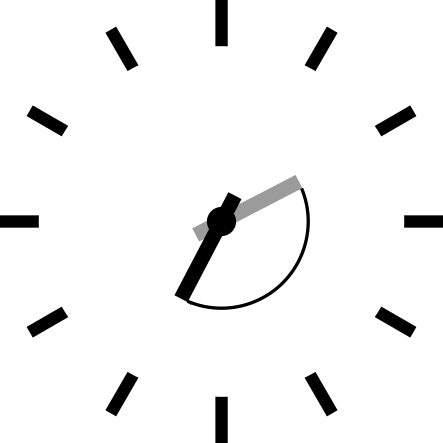
\includegraphics[width=.4\linewidth]{./Illustrations/ModularArithmetic/Clock2Plus5.pdf}
\caption{$2 + 5 = 7$, on the clock.}
\label{fig:Clock2Plus5}
\end{figure}

Similarly, we can subtract times. If it's 10 o'clock now, and you'd
like to know what time it was two hours ago, you subtract two and end
up with 8.

\begin{figure}[ht!]
\centering
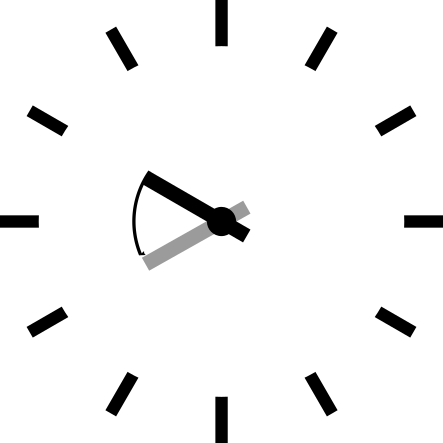
\includegraphics[width=.4\linewidth]{./Illustrations/ModularArithmetic/Clock10Minus2.pdf}
\caption{$10 - 2 = 8$, on the clock.}
\label{fig:ClockMinus}
\end{figure}

The \enquote{weird} part is when you cross the boundary at 12. As far as the
clock is concerned, there's no real difference between 12 and 0. If
it's 10 o'clock now, it'll be 2 o'clock in four hours. If it's 2
o'clock now, it was 9 o'clock five hours ago.

This is an example of what's called \enquote{modular arithmetic}. The
modulus, in this case, is 12. We can write the above equations as:

\[
(10 + 4) \bmod{12} = 2
\]
\[
(2 - 5) \bmod{12} = 9
\]

In these equations, the $\bmod$ is an operator, giving the remainder
after division. When we are dealing with modular arithmetic, where all
operations are affected by the modulus instead of a simple single
operation, we'll write $\negthickspace\pmod{12}$ at the end of the
equation:

\[
10 + 4 \equiv 2 \pmod{12}
\]
\[
2 - 5 \equiv 9 \pmod{12}
\]

This is read as \enquote{ten plus four is equivalent to two, modulo twelve}
and \enquote{two minus five is equivalent to nine, modulo twelve}. That might
seems like a trivial notational hack now, but the difference will
become apparent once we start applying tricks for doing more complex
modular computations, like multiplication and exponentiation.
\section{Prime numbers}
\label{sec-4-1-2}

Prime numbers are wonderful kinds of numbers that come back in many
branches of mathematics. Anything I say about them probably won't do
them justice; but we're in a practical book about applied
cryptography, so we'll only see a few properties.

A prime number is a number that is divisible only by two numbers: 1
and itself. For example, 3 is a prime number, but 4 is not, because it
can be divided by 2.

Any number can be written as a product of prime factors: a bunch of
prime numbers multiplied together. That product is called a
factorization. For example, 30 can be factorized into 2, 3 and 5:

\[
30 = 2 \cdot 3 \cdot 5
\]

Sometimes, a prime number will occur more than once in a
factorization. For example, the factorization of 360 has 2 in it
three times, and three in it twice:

\[
360 = 2^3 \cdot 3^2 \cdot 5
\]

The factorization of any prime number is just that prime number itself.

Two numbers are called coprime when their greatest common divisor is
1, or, to put it in another way, they don't share any prime factors.
Since the only prime factor a prime has is itself, that means that a
prime is coprime to every other number.
\section{Multiplication}
\label{sec-4-1-3}

You might remember you were first taught multiplication as repeated
addition:

\[
n \cdot x = \underbrace{x + x + \ldots + x}_{n \text{ times}}
\]

Modular multiplication is no different. You can compute modular
multiplication by adding the numbers together, and taking the modulus
whenever the sum gets larger than the modulus. You can also just do
regular multiplication, and then take the modulus at the end.
\section{Division and modular inverses}
\label{sec-4-1-4}

Division is defined as the inverse of multiplication. So, $a \cdot b
\equiv c \pmod m$, then $\frac{c}{b} \equiv a \pmod m$.

For example, $5 \cdot 6 \equiv 2 \pmod 7$; so: $\frac{2}{6} \equiv 5
\pmod 7$.

Usually, instead of using division directly, we'll multiply using
something called a modular inverse. The modular inverse of $a$ is a
number, that when you multiply it with $a$, you get 1. This is just
like the inverse of a number in regular arithmetic: $x \cdot
\frac{1}{x} = 1$.

Like in regular arithmetic, not all numbers have modular inverses.
This is the equivalent of dividing by zero in regular arithmetic.

There are two algorithms that are used to compute modular inverses:
the extended Euclidean algorithm, and with the help of Euler's
theorem.

\subsection{The extended Euclidean theorem}
\label{sec-4-1-4-1}

TODO: explain, and how you can get modular inverses with it
\subsection{Using Euler's theorem}
\label{sec-4-1-4-2}

Euler's theorem states that if two numbers $a$ and $n$ are coprime,
then:

\[
a^{\phi(n)} \equiv 1 \pmod n
\]

In that equation, $\phi$ is Euler's totient function, which counts the
amount of numbers that are coprime to its argument.

Multiplying both sides by $a^{-1}$, $a$'s multiplicative inverse, we
get:

\[
a^{\phi(n) - 1} \equiv a^{-1} \pmod n
\]

That gives us a direct formula for computing $a^{-1}$. Unfortunately,
it's still generally less interesting than using the extended
Euclidean algorithm, for two reasons:

\begin{enumerate}
\item It requires computing the totient function, which is generally more
complex than running the extended Euclidean algorithm in the first
place (unless you happen to know $n$'s prime factors)
\item Modular exponentiation is computationally expensive.
\end{enumerate}

One exception to that rule is for prime moduli. Since a prime is
coprime to every other number, and , since there are $p - 1$ numbers
smaller than $p$, $\phi(p) = p - 1$. So, for a prime modulus, the
modular inverse of $a$ is:

\[
a^{\phi(n) - 1} \equiv a^{-1} \pmod n
\]
\section{Exponentiation}
\label{sec-4-1-5}

Like multiplication is taught as as repeated addition, exponentiation
can be thought of as repeated multiplication:

\[
a^n = \underbrace{a \cdot a \cdot \ldots \cdot a}_{n \text{ times}}
\]

\subsection{Performing modular exponentiation}
\label{sec-4-1-5-1}

As with multiplication, it's possible to compute modular
exponentiation by performing regular exponentiation, and then taking
the modulus at the end. However, this is very inefficient,
particularly for large $n$: the product quickly becomes far too large.

Fortunately, it is possible to compute modular exponentiation much
more efficiently. This is done by splitting the problem up into
smaller sub-problems. For example, instead of computing $2^{20}$
directly you could split it up:

\[
2^{20} = (2^{10})^2
\]

$2^{10}$ is something you can compute on your hands: start at 2, which
is $2^1$, and then keep multiplying by two. Every time you multiply by
two, the exponent goes up by 1, so by the time you've counted all your
fingers (assuming you have ten of them), you're done. The result
is 1024. So:

\begin{align*}
2^{20} &\equiv (2^{10} \bmod {15})^2 \pmod {15} \\
       &\equiv (1024 \bmod {15})^2   \pmod {15} \\
       &\equiv 4^2                   \pmod {15} \\
       &\equiv 16                    \pmod {15} \\
       &\equiv 1                     \pmod {15}
\end{align*}

A particularly efficient way to do it on computers, is splitting the
exponent up into a sum of powers of two. This is called binary
exponentiation, or exponentiation by squaring. Suppose we want to
compute $3^{209} \pmod {19}$. First, we split up 209 into a sum of
powers of two. This is process is essentially just writing 209 down in
binary: which would be 0b11010001. That's very practical if the
computation is being performed by a computer, because that's often how
the computer had the number stored in the first place.

\[
  \begin{array}{lllllllll}
  209 &= 1 \cdot 2^{7} &+ 1 \cdot 2^{6} &+ 0 \cdot 2^{5} &+ 1 \cdot 2^{4} &+ 0 \cdot 2^{3} &+ 0 \cdot 2^{2} &+ 0 \cdot 2^{1} &+ 1 \cdot 2^{0} \\
      &= 1 \cdot 128   &+ 1 \cdot 64    &+ 0 \cdot 32    &+ 1 \cdot 16    &+ 0 \cdot 8     &+ 0 \cdot 4     &+ 0 \cdot 2     &+ 1 \cdot 1 \\
      &= 128           &+ 64            &                &+ 16            &                &                &                &+ 1
  \end{array}
\]

We use that expansion into a sum of powers of two to rewrite the equation:

\begin{align*}
3^{209} &= 3^{128 + 64 + 16 + 1} \\
        &= 3^{128} \cdot 3^{64} \cdot 3^{16} \cdot 3^1
\end{align*}

Now, we need to compute those individual powers of 3: 1, 16, 64
and 128. A nice property of this algorithm is that we don't actually
have to compute the big powers separately from scratch. We can use
previously computed smaller powers to compute the larger ones. For
example, we need both $3^{128} \pmod {19}$ and $3^{64} \pmod {19}$, but
you can write the former in terms of the latter:

\[
3^{128} \bmod {19} = (3^{64} \bmod {19})^2 \pmod {19}
\]

Let's compute all the powers of 3 we need. For sake of brevity, we
won't write these out entirely, but remember that all tricks we've
already seen to compute these still apply:

\begin{align*}
3^{16}  &\equiv 17                               \pmod {19} \\
3^{64}  &\equiv (3^{16})^4 \equiv 17^4 \equiv 16 \pmod {19} \\
3^{128} &\equiv (3^{64})^2 \equiv 16^2 \equiv 9  \pmod {19}
\end{align*}

Filling these back in to our old equation:

\begin{align*}
3^{209} &=      3^{128} \cdot 3^{64} \cdot 3^{16} \cdot 3^1 \pmod {19} \\
        &\equiv 9       \cdot 16     \cdot 17     \cdot 3   \pmod {19}
\end{align*}

This trick is particularly interesting when the exponent is a very
large number. That is the case in many cryptographic applications. For
example, in \hyperref[RSA]{RSA} decryption, the exponent is the private key $d$, which
is usually more than a thousand bits long. Keep in mind that this
method will still leak timing information, so it's only suitable for
offline computation. Modular exponentiation can also be computed using
a technique called a Montgomery ladder, which we'll see in the next
section.

Many programming languages provide access to specific modular
exponentiation functions. For example, in Python, \verb~pow(e, x, m)~
performs efficient modular exponentiation. However, the expression
\verb~(e ** x) % m~ will still use the inefficient method.
\subsection{Timing-invariant computation using a Montgomery ladder}
\label{sec-4-1-5-2}

TODO: explain
\section{Discrete logarithm}
\label{sec-4-1-6}

Just like subtraction is the inverse of addition, and division is the
inverse of multiplication, logarithms are the inverse of
exponentiation. In regular arithmetic, $e^x = y$, if $x = \log_e y$.
The equivalent of this in modular arithmetic is commonly called a
\enquote{discrete logarithm}.

As with division, if you start from the definition as the inverse of a
different operator, it's easy to come up with examples. For example,
since $3^6 \equiv 9 \pmod {15}$, we can define $9 \equiv \log_3 6
\pmod {15}$. However computing discrete logarithms is generally fairly
hard, unlike modular inverses. There is no formal proof that computing
discrete logarithms is complex; we just haven't found any efficient
algorithms to do it.

There is one theoretical algorithm for computing discrete logarithms
efficiently. However, it requires a quantum computer, which is a
fundamentally different kind of computer from the classical computers
we use today. While we can build such computers, we can only build
very small ones. The limited size of our quantum computers strongly
limits which problems we can solve. So far, they're much more in the
realm of the kind of arithmetic a child can do in their head, than
ousting the top of the line classical computers from the performance
throne.

The complexity of computing discrete logarithms, together with the
relative simplicity of computing its inverse, modular exponentiation,
is the basis for many public key cryptosystems. Common examples
include the \hyperref[RSA]{RSA} encryption primitive, or the Diffie-Hellman key
exchange protocol.

While cryptosystems based on the discrete logarithm problem are
currently considered secure with appropriate parameter choices, there
are certainly ways that could change in the future. For example:

\begin{itemize}
\item Theoretical breakthroughs in number theory could make discrete logarithms
significantly easier to compute than we currently think.
\item Technological breakthroughs in quantum computing could lead to large
enough quantum computers.
\item Technological breakthroughs in classical computing as well as the
continuous gradual increases in performance and decreases in cost
could increase the size of some problems that can be tackled using
classical computers.
\end{itemize}

Discrete logarithm computation is tightly linked to the problem of
number factorization. They are still areas of active mathematical
research; the links between the two problems are not still not
thoroughly understood. That said, there are many similarities between
the two:

\begin{itemize}
\item Both are believed to be hard to compute on classical computers, but
neither has a proof of that fact.
\item They can both be efficiently computed on quantum computers using
Shor's algorithm.
\item Mathematical advances in one are typically quickly turned into
mathematical advances in the other.
\end{itemize}
\chapter{Elliptic curves\label{Elliptic-curves}}
\label{sec-4-2}

Like modular arithmetic, elliptic curve arithmetic is used for many
public key cryptosystems. Many cryptosystems that traditionally work
with modular arithmetic, such as Diffie-Hellman and DSA, have an
elliptic curve counterpart.

Elliptic curves are curves with the following form:

\[
y^2 = x^3 - ax + b
\]

This is the most common form when talking about elliptic curves in
general; there are several other forms which mostly have applications
in cryptography, notably the Edwards form:

\[
x^2 + y^2 = 1 + dx^2y^2
\]

We can define addition of points on the curve.

TODO: Move the Abelian group thing somewhere else, since it applies to
our fields thing as well

All of this put together form something called an Abelian group.
That's a scary-sounding mathematical term that almost everyone already
understands the basics of. Specifically, if you know how to add
integers ($\ldots -2, -1, 0, 1, 2, \ldots$) together, you already know
an Abelian group. An Abelian group satisfies five properties:

\begin{enumerate}
\item If $a$ and $b$ are members of the Abelian group and $\star$ is the
operator, then $a \star b$ is also a member of that Abelian group.
Indeed, any two integers added together always get you another
integer. This property is called \emph{closure}, or, we say that the
group is \emph{closed under addition} (or whatever the name is of the
operation we've defined).
\item If $a$, $b$ and $c$ are members of the Abelian group, the order of
operations doesn't matter; to put it differently: we can move the
brackets around. In equation form: $(a \star b) \star c = a \star
   (b \star c)$. Indeed, the order in which you add integers together
doesn't matter; they will always sum up to the same value. This
property is called \emph{associativity}, and the group is said to be
\emph{associative}.
\item There's exactly one identity element $i$, for which $a \star i = i
   \star a = a$. For integer addition, that's zero: $a + 0 = 0 + a =
   a$ for all a.
\item For each element $a$, there's exactly one inverse element $b$, for
which $a \star b = b \star a = i$, where $i$ is the identity
element. Indeed, for integer addition, $a + (-a) = (-a) + a = 0$
for all a.
\item The order of elements doesn't matter for the result of the
operation. For all elements $a, b$, $a \star b = b \star a$. This
is known as \emph{commutativity}, and the group is said to be
\emph{commutative}.
\end{enumerate}

The first four properties are called group properties and make
something a group; the last property is what makes a group Abelian.

We can see that our elliptic curve, with the point at infinity and the
addition operator, forms an Abelian group:

\begin{enumerate}
\item If $P$ and $Q$ are two points on the elliptic curve, then $P + Q$
   is also always a point on the curve.
\item If $P$, $Q$, and $R$ are all points on the curve, then $P + (Q + R)
   = (P + Q) + R$, so the elliptic curve is associative.
\item There's an identity element, our point at infinity $O$. For all
points on the curve $P$, $P + O = O + P = P$.
\item Each element has an inverse element. This is easiest explained
visually TODO: Explain visually
\item The order of operations doesn't matter, $P + Q = Q + P$ for all $P,
   Q$ on the curve.
\end{enumerate}

\section{The elliptic curve discrete log problem}
\label{sec-4-2-1}

TOOD: explain fully

As with the regular discrete log problem, the elliptic curve discrete
log problem doesn't actually have a formal proof that the operation is
\enquote{hard} to perform: we just know that there is no publicly available
algorithm to do it efficiently. It's possible, however unlikely, that
someone has a magical algorithm that makes the problem easy, and that
would break elliptic curve cryptography completely. It's far more
likely that we will see a stream of continuous improvements, which
coupled with increased computing power eventually eat away at the
security of the algorithm.
\chapter{Side-channel attacks}
\label{sec-4-3}
\section{Timing attacks}
\label{sec-4-3-1}
\subsection{AES cache timing}
\label{sec-4-3-1-1}

\url{http://tau.ac.il/~tromer/papers/cache.pdf}
\subsection{Elliptic curve timing attacks}
\label{sec-4-3-1-2}

TODO: Explain why the edwards form is great?
\section{Power measurement attacks}
\label{sec-4-3-2}
TODO: Say something here.

\bibliographystyle{plain}
\bibliography{Crypto101}

\setglossarystyle{altlisthypergroup}
\glsaddall
\printglossaries
% Emacs 24.3.1 (Org mode 8.2.5h)
\end{document}
